\documentclass[11pt,a4paper]{article}
\usepackage[margin=2cm]{geometry}
\usepackage{lmodern}
\usepackage[T1]{fontenc}
\usepackage{amsmath,amssymb}
\usepackage{booktabs,array,tabularx,xltabular}
\usepackage{enumitem}
\usepackage{xcolor}
\usepackage[most]{tcolorbox}
\usepackage{titlesec}
\usepackage{graphicx}
\usepackage{float}
\usepackage[font=small,labelfont={bf,color=headblue},skip=4pt]{caption}
\usepackage[colorlinks=true,linkcolor=headblue,urlcolor=blue!50!black]{hyperref}

\definecolor{headblue}{RGB}{38,70,120}
\titleformat{\section}{\Large\bfseries\color{headblue}}{\thesection}{0.8em}{}[{\color{black}\titlerule}]
\titleformat{\subsection}{\large\bfseries\color{headblue}}{\thesubsection}{0.8em}{}
\titleformat{\subsubsection}{\normalsize\bfseries\color{headblue}}{\thesubsubsection}{0.8em}{}
\titlespacing*{\section}{0pt}{12pt}{6pt}
\titlespacing*{\subsection}{0pt}{9pt}{3pt}
\titlespacing*{\subsubsection}{0pt}{7pt}{2pt}
\setlength{\parindent}{0pt}
\setlength{\parskip}{5pt}
\setlist{itemsep=2pt,topsep=2pt}
\setlength{\emergencystretch}{3em}
\renewcommand{\arraystretch}{1.12}
\setlength{\tabcolsep}{4.5pt}
\setlength{\LTpre}{2pt}\setlength{\LTpost}{2pt}
\allowdisplaybreaks
\newtcolorbox{keybox}{colback=blue!3,colframe=headblue!60,boxrule=0.5pt,arc=2mm,left=2mm,right=2mm,top=1mm,bottom=1mm}
\newtcolorbox{insum}{colback=green!3,colframe=green!40!black,boxrule=0.4pt,arc=1.5mm,left=2mm,right=2mm,top=0.5mm,bottom=0.5mm,fontupper=\small}
\newcommand{\inshort}[1]{\begin{insum}\textbf{In short.} #1\end{insum}}
\newcommand{\pct}{\,\%}
\newcommand{\code}[1]{\texttt{#1}}
% title block shared by the three reports: \reporttitle{subtitle}
\newcommand{\reporttitle}[1]{%
\begin{center}
{\LARGE\bfseries\color{headblue} EV Charging with Personal and Commercial Customers\\[2pt] (Formulation 4)}\\[8pt]
{\large #1}\\[6pt]
{\normalsize CP 320 Operations Research for Mobility, course project}\\[2pt]
{\normalsize Yakshith Maddineni (SR 26080) \quad\textperiodcentered\quad Kartikeya Gaur (SR 26371)}\\[2pt]
{\normalsize 27 November 2026}
\end{center}}

\usepackage{adjustbox}
\newcommand{\AgreeAll}{94.8}
\newcommand{\AgreeCommercial}{98.9}
\newcommand{\AgreeFree}{93.8}
\newcommand{\AgreePersonal}{82.0}
\newcommand{\AgreeStation}{78.9}
\newcommand{\AgreeStrandedVan}{100}
\newcommand{\BandKeysEight}{473}
\newcommand{\BandKeysFive}{470}
\newcommand{\BandKeysNine}{393}
\newcommand{\BandKeysOne}{470}
\newcommand{\BandKeysSix}{472}
\newcommand{\BandKeysTen}{421}
\newcommand{\BandKeysTwo}{441}
\newcommand{\BaseBestVal}{0.969}
\newcommand{\BothValid}{474}
\newcommand{\CcComEeightBatHiMilp}{+0.1}
\newcommand{\CcComEeightBatHiRt}{$-$0.5}
\newcommand{\CcComEeightBatHiZs}{+0.1}
\newcommand{\CcComEfiveComHiMilp}{+5.5}
\newcommand{\CcComEfiveComHiRt}{+5.2}
\newcommand{\CcComEfiveComHiZs}{+5.8}
\newcommand{\CcComEfiveComLoMilp}{$-$5.6}
\newcommand{\CcComEfiveComLoRt}{$-$6.3}
\newcommand{\CcComEfiveComLoZs}{$-$5.8}
\newcommand{\CcComEfivePersHiMilp}{$-$0.1}
\newcommand{\CcComEfivePersHiRt}{$-$0.7}
\newcommand{\CcComEfivePersHiZs}{$-$0.0}
\newcommand{\CcComEfivePersLoMilp}{+0.1}
\newcommand{\CcComEfivePersLoRt}{$-$0.3}
\newcommand{\CcComEfivePersLoZs}{+0.1}
\newcommand{\CcComEnineGunsHiRt}{$-$3.7}
\newcommand{\CcComEnineGunsLoRt}{+5.1}
\newcommand{\CcComEninePowHiRt}{$-$14.2}
\newcommand{\CcComEninePowLoRt}{+24.6}
\newcommand{\CcComEonePMHiMilp}{+6.0}
\newcommand{\CcComEonePMHiRt}{+5.7}
\newcommand{\CcComEonePMHiZs}{+5.8}
\newcommand{\CcComEonePMLoMilp}{$-$6.1}
\newcommand{\CcComEonePMLoRt}{$-$6.2}
\newcommand{\CcComEonePMLoZs}{$-$5.7}
\newcommand{\CcComEsixComHiMilp}{+14.0}
\newcommand{\CcComEsixComHiRt}{+13.2}
\newcommand{\CcComEsixComHiZs}{+13.8}
\newcommand{\CcComEsixComLoMilp}{$-$14.0}
\newcommand{\CcComEsixComLoRt}{$-$14.0}
\newcommand{\CcComEsixComLoZs}{$-$13.8}
\newcommand{\CcComEsixPersHiMilp}{$-$0.0}
\newcommand{\CcComEsixPersHiRt}{$-$0.3}
\newcommand{\CcComEsixPersHiZs}{$-$0.1}
\newcommand{\CcComEsixPersLoMilp}{$-$0.1}
\newcommand{\CcComEsixPersLoRt}{$-$0.4}
\newcommand{\CcComEsixPersLoZs}{+0.0}
\newcommand{\CcComEtenDemHiRt}{+23.2}
\newcommand{\CcComEtenDemLoRt}{$-$24.1}
\newcommand{\CcComEtwoSeatsHiMilp}{+0.1}
\newcommand{\CcComEtwoSeatsHiRt}{+0.1}
\newcommand{\CcComEtwoSeatsHiZs}{+0.2}
\newcommand{\CcComEtwoSeatsLoMilp}{$-$0.3}
\newcommand{\CcComEtwoSeatsLoRt}{$-$0.8}
\newcommand{\CcComEtwoSeatsLoZs}{$-$0.4}
\newcommand{\CcComEtwoVansHiMilp}{$-$0.0}
\newcommand{\CcComEtwoVansHiRt}{$-$0.3}
\newcommand{\CcComEtwoVansHiZs}{+0.0}
\newcommand{\CcComEtwoVansLoMilp}{+0.1}
\newcommand{\CcComEtwoVansLoRt}{$-$0.0}
\newcommand{\CcComEtwoVansLoZs}{+0.1}
\newcommand{\CcComLowEonePMHi}{+4.5}
\newcommand{\CcComLowEonePMLo}{$-$5.0}
\newcommand{\CcPersEeightBatHiMilp}{+0.5}
\newcommand{\CcPersEeightBatHiRt}{+0.7}
\newcommand{\CcPersEeightBatHiZs}{$-$0.0}
\newcommand{\CcPersEfiveComHiMilp}{+0.3}
\newcommand{\CcPersEfiveComHiRt}{+1.3}
\newcommand{\CcPersEfiveComHiZs}{+0.0}
\newcommand{\CcPersEfiveComLoMilp}{$-$0.2}
\newcommand{\CcPersEfiveComLoRt}{+1.2}
\newcommand{\CcPersEfiveComLoZs}{$-$0.1}
\newcommand{\CcPersEfivePersHiMilp}{+5.7}
\newcommand{\CcPersEfivePersHiRt}{+10.1}
\newcommand{\CcPersEfivePersHiZs}{+10.0}
\newcommand{\CcPersEfivePersLoMilp}{$-$8.1}
\newcommand{\CcPersEfivePersLoRt}{$-$8.9}
\newcommand{\CcPersEfivePersLoZs}{$-$10.4}
\newcommand{\CcPersEnineGunsHiRt}{$-$1.5}
\newcommand{\CcPersEnineGunsLoRt}{+3.4}
\newcommand{\CcPersEninePowHiRt}{$-$22.9}
\newcommand{\CcPersEninePowLoRt}{+7.3}
\newcommand{\CcPersEonePMHiMilp}{+7.2}
\newcommand{\CcPersEonePMHiRt}{+5.6}
\newcommand{\CcPersEonePMHiZs}{+4.6}
\newcommand{\CcPersEonePMLoMilp}{$-$11.1}
\newcommand{\CcPersEonePMLoRt}{$-$5.2}
\newcommand{\CcPersEonePMLoZs}{$-$5.1}
\newcommand{\CcPersEsixComHiMilp}{+0.1}
\newcommand{\CcPersEsixComHiRt}{+0.9}
\newcommand{\CcPersEsixComHiZs}{+0.0}
\newcommand{\CcPersEsixComLoMilp}{+0.1}
\newcommand{\CcPersEsixComLoRt}{+0.8}
\newcommand{\CcPersEsixComLoZs}{$-$0.0}
\newcommand{\CcPersEsixPersHiMilp}{+6.3}
\newcommand{\CcPersEsixPersHiRt}{+6.3}
\newcommand{\CcPersEsixPersHiZs}{+5.9}
\newcommand{\CcPersEsixPersLoMilp}{$-$5.9}
\newcommand{\CcPersEsixPersLoRt}{$-$4.8}
\newcommand{\CcPersEsixPersLoZs}{$-$5.8}
\newcommand{\CcPersEtenDemHiRt}{+24.1}
\newcommand{\CcPersEtenDemLoRt}{$-$21.9}
\newcommand{\CcPersEtwoSeatsHiMilp}{$-$0.1}
\newcommand{\CcPersEtwoSeatsHiRt}{+0.4}
\newcommand{\CcPersEtwoSeatsHiZs}{+0.1}
\newcommand{\CcPersEtwoSeatsLoMilp}{+1.4}
\newcommand{\CcPersEtwoSeatsLoRt}{+0.3}
\newcommand{\CcPersEtwoSeatsLoZs}{$-$0.3}
\newcommand{\CcPersEtwoVansHiMilp}{$-$0.1}
\newcommand{\CcPersEtwoVansHiRt}{+0.6}
\newcommand{\CcPersEtwoVansHiZs}{$-$0.0}
\newcommand{\CcPersEtwoVansLoMilp}{+0.5}
\newcommand{\CcPersEtwoVansLoRt}{+0.5}
\newcommand{\CcPersEtwoVansLoZs}{+0.2}
\newcommand{\CcPersTopEonePMHi}{+10.1}
\newcommand{\CcPersTopEonePMLo}{$-$15.4}
\newcommand{\ComFcsUsersTheta}{0.36}
\newcommand{\ComHighNOpt}{72}
\newcommand{\ComHighQueueOpt}{0.00}
\newcommand{\ComHighQueueTL}{7.22}
\newcommand{\ComVanInOptimal}{0}
\newcommand{\ComVanInOptimalAll}{0}
\newcommand{\ComVanInTL}{103}
\newcommand{\ComVanOffPeak}{103}
\newcommand{\ComVanUsers}{103}
\newcommand{\ComVanUsersHighShare}{98}
\newcommand{\ComVanUsersTheta}{0.24}
\newcommand{\CorrEeightBatHi}{0.08}
\newcommand{\CorrEfiveComHi}{0.49}
\newcommand{\CorrEfiveComLo}{0.56}
\newcommand{\CorrEfivePersHi}{0.75}
\newcommand{\CorrEfivePersLo}{0.76}
\newcommand{\CorrEonePMHi}{0.79}
\newcommand{\CorrEonePMLo}{0.81}
\newcommand{\CorrEsixComHi}{0.82}
\newcommand{\CorrEsixComLo}{0.79}
\newcommand{\CorrEsixPersHi}{0.44}
\newcommand{\CorrEsixPersLo}{0.43}
\newcommand{\CorrEtwoSeatsHi}{0.23}
\newcommand{\CorrEtwoSeatsLo}{0.74}
\newcommand{\CorrEtwoVansHi}{$-$0.17}
\newcommand{\CorrEtwoVansLo}{0.00}
\newcommand{\DZsixRl}{+2.00}
\newcommand{\DZthreeRl}{$-$0.40}
\newcommand{\DirBad}{0}
\newcommand{\DirMeanEeightBatHi}{$-$0.04}
\newcommand{\DirMeanEfiveComHi}{+2.50}
\newcommand{\DirMeanEfiveComLo}{$-$2.51}
\newcommand{\DirMeanEfivePersHi}{+1.95}
\newcommand{\DirMeanEfivePersLo}{$-$2.19}
\newcommand{\DirMeanEonePMHi}{+4.07}
\newcommand{\DirMeanEonePMLo}{$-$4.45}
\newcommand{\DirMeanEsixComHi}{+6.46}
\newcommand{\DirMeanEsixComLo}{$-$6.45}
\newcommand{\DirMeanEsixPersHi}{+1.30}
\newcommand{\DirMeanEsixPersLo}{$-$1.30}
\newcommand{\DirMeanEtwoSeatsHi}{$-$0.16}
\newcommand{\DirMeanEtwoSeatsLo}{+1.30}
\newcommand{\DirMeanEtwoVansHi}{$-$0.00}
\newcommand{\DirMeanEtwoVansLo}{+0.00}
\newcommand{\DirNEeightBatHi}{274}
\newcommand{\DirNEfiveComHi}{275}
\newcommand{\DirNEfiveComLo}{275}
\newcommand{\DirNEfivePersHi}{252}
\newcommand{\DirNEfivePersLo}{275}
\newcommand{\DirNEonePMHi}{276}
\newcommand{\DirNEonePMLo}{225}
\newcommand{\DirNEsixComHi}{275}
\newcommand{\DirNEsixComLo}{272}
\newcommand{\DirNEsixPersHi}{276}
\newcommand{\DirNEsixPersLo}{273}
\newcommand{\DirNEtwoSeatsHi}{263}
\newcommand{\DirNEtwoSeatsLo}{275}
\newcommand{\DirNEtwoVansHi}{273}
\newcommand{\DirNEtwoVansLo}{275}
\newcommand{\DirPairs}{4,034}
\newcommand{\DownBEnineGunsHiRt}{67.0}
\newcommand{\DownBEnineGunsLoRt}{63.7}
\newcommand{\DownBEninePowHiRt}{67.0}
\newcommand{\DownBEninePowLoRt}{63.3}
\newcommand{\DownBEtenDemHiRt}{64.2}
\newcommand{\DownBEtenDemLoRt}{67.0}
\newcommand{\DownEnineGunsHiRt}{61.7}
\newcommand{\DownEnineGunsLoRt}{70.6}
\newcommand{\DownEninePowHiRt}{40.8}
\newcommand{\DownEninePowLoRt}{107.5}
\newcommand{\DownEtenDemHiRt}{77.5}
\newcommand{\DownEtenDemLoRt}{52.0}
\newcommand{\EeightAbs}{0.01}
\newcommand{\EeightDecision}{below}
\newcommand{\EeightOptChanged}{34}
\newcommand{\EffDiffRtMax}{0.41}
\newcommand{\EffDiffRtMean}{0.16}
\newcommand{\EffDiffZsMax}{0.45}
\newcommand{\EffDiffZsMean}{0.14}
\newcommand{\ElastEnergyRl}{+0.880}
\newcommand{\ElastGunsRl}{$-$0.047}
\newcommand{\ElastPowerRl}{$-$0.216}
\newcommand{\GapMax}{4.8}
\newcommand{\GapMean}{0.85}
\newcommand{\GapMedian}{0.76}
\newcommand{\GapOpt}{0.92}
\newcommand{\GapPninety}{2.00}
\newcommand{\GapRtAll}{0.87}
\newcommand{\GapRtEeightBatHi}{0.77}
\newcommand{\GapRtEfiveComHi}{0.86}
\newcommand{\GapRtEfiveComLo}{0.98}
\newcommand{\GapRtEfivePersHi}{1.14}
\newcommand{\GapRtEfivePersLo}{0.56}
\newcommand{\GapRtEonePMHi}{0.63}
\newcommand{\GapRtEonePMLo}{1.25}
\newcommand{\GapRtEsixComHi}{0.79}
\newcommand{\GapRtEsixComLo}{0.91}
\newcommand{\GapRtEsixPersHi}{0.84}
\newcommand{\GapRtEsixPersLo}{0.95}
\newcommand{\GapRtEtwoSeatsHi}{0.98}
\newcommand{\GapRtEtwoSeatsLo}{0.65}
\newcommand{\GapRtEtwoVansHi}{0.81}
\newcommand{\GapRtEtwoVansLo}{0.96}
\newcommand{\GapTL}{0.76}
\newcommand{\GapVarMax}{1.31}
\newcommand{\GapVarMin}{0.56}
\newcommand{\GapZsAll}{0.86}
\newcommand{\GapZsEeightBatHi}{0.84}
\newcommand{\GapZsEfiveComHi}{0.83}
\newcommand{\GapZsEfiveComLo}{0.82}
\newcommand{\GapZsEfivePersHi}{1.22}
\newcommand{\GapZsEfivePersLo}{0.56}
\newcommand{\GapZsEonePMHi}{0.58}
\newcommand{\GapZsEonePMLo}{1.31}
\newcommand{\GapZsEsixComHi}{0.80}
\newcommand{\GapZsEsixComLo}{0.87}
\newcommand{\GapZsEsixPersHi}{0.80}
\newcommand{\GapZsEsixPersLo}{0.92}
\newcommand{\GapZsEtwoSeatsHi}{0.86}
\newcommand{\GapZsEtwoSeatsLo}{0.69}
\newcommand{\GapZsEtwoVansHi}{0.84}
\newcommand{\GapZsEtwoVansLo}{0.91}
\newcommand{\JobEnd}{2026-11-25 06:04}
\newcommand{\JobHours}{56}
\newcommand{\JobLogRev}{9ce6b13}
\newcommand{\JobNonZero}{0}
\newcommand{\JobStart}{2026-11-22 21:45}
\newcommand{\LostEeightBatHiMilp}{1}
\newcommand{\LostEeightBatHiRt}{1}
\newcommand{\LostEeightBatHiZs}{0}
\newcommand{\LostEfiveComHiMilp}{2}
\newcommand{\LostEfiveComHiRt}{1}
\newcommand{\LostEfiveComHiZs}{0}
\newcommand{\LostEfiveComLoMilp}{3}
\newcommand{\LostEfiveComLoRt}{1}
\newcommand{\LostEfiveComLoZs}{1}
\newcommand{\LostEfivePersHiMilp}{2}
\newcommand{\LostEfivePersHiRt}{0}
\newcommand{\LostEfivePersHiZs}{0}
\newcommand{\LostEfivePersLoMilp}{2}
\newcommand{\LostEfivePersLoRt}{1}
\newcommand{\LostEfivePersLoZs}{1}
\newcommand{\LostEnineGunsHiRt}{0}
\newcommand{\LostEnineGunsLoRt}{68}
\newcommand{\LostEninePowHiRt}{0}
\newcommand{\LostEninePowLoRt}{102}
\newcommand{\LostEonePMHiMilp}{0}
\newcommand{\LostEonePMHiRt}{1}
\newcommand{\LostEonePMHiZs}{2}
\newcommand{\LostEonePMLoMilp}{4}
\newcommand{\LostEonePMLoRt}{1}
\newcommand{\LostEonePMLoZs}{1}
\newcommand{\LostEsixComHiMilp}{1}
\newcommand{\LostEsixComHiRt}{1}
\newcommand{\LostEsixComHiZs}{1}
\newcommand{\LostEsixComLoMilp}{0}
\newcommand{\LostEsixComLoRt}{0}
\newcommand{\LostEsixComLoZs}{1}
\newcommand{\LostEsixPersHiMilp}{1}
\newcommand{\LostEsixPersHiRt}{1}
\newcommand{\LostEsixPersHiZs}{1}
\newcommand{\LostEsixPersLoMilp}{2}
\newcommand{\LostEsixPersLoRt}{0}
\newcommand{\LostEsixPersLoZs}{1}
\newcommand{\LostEtenDemHiRt}{79}
\newcommand{\LostEtenDemLoRt}{0}
\newcommand{\LostEtwoSeatsHiMilp}{3}
\newcommand{\LostEtwoSeatsHiRt}{1}
\newcommand{\LostEtwoSeatsHiZs}{1}
\newcommand{\LostEtwoSeatsLoMilp}{7}
\newcommand{\LostEtwoSeatsLoRt}{6}
\newcommand{\LostEtwoSeatsLoZs}{7}
\newcommand{\LostEtwoVansHiMilp}{0}
\newcommand{\LostEtwoVansHiRt}{0}
\newcommand{\LostEtwoVansHiZs}{0}
\newcommand{\LostEtwoVansLoMilp}{33}
\newcommand{\LostEtwoVansLoRt}{34}
\newcommand{\LostEtwoVansLoZs}{35}
\newcommand{\LostFamEnineGunsHiCone}{0}
\newcommand{\LostFamEnineGunsHiCtwo}{0}
\newcommand{\LostFamEnineGunsHiRCone}{0}
\newcommand{\LostFamEnineGunsHiRCtwo}{0}
\newcommand{\LostFamEnineGunsHiRone}{0}
\newcommand{\LostFamEnineGunsHiRtwo}{0}
\newcommand{\LostFamEnineGunsLoCone}{4}
\newcommand{\LostFamEnineGunsLoCtwo}{4}
\newcommand{\LostFamEnineGunsLoRCone}{22}
\newcommand{\LostFamEnineGunsLoRCtwo}{3}
\newcommand{\LostFamEnineGunsLoRone}{28}
\newcommand{\LostFamEnineGunsLoRtwo}{7}
\newcommand{\LostFamEninePowHiCone}{0}
\newcommand{\LostFamEninePowHiCtwo}{0}
\newcommand{\LostFamEninePowHiRCone}{0}
\newcommand{\LostFamEninePowHiRCtwo}{0}
\newcommand{\LostFamEninePowHiRone}{0}
\newcommand{\LostFamEninePowHiRtwo}{0}
\newcommand{\LostFamEninePowLoCone}{3}
\newcommand{\LostFamEninePowLoCtwo}{3}
\newcommand{\LostFamEninePowLoRCone}{44}
\newcommand{\LostFamEninePowLoRCtwo}{3}
\newcommand{\LostFamEninePowLoRone}{45}
\newcommand{\LostFamEninePowLoRtwo}{4}
\newcommand{\LostFamEtenDemHiCone}{2}
\newcommand{\LostFamEtenDemHiCtwo}{1}
\newcommand{\LostFamEtenDemHiRCone}{39}
\newcommand{\LostFamEtenDemHiRCtwo}{1}
\newcommand{\LostFamEtenDemHiRone}{34}
\newcommand{\LostFamEtenDemHiRtwo}{2}
\newcommand{\LostFamEtenDemLoCone}{0}
\newcommand{\LostFamEtenDemLoCtwo}{0}
\newcommand{\LostFamEtenDemLoRCone}{0}
\newcommand{\LostFamEtenDemLoRCtwo}{0}
\newcommand{\LostFamEtenDemLoRone}{0}
\newcommand{\LostFamEtenDemLoRtwo}{0}
\newcommand{\LostGunsLoMinN}{50}
\newcommand{\MfcsRvanCommercial}{74}
\newcommand{\MfcsRvanPersonal}{138}
\newcommand{\MilpCPUh}{87}
\newcommand{\MilpInfeasible}{51}
\newcommand{\MilpOnly}{0}
\newcommand{\MilpOptimal}{277}
\newcommand{\MilpSolveMean}{140}
\newcommand{\MilpTL}{197}
\newcommand{\MilpTLnoPlan}{35}
\newcommand{\MilpValid}{474}
\newcommand{\MvanRfcsCommercial}{78}
\newcommand{\MvanRfcsPersonal}{959}
\newcommand{\NFactorsAll}{11}
\newcommand{\NInst}{560}
\newcommand{\NRuns}{47}
\newcommand{\NVariants}{15}
\newcommand{\NVariantsRl}{6}
\newcommand{\NeitherValid}{60}
\newcommand{\NewEeightBatHiMilp}{3}
\newcommand{\NewEeightBatHiRt}{1}
\newcommand{\NewEeightBatHiZs}{1}
\newcommand{\NewEfiveComHiMilp}{3}
\newcommand{\NewEfiveComHiRt}{0}
\newcommand{\NewEfiveComHiZs}{0}
\newcommand{\NewEfiveComLoMilp}{1}
\newcommand{\NewEfiveComLoRt}{1}
\newcommand{\NewEfiveComLoZs}{1}
\newcommand{\NewEfivePersHiMilp}{1}
\newcommand{\NewEfivePersHiRt}{0}
\newcommand{\NewEfivePersHiZs}{2}
\newcommand{\NewEfivePersLoMilp}{1}
\newcommand{\NewEfivePersLoRt}{1}
\newcommand{\NewEfivePersLoZs}{0}
\newcommand{\NewEnineGunsHiRt}{9}
\newcommand{\NewEnineGunsLoRt}{0}
\newcommand{\NewEninePowHiRt}{32}
\newcommand{\NewEninePowLoRt}{0}
\newcommand{\NewEonePMHiMilp}{3}
\newcommand{\NewEonePMHiRt}{1}
\newcommand{\NewEonePMHiZs}{1}
\newcommand{\NewEonePMLoMilp}{1}
\newcommand{\NewEonePMLoRt}{0}
\newcommand{\NewEonePMLoZs}{1}
\newcommand{\NewEsixComHiMilp}{2}
\newcommand{\NewEsixComHiRt}{1}
\newcommand{\NewEsixComHiZs}{1}
\newcommand{\NewEsixComLoMilp}{1}
\newcommand{\NewEsixComLoRt}{0}
\newcommand{\NewEsixComLoZs}{0}
\newcommand{\NewEsixPersHiMilp}{2}
\newcommand{\NewEsixPersHiRt}{0}
\newcommand{\NewEsixPersHiZs}{1}
\newcommand{\NewEsixPersLoMilp}{1}
\newcommand{\NewEsixPersLoRt}{1}
\newcommand{\NewEsixPersLoZs}{1}
\newcommand{\NewEtenDemHiRt}{0}
\newcommand{\NewEtenDemLoRt}{39}
\newcommand{\NewEtwoSeatsHiMilp}{0}
\newcommand{\NewEtwoSeatsHiRt}{0}
\newcommand{\NewEtwoSeatsHiZs}{1}
\newcommand{\NewEtwoSeatsLoMilp}{4}
\newcommand{\NewEtwoSeatsLoRt}{0}
\newcommand{\NewEtwoSeatsLoZs}{0}
\newcommand{\NewEtwoVansHiMilp}{13}
\newcommand{\NewEtwoVansHiRt}{6}
\newcommand{\NewEtwoVansHiZs}{6}
\newcommand{\NewEtwoVansLoMilp}{0}
\newcommand{\NewEtwoVansLoRt}{0}
\newcommand{\NewEtwoVansLoZs}{0}
\newcommand{\OffHighShare}{15}
\newcommand{\POffVanCommercialMilp}{1.1}
\newcommand{\POffVanCommercialRl}{1.0}
\newcommand{\POffVanPersonalMilp}{20.6}
\newcommand{\POffVanPersonalRl}{7.1}
\newcommand{\PPeakVanCommercialMilp}{0.0}
\newcommand{\PPeakVanCommercialRl}{0.0}
\newcommand{\PPeakVanPersonalMilp}{18.4}
\newcommand{\PPeakVanPersonalRl}{4.9}
\newcommand{\PQueueComHighPoorMilp}{10.9}
\newcommand{\PQueueCommercialHighMilp}{7.04}
\newcommand{\PQueueCommercialHighRl}{10.49}
\newcommand{\PQueueCommercialLowMilp}{0.04}
\newcommand{\PQueueCommercialLowRl}{0.16}
\newcommand{\PQueueCommercialMidMilp}{0.33}
\newcommand{\PQueueCommercialMidRl}{0.89}
\newcommand{\PQueuePersHighRichMilp}{0.16}
\newcommand{\PQueuePersonalHighMilp}{1.67}
\newcommand{\PQueuePersonalHighRl}{1.45}
\newcommand{\PQueuePersonalLowMilp}{0.00}
\newcommand{\PQueuePersonalLowRl}{0.02}
\newcommand{\PQueuePersonalMidMilp}{0.06}
\newcommand{\PQueuePersonalMidRl}{0.12}
\newcommand{\PVanCommercialHighMilp}{3.4}
\newcommand{\PVanCommercialHighRl}{3.3}
\newcommand{\PVanCommercialLowMilp}{0.0}
\newcommand{\PVanCommercialLowRl}{0.0}
\newcommand{\PVanCommercialMidMilp}{0.0}
\newcommand{\PVanCommercialMidRl}{0.0}
\newcommand{\PVanPersonalHighMilp}{16.6}
\newcommand{\PVanPersonalHighRl}{2.6}
\newcommand{\PVanPersonalLowMilp}{23.4}
\newcommand{\PVanPersonalLowRl}{9.4}
\newcommand{\PVanPersonalMidMilp}{17.1}
\newcommand{\PVanPersonalMidRl}{4.8}
\newcommand{\PXEeightBatHiQBCommercialHigh}{7.02}
\newcommand{\PXEeightBatHiQBCommercialLow}{0.04}
\newcommand{\PXEeightBatHiQBCommercialMid}{0.33}
\newcommand{\PXEeightBatHiQBPersonalHigh}{1.65}
\newcommand{\PXEeightBatHiQBPersonalLow}{0.00}
\newcommand{\PXEeightBatHiQBPersonalMid}{0.05}
\newcommand{\PXEeightBatHiQCommercialHigh}{$-$0.10}
\newcommand{\PXEeightBatHiQCommercialLow}{+0.00}
\newcommand{\PXEeightBatHiQCommercialMid}{$-$0.01}
\newcommand{\PXEeightBatHiQPersonalHigh}{+0.44}
\newcommand{\PXEeightBatHiQPersonalLow}{+0.00}
\newcommand{\PXEeightBatHiQPersonalMid}{+0.02}
\newcommand{\PXEeightBatHiRtVanComHigh}{$-$1.03}
\newcommand{\PXEeightBatHiRtVanComLow}{$-$0.03}
\newcommand{\PXEeightBatHiRtVanComMid}{+0.04}
\newcommand{\PXEeightBatHiVanBCommercialHigh}{3.41}
\newcommand{\PXEeightBatHiVanBCommercialLow}{0.02}
\newcommand{\PXEeightBatHiVanBCommercialMid}{0.00}
\newcommand{\PXEeightBatHiVanBPersonalHigh}{16.54}
\newcommand{\PXEeightBatHiVanBPersonalLow}{23.44}
\newcommand{\PXEeightBatHiVanBPersonalMid}{17.13}
\newcommand{\PXEeightBatHiVanCommercialHigh}{$-$0.17}
\newcommand{\PXEeightBatHiVanCommercialLow}{+0.00}
\newcommand{\PXEeightBatHiVanCommercialMid}{+0.02}
\newcommand{\PXEeightBatHiVanPersonalHigh}{$-$1.48}
\newcommand{\PXEeightBatHiVanPersonalLow}{$-$1.17}
\newcommand{\PXEeightBatHiVanPersonalMid}{$-$1.78}
\newcommand{\PXEeightBatHiVanVCommercialHigh}{3.24}
\newcommand{\PXEeightBatHiVanVCommercialLow}{0.02}
\newcommand{\PXEeightBatHiVanVCommercialMid}{0.02}
\newcommand{\PXEeightBatHiVanVPersonalHigh}{15.06}
\newcommand{\PXEeightBatHiVanVPersonalLow}{22.27}
\newcommand{\PXEeightBatHiVanVPersonalMid}{15.35}
\newcommand{\PXEfiveComHiQBCommercialHigh}{7.01}
\newcommand{\PXEfiveComHiQBCommercialLow}{0.04}
\newcommand{\PXEfiveComHiQBCommercialMid}{0.33}
\newcommand{\PXEfiveComHiQBPersonalHigh}{1.63}
\newcommand{\PXEfiveComHiQBPersonalLow}{0.00}
\newcommand{\PXEfiveComHiQBPersonalMid}{0.05}
\newcommand{\PXEfiveComHiQCommercialHigh}{$-$0.51}
\newcommand{\PXEfiveComHiQCommercialLow}{$-$0.00}
\newcommand{\PXEfiveComHiQCommercialMid}{$-$0.07}
\newcommand{\PXEfiveComHiQPersonalHigh}{+0.33}
\newcommand{\PXEfiveComHiQPersonalLow}{$-$0.00}
\newcommand{\PXEfiveComHiQPersonalMid}{$-$0.02}
\newcommand{\PXEfiveComHiRtVanComHigh}{$-$0.59}
\newcommand{\PXEfiveComHiRtVanComLow}{+0.06}
\newcommand{\PXEfiveComHiRtVanComMid}{+0.00}
\newcommand{\PXEfiveComHiVanBCommercialHigh}{3.44}
\newcommand{\PXEfiveComHiVanBCommercialLow}{0.02}
\newcommand{\PXEfiveComHiVanBCommercialMid}{0.00}
\newcommand{\PXEfiveComHiVanBPersonalHigh}{16.34}
\newcommand{\PXEfiveComHiVanBPersonalLow}{23.44}
\newcommand{\PXEfiveComHiVanBPersonalMid}{17.10}
\newcommand{\PXEfiveComHiVanCommercialHigh}{$-$0.34}
\newcommand{\PXEfiveComHiVanCommercialLow}{+0.00}
\newcommand{\PXEfiveComHiVanCommercialMid}{+0.07}
\newcommand{\PXEfiveComHiVanPersonalHigh}{+0.15}
\newcommand{\PXEfiveComHiVanPersonalLow}{+0.00}
\newcommand{\PXEfiveComHiVanPersonalMid}{$-$1.10}
\newcommand{\PXEfiveComHiVanVCommercialHigh}{3.10}
\newcommand{\PXEfiveComHiVanVCommercialLow}{0.02}
\newcommand{\PXEfiveComHiVanVCommercialMid}{0.07}
\newcommand{\PXEfiveComHiVanVPersonalHigh}{16.49}
\newcommand{\PXEfiveComHiVanVPersonalLow}{23.44}
\newcommand{\PXEfiveComHiVanVPersonalMid}{16.00}
\newcommand{\PXEfiveComLoQBCommercialHigh}{6.97}
\newcommand{\PXEfiveComLoQBCommercialLow}{0.04}
\newcommand{\PXEfiveComLoQBCommercialMid}{0.30}
\newcommand{\PXEfiveComLoQBPersonalHigh}{1.63}
\newcommand{\PXEfiveComLoQBPersonalLow}{0.00}
\newcommand{\PXEfiveComLoQBPersonalMid}{0.04}
\newcommand{\PXEfiveComLoQCommercialHigh}{+0.29}
\newcommand{\PXEfiveComLoQCommercialLow}{+0.00}
\newcommand{\PXEfiveComLoQCommercialMid}{$-$0.03}
\newcommand{\PXEfiveComLoQPersonalHigh}{$-$0.02}
\newcommand{\PXEfiveComLoQPersonalLow}{+0.00}
\newcommand{\PXEfiveComLoQPersonalMid}{+0.01}
\newcommand{\PXEfiveComLoRtVanComHigh}{$-$1.34}
\newcommand{\PXEfiveComLoRtVanComLow}{+0.00}
\newcommand{\PXEfiveComLoRtVanComMid}{+0.00}
\newcommand{\PXEfiveComLoVanBCommercialHigh}{3.45}
\newcommand{\PXEfiveComLoVanBCommercialLow}{0.00}
\newcommand{\PXEfiveComLoVanBCommercialMid}{0.00}
\newcommand{\PXEfiveComLoVanBPersonalHigh}{16.41}
\newcommand{\PXEfiveComLoVanBPersonalLow}{23.42}
\newcommand{\PXEfiveComLoVanBPersonalMid}{17.04}
\newcommand{\PXEfiveComLoVanCommercialHigh}{$-$0.24}
\newcommand{\PXEfiveComLoVanCommercialLow}{+0.00}
\newcommand{\PXEfiveComLoVanCommercialMid}{+0.00}
\newcommand{\PXEfiveComLoVanPersonalHigh}{$-$0.61}
\newcommand{\PXEfiveComLoVanPersonalLow}{$-$0.60}
\newcommand{\PXEfiveComLoVanPersonalMid}{+0.47}
\newcommand{\PXEfiveComLoVanVCommercialHigh}{3.21}
\newcommand{\PXEfiveComLoVanVCommercialLow}{0.00}
\newcommand{\PXEfiveComLoVanVCommercialMid}{0.00}
\newcommand{\PXEfiveComLoVanVPersonalHigh}{15.81}
\newcommand{\PXEfiveComLoVanVPersonalLow}{22.81}
\newcommand{\PXEfiveComLoVanVPersonalMid}{17.51}
\newcommand{\PXEfivePersHiQBCommercialHigh}{7.01}
\newcommand{\PXEfivePersHiQBCommercialLow}{0.04}
\newcommand{\PXEfivePersHiQBCommercialMid}{0.33}
\newcommand{\PXEfivePersHiQBPersonalHigh}{1.63}
\newcommand{\PXEfivePersHiQBPersonalLow}{0.00}
\newcommand{\PXEfivePersHiQBPersonalMid}{0.05}
\newcommand{\PXEfivePersHiQCommercialHigh}{$-$0.64}
\newcommand{\PXEfivePersHiQCommercialLow}{+0.01}
\newcommand{\PXEfivePersHiQCommercialMid}{$-$0.04}
\newcommand{\PXEfivePersHiQPersonalHigh}{+0.08}
\newcommand{\PXEfivePersHiQPersonalLow}{+0.00}
\newcommand{\PXEfivePersHiQPersonalMid}{+0.03}
\newcommand{\PXEfivePersHiRtVanComHigh}{$-$1.50}
\newcommand{\PXEfivePersHiRtVanComLow}{+0.01}
\newcommand{\PXEfivePersHiRtVanComMid}{+0.00}
\newcommand{\PXEfivePersHiVanBCommercialHigh}{3.44}
\newcommand{\PXEfivePersHiVanBCommercialLow}{0.02}
\newcommand{\PXEfivePersHiVanBCommercialMid}{0.00}
\newcommand{\PXEfivePersHiVanBPersonalHigh}{16.34}
\newcommand{\PXEfivePersHiVanBPersonalLow}{23.44}
\newcommand{\PXEfivePersHiVanBPersonalMid}{17.10}
\newcommand{\PXEfivePersHiVanCommercialHigh}{$-$0.27}
\newcommand{\PXEfivePersHiVanCommercialLow}{$-$0.02}
\newcommand{\PXEfivePersHiVanCommercialMid}{+0.02}
\newcommand{\PXEfivePersHiVanPersonalHigh}{+5.72}
\newcommand{\PXEfivePersHiVanPersonalLow}{+10.83}
\newcommand{\PXEfivePersHiVanPersonalMid}{+10.07}
\newcommand{\PXEfivePersHiVanVCommercialHigh}{3.17}
\newcommand{\PXEfivePersHiVanVCommercialLow}{0.00}
\newcommand{\PXEfivePersHiVanVCommercialMid}{0.02}
\newcommand{\PXEfivePersHiVanVPersonalHigh}{22.06}
\newcommand{\PXEfivePersHiVanVPersonalLow}{34.27}
\newcommand{\PXEfivePersHiVanVPersonalMid}{27.18}
\newcommand{\PXEfivePersLoQBCommercialHigh}{7.02}
\newcommand{\PXEfivePersLoQBCommercialLow}{0.04}
\newcommand{\PXEfivePersLoQBCommercialMid}{0.31}
\newcommand{\PXEfivePersLoQBPersonalHigh}{1.63}
\newcommand{\PXEfivePersLoQBPersonalLow}{0.00}
\newcommand{\PXEfivePersLoQBPersonalMid}{0.04}
\newcommand{\PXEfivePersLoQCommercialHigh}{+0.23}
\newcommand{\PXEfivePersLoQCommercialLow}{$-$0.00}
\newcommand{\PXEfivePersLoQCommercialMid}{$-$0.02}
\newcommand{\PXEfivePersLoQPersonalHigh}{+0.09}
\newcommand{\PXEfivePersLoQPersonalLow}{+0.00}
\newcommand{\PXEfivePersLoQPersonalMid}{$-$0.02}
\newcommand{\PXEfivePersLoRtVanComHigh}{$-$0.51}
\newcommand{\PXEfivePersLoRtVanComLow}{+0.07}
\newcommand{\PXEfivePersLoRtVanComMid}{+0.00}
\newcommand{\PXEfivePersLoVanBCommercialHigh}{3.43}
\newcommand{\PXEfivePersLoVanBCommercialLow}{0.00}
\newcommand{\PXEfivePersLoVanBCommercialMid}{0.00}
\newcommand{\PXEfivePersLoVanBPersonalHigh}{16.62}
\newcommand{\PXEfivePersLoVanBPersonalLow}{23.45}
\newcommand{\PXEfivePersLoVanBPersonalMid}{17.00}
\newcommand{\PXEfivePersLoVanCommercialHigh}{+0.48}
\newcommand{\PXEfivePersLoVanCommercialLow}{+0.00}
\newcommand{\PXEfivePersLoVanCommercialMid}{+0.00}
\newcommand{\PXEfivePersLoVanPersonalHigh}{$-$5.31}
\newcommand{\PXEfivePersLoVanPersonalLow}{$-$5.75}
\newcommand{\PXEfivePersLoVanPersonalMid}{$-$6.42}
\newcommand{\PXEfivePersLoVanVCommercialHigh}{3.91}
\newcommand{\PXEfivePersLoVanVCommercialLow}{0.00}
\newcommand{\PXEfivePersLoVanVCommercialMid}{0.00}
\newcommand{\PXEfivePersLoVanVPersonalHigh}{11.30}
\newcommand{\PXEfivePersLoVanVPersonalLow}{17.69}
\newcommand{\PXEfivePersLoVanVPersonalMid}{10.58}
\newcommand{\PXEnineGunsHiQBHigh}{11.76}
\newcommand{\PXEnineGunsHiQBLow}{0.18}
\newcommand{\PXEnineGunsHiQHigh}{2.65}
\newcommand{\PXEnineGunsHiQLow}{0.02}
\newcommand{\PXEnineGunsHiVanCommercialHigh}{$-$3.63}
\newcommand{\PXEnineGunsHiVanCommercialLow}{$-$0.03}
\newcommand{\PXEnineGunsHiVanPersonalHigh}{$-$2.96}
\newcommand{\PXEnineGunsHiVanPersonalLow}{$-$0.63}
\newcommand{\PXEnineGunsLoQBHigh}{8.12}
\newcommand{\PXEnineGunsLoQBLow}{0.15}
\newcommand{\PXEnineGunsLoQHigh}{14.53}
\newcommand{\PXEnineGunsLoQLow}{0.63}
\newcommand{\PXEnineGunsLoVanCommercialHigh}{+11.63}
\newcommand{\PXEnineGunsLoVanCommercialLow}{+0.03}
\newcommand{\PXEnineGunsLoVanPersonalHigh}{+29.53}
\newcommand{\PXEnineGunsLoVanPersonalLow}{+5.76}
\newcommand{\PXEninePowHiQBHigh}{11.76}
\newcommand{\PXEninePowHiQBLow}{0.18}
\newcommand{\PXEninePowHiQHigh}{9.72}
\newcommand{\PXEninePowHiQLow}{0.13}
\newcommand{\PXEninePowHiVanCommercialHigh}{$-$3.61}
\newcommand{\PXEninePowHiVanCommercialLow}{$-$0.03}
\newcommand{\PXEninePowHiVanPersonalHigh}{$-$4.42}
\newcommand{\PXEninePowHiVanPersonalLow}{$-$9.44}
\newcommand{\PXEninePowLoQBHigh}{9.31}
\newcommand{\PXEninePowLoQBLow}{0.14}
\newcommand{\PXEninePowLoQHigh}{4.15}
\newcommand{\PXEninePowLoQLow}{0.44}
\newcommand{\PXEninePowLoVanCommercialHigh}{+9.11}
\newcommand{\PXEninePowLoVanCommercialLow}{+1.09}
\newcommand{\PXEninePowLoVanPersonalHigh}{+46.49}
\newcommand{\PXEninePowLoVanPersonalLow}{+55.03}
\newcommand{\PXEonePMHiQBCommercialHigh}{7.04}
\newcommand{\PXEonePMHiQBCommercialLow}{0.04}
\newcommand{\PXEonePMHiQBCommercialMid}{0.33}
\newcommand{\PXEonePMHiQBPersonalHigh}{1.67}
\newcommand{\PXEonePMHiQBPersonalLow}{0.00}
\newcommand{\PXEonePMHiQBPersonalMid}{0.06}
\newcommand{\PXEonePMHiQCommercialHigh}{+0.23}
\newcommand{\PXEonePMHiQCommercialLow}{$-$0.00}
\newcommand{\PXEonePMHiQCommercialMid}{$-$0.06}
\newcommand{\PXEonePMHiQPersonalHigh}{+0.13}
\newcommand{\PXEonePMHiQPersonalLow}{+0.01}
\newcommand{\PXEonePMHiQPersonalMid}{$-$0.02}
\newcommand{\PXEonePMHiRtVanComHigh}{+0.08}
\newcommand{\PXEonePMHiRtVanComLow}{$-$0.03}
\newcommand{\PXEonePMHiRtVanComMid}{+0.02}
\newcommand{\PXEonePMHiVanBCommercialHigh}{3.37}
\newcommand{\PXEonePMHiVanBCommercialLow}{0.02}
\newcommand{\PXEonePMHiVanBCommercialMid}{0.02}
\newcommand{\PXEonePMHiVanBPersonalHigh}{16.56}
\newcommand{\PXEonePMHiVanBPersonalLow}{23.44}
\newcommand{\PXEonePMHiVanBPersonalMid}{17.14}
\newcommand{\PXEonePMHiVanCommercialHigh}{+0.17}
\newcommand{\PXEonePMHiVanCommercialLow}{$-$0.02}
\newcommand{\PXEonePMHiVanCommercialMid}{+0.00}
\newcommand{\PXEonePMHiVanPersonalHigh}{$-$4.18}
\newcommand{\PXEonePMHiVanPersonalLow}{$-$7.00}
\newcommand{\PXEonePMHiVanPersonalMid}{$-$7.11}
\newcommand{\PXEonePMHiVanVCommercialHigh}{3.54}
\newcommand{\PXEonePMHiVanVCommercialLow}{0.00}
\newcommand{\PXEonePMHiVanVCommercialMid}{0.02}
\newcommand{\PXEonePMHiVanVPersonalHigh}{12.38}
\newcommand{\PXEonePMHiVanVPersonalLow}{16.44}
\newcommand{\PXEonePMHiVanVPersonalMid}{10.03}
\newcommand{\PXEonePMLoQBCommercialHigh}{6.96}
\newcommand{\PXEonePMLoQBCommercialLow}{0.04}
\newcommand{\PXEonePMLoQBCommercialMid}{0.32}
\newcommand{\PXEonePMLoQBPersonalHigh}{1.65}
\newcommand{\PXEonePMLoQBPersonalLow}{0.00}
\newcommand{\PXEonePMLoQBPersonalMid}{0.05}
\newcommand{\PXEonePMLoQCommercialHigh}{$-$0.76}
\newcommand{\PXEonePMLoQCommercialLow}{$-$0.00}
\newcommand{\PXEonePMLoQCommercialMid}{$-$0.07}
\newcommand{\PXEonePMLoQPersonalHigh}{+0.03}
\newcommand{\PXEonePMLoQPersonalLow}{+0.00}
\newcommand{\PXEonePMLoQPersonalMid}{+0.05}
\newcommand{\PXEonePMLoRtVanComHigh}{$-$0.08}
\newcommand{\PXEonePMLoRtVanComLow}{+0.33}
\newcommand{\PXEonePMLoRtVanComMid}{+0.00}
\newcommand{\PXEonePMLoVanBCommercialHigh}{3.47}
\newcommand{\PXEonePMLoVanBCommercialLow}{0.02}
\newcommand{\PXEonePMLoVanBCommercialMid}{0.00}
\newcommand{\PXEonePMLoVanBPersonalHigh}{15.94}
\newcommand{\PXEonePMLoVanBPersonalLow}{23.42}
\newcommand{\PXEonePMLoVanBPersonalMid}{17.01}
\newcommand{\PXEonePMLoVanCommercialHigh}{+0.76}
\newcommand{\PXEonePMLoVanCommercialLow}{+0.96}
\newcommand{\PXEonePMLoVanCommercialMid}{+0.11}
\newcommand{\PXEonePMLoVanPersonalHigh}{+4.67}
\newcommand{\PXEonePMLoVanPersonalLow}{+16.88}
\newcommand{\PXEonePMLoVanPersonalMid}{+8.51}
\newcommand{\PXEonePMLoVanVCommercialHigh}{4.23}
\newcommand{\PXEonePMLoVanVCommercialLow}{0.98}
\newcommand{\PXEonePMLoVanVCommercialMid}{0.11}
\newcommand{\PXEonePMLoVanVPersonalHigh}{20.61}
\newcommand{\PXEonePMLoVanVPersonalLow}{40.30}
\newcommand{\PXEonePMLoVanVPersonalMid}{25.52}
\newcommand{\PXEsixComHiQBCommercialHigh}{7.02}
\newcommand{\PXEsixComHiQBCommercialLow}{0.04}
\newcommand{\PXEsixComHiQBCommercialMid}{0.33}
\newcommand{\PXEsixComHiQBPersonalHigh}{1.65}
\newcommand{\PXEsixComHiQBPersonalLow}{0.00}
\newcommand{\PXEsixComHiQBPersonalMid}{0.05}
\newcommand{\PXEsixComHiQCommercialHigh}{+0.18}
\newcommand{\PXEsixComHiQCommercialLow}{$-$0.01}
\newcommand{\PXEsixComHiQCommercialMid}{$-$0.01}
\newcommand{\PXEsixComHiQPersonalHigh}{+0.19}
\newcommand{\PXEsixComHiQPersonalLow}{+0.00}
\newcommand{\PXEsixComHiQPersonalMid}{$-$0.02}
\newcommand{\PXEsixComHiRtVanComHigh}{$-$1.18}
\newcommand{\PXEsixComHiRtVanComLow}{$-$0.03}
\newcommand{\PXEsixComHiRtVanComMid}{+0.00}
\newcommand{\PXEsixComHiVanBCommercialHigh}{3.41}
\newcommand{\PXEsixComHiVanBCommercialLow}{0.02}
\newcommand{\PXEsixComHiVanBCommercialMid}{0.00}
\newcommand{\PXEsixComHiVanBPersonalHigh}{16.54}
\newcommand{\PXEsixComHiVanBPersonalLow}{23.44}
\newcommand{\PXEsixComHiVanBPersonalMid}{17.13}
\newcommand{\PXEsixComHiVanCommercialHigh}{+0.00}
\newcommand{\PXEsixComHiVanCommercialLow}{$-$0.02}
\newcommand{\PXEsixComHiVanCommercialMid}{+0.02}
\newcommand{\PXEsixComHiVanPersonalHigh}{+0.22}
\newcommand{\PXEsixComHiVanPersonalLow}{+0.14}
\newcommand{\PXEsixComHiVanPersonalMid}{$-$0.63}
\newcommand{\PXEsixComHiVanVCommercialHigh}{3.41}
\newcommand{\PXEsixComHiVanVCommercialLow}{0.00}
\newcommand{\PXEsixComHiVanVCommercialMid}{0.02}
\newcommand{\PXEsixComHiVanVPersonalHigh}{16.77}
\newcommand{\PXEsixComHiVanVPersonalLow}{23.58}
\newcommand{\PXEsixComHiVanVPersonalMid}{16.50}
\newcommand{\PXEsixComLoQBCommercialHigh}{7.04}
\newcommand{\PXEsixComLoQBCommercialLow}{0.04}
\newcommand{\PXEsixComLoQBCommercialMid}{0.33}
\newcommand{\PXEsixComLoQBPersonalHigh}{1.67}
\newcommand{\PXEsixComLoQBPersonalLow}{0.00}
\newcommand{\PXEsixComLoQBPersonalMid}{0.06}
\newcommand{\PXEsixComLoQCommercialHigh}{$-$0.43}
\newcommand{\PXEsixComLoQCommercialLow}{$-$0.01}
\newcommand{\PXEsixComLoQCommercialMid}{$-$0.07}
\newcommand{\PXEsixComLoQPersonalHigh}{+0.16}
\newcommand{\PXEsixComLoQPersonalLow}{+0.00}
\newcommand{\PXEsixComLoQPersonalMid}{$-$0.01}
\newcommand{\PXEsixComLoRtVanComHigh}{$-$0.58}
\newcommand{\PXEsixComLoRtVanComLow}{+0.00}
\newcommand{\PXEsixComLoRtVanComMid}{+0.00}
\newcommand{\PXEsixComLoVanBCommercialHigh}{3.37}
\newcommand{\PXEsixComLoVanBCommercialLow}{0.02}
\newcommand{\PXEsixComLoVanBCommercialMid}{0.02}
\newcommand{\PXEsixComLoVanBPersonalHigh}{16.56}
\newcommand{\PXEsixComLoVanBPersonalLow}{23.44}
\newcommand{\PXEsixComLoVanBPersonalMid}{17.14}
\newcommand{\PXEsixComLoVanCommercialHigh}{+0.00}
\newcommand{\PXEsixComLoVanCommercialLow}{$-$0.02}
\newcommand{\PXEsixComLoVanCommercialMid}{+0.02}
\newcommand{\PXEsixComLoVanPersonalHigh}{$-$0.44}
\newcommand{\PXEsixComLoVanPersonalLow}{+0.11}
\newcommand{\PXEsixComLoVanPersonalMid}{$-$0.84}
\newcommand{\PXEsixComLoVanVCommercialHigh}{3.37}
\newcommand{\PXEsixComLoVanVCommercialLow}{0.00}
\newcommand{\PXEsixComLoVanVCommercialMid}{0.04}
\newcommand{\PXEsixComLoVanVPersonalHigh}{16.12}
\newcommand{\PXEsixComLoVanVPersonalLow}{23.54}
\newcommand{\PXEsixComLoVanVPersonalMid}{16.30}
\newcommand{\PXEsixPersHiQBCommercialHigh}{7.02}
\newcommand{\PXEsixPersHiQBCommercialLow}{0.04}
\newcommand{\PXEsixPersHiQBCommercialMid}{0.33}
\newcommand{\PXEsixPersHiQBPersonalHigh}{1.65}
\newcommand{\PXEsixPersHiQBPersonalLow}{0.00}
\newcommand{\PXEsixPersHiQBPersonalMid}{0.05}
\newcommand{\PXEsixPersHiQCommercialHigh}{$-$0.06}
\newcommand{\PXEsixPersHiQCommercialLow}{+0.00}
\newcommand{\PXEsixPersHiQCommercialMid}{$-$0.06}
\newcommand{\PXEsixPersHiQPersonalHigh}{+0.10}
\newcommand{\PXEsixPersHiQPersonalLow}{+0.00}
\newcommand{\PXEsixPersHiQPersonalMid}{+0.00}
\newcommand{\PXEsixPersHiRtVanComHigh}{$-$0.33}
\newcommand{\PXEsixPersHiRtVanComLow}{$-$0.01}
\newcommand{\PXEsixPersHiRtVanComMid}{+0.02}
\newcommand{\PXEsixPersHiVanBCommercialHigh}{3.41}
\newcommand{\PXEsixPersHiVanBCommercialLow}{0.02}
\newcommand{\PXEsixPersHiVanBCommercialMid}{0.00}
\newcommand{\PXEsixPersHiVanBPersonalHigh}{16.54}
\newcommand{\PXEsixPersHiVanBPersonalLow}{23.44}
\newcommand{\PXEsixPersHiVanBPersonalMid}{17.13}
\newcommand{\PXEsixPersHiVanCommercialHigh}{$-$0.07}
\newcommand{\PXEsixPersHiVanCommercialLow}{$-$0.02}
\newcommand{\PXEsixPersHiVanCommercialMid}{+0.00}
\newcommand{\PXEsixPersHiVanPersonalHigh}{$-$0.22}
\newcommand{\PXEsixPersHiVanPersonalLow}{$-$1.10}
\newcommand{\PXEsixPersHiVanPersonalMid}{$-$1.47}
\newcommand{\PXEsixPersHiVanVCommercialHigh}{3.34}
\newcommand{\PXEsixPersHiVanVCommercialLow}{0.00}
\newcommand{\PXEsixPersHiVanVCommercialMid}{0.00}
\newcommand{\PXEsixPersHiVanVPersonalHigh}{16.32}
\newcommand{\PXEsixPersHiVanVPersonalLow}{22.34}
\newcommand{\PXEsixPersHiVanVPersonalMid}{15.66}
\newcommand{\PXEsixPersLoQBCommercialHigh}{7.02}
\newcommand{\PXEsixPersLoQBCommercialLow}{0.04}
\newcommand{\PXEsixPersLoQBCommercialMid}{0.31}
\newcommand{\PXEsixPersLoQBPersonalHigh}{1.63}
\newcommand{\PXEsixPersLoQBPersonalLow}{0.00}
\newcommand{\PXEsixPersLoQBPersonalMid}{0.04}
\newcommand{\PXEsixPersLoQCommercialHigh}{$-$0.19}
\newcommand{\PXEsixPersLoQCommercialLow}{$-$0.01}
\newcommand{\PXEsixPersLoQCommercialMid}{$-$0.01}
\newcommand{\PXEsixPersLoQPersonalHigh}{+0.38}
\newcommand{\PXEsixPersLoQPersonalLow}{+0.00}
\newcommand{\PXEsixPersLoQPersonalMid}{+0.04}
\newcommand{\PXEsixPersLoRtVanComHigh}{$-$0.79}
\newcommand{\PXEsixPersLoRtVanComLow}{$-$0.01}
\newcommand{\PXEsixPersLoRtVanComMid}{+0.00}
\newcommand{\PXEsixPersLoVanBCommercialHigh}{3.43}
\newcommand{\PXEsixPersLoVanBCommercialLow}{0.00}
\newcommand{\PXEsixPersLoVanBCommercialMid}{0.00}
\newcommand{\PXEsixPersLoVanBPersonalHigh}{16.62}
\newcommand{\PXEsixPersLoVanBPersonalLow}{23.45}
\newcommand{\PXEsixPersLoVanBPersonalMid}{17.00}
\newcommand{\PXEsixPersLoVanCommercialHigh}{$-$0.51}
\newcommand{\PXEsixPersLoVanCommercialLow}{+0.00}
\newcommand{\PXEsixPersLoVanCommercialMid}{+0.00}
\newcommand{\PXEsixPersLoVanPersonalHigh}{+0.67}
\newcommand{\PXEsixPersLoVanPersonalLow}{+0.04}
\newcommand{\PXEsixPersLoVanPersonalMid}{$-$0.89}
\newcommand{\PXEsixPersLoVanVCommercialHigh}{2.92}
\newcommand{\PXEsixPersLoVanVCommercialLow}{0.00}
\newcommand{\PXEsixPersLoVanVCommercialMid}{0.00}
\newcommand{\PXEsixPersLoVanVPersonalHigh}{17.29}
\newcommand{\PXEsixPersLoVanVPersonalLow}{23.48}
\newcommand{\PXEsixPersLoVanVPersonalMid}{16.11}
\newcommand{\PXEtenDemHiQBHigh}{10.31}
\newcommand{\PXEtenDemHiQBLow}{0.14}
\newcommand{\PXEtenDemHiQHigh}{9.09}
\newcommand{\PXEtenDemHiQLow}{0.27}
\newcommand{\PXEtenDemHiVanCommercialHigh}{+2.07}
\newcommand{\PXEtenDemHiVanCommercialLow}{$-$0.02}
\newcommand{\PXEtenDemHiVanPersonalHigh}{+3.68}
\newcommand{\PXEtenDemHiVanPersonalLow}{$-$2.37}
\newcommand{\PXEtenDemLoQBHigh}{11.76}
\newcommand{\PXEtenDemLoQBLow}{0.18}
\newcommand{\PXEtenDemLoQHigh}{11.11}
\newcommand{\PXEtenDemLoQLow}{0.13}
\newcommand{\PXEtenDemLoVanCommercialHigh}{$-$3.20}
\newcommand{\PXEtenDemLoVanCommercialLow}{$-$0.03}
\newcommand{\PXEtenDemLoVanPersonalHigh}{$-$1.40}
\newcommand{\PXEtenDemLoVanPersonalLow}{$-$0.07}
\newcommand{\PXEtwoSeatsHiQBCommercialHigh}{6.96}
\newcommand{\PXEtwoSeatsHiQBCommercialLow}{0.04}
\newcommand{\PXEtwoSeatsHiQBCommercialMid}{0.32}
\newcommand{\PXEtwoSeatsHiQBPersonalHigh}{1.64}
\newcommand{\PXEtwoSeatsHiQBPersonalLow}{0.00}
\newcommand{\PXEtwoSeatsHiQBPersonalMid}{0.05}
\newcommand{\PXEtwoSeatsHiQCommercialHigh}{$-$0.29}
\newcommand{\PXEtwoSeatsHiQCommercialLow}{$-$0.00}
\newcommand{\PXEtwoSeatsHiQCommercialMid}{$-$0.06}
\newcommand{\PXEtwoSeatsHiQPersonalHigh}{$-$0.02}
\newcommand{\PXEtwoSeatsHiQPersonalLow}{+0.00}
\newcommand{\PXEtwoSeatsHiQPersonalMid}{+0.03}
\newcommand{\PXEtwoSeatsHiRtVanComHigh}{+0.10}
\newcommand{\PXEtwoSeatsHiRtVanComLow}{$-$0.03}
\newcommand{\PXEtwoSeatsHiRtVanComMid}{+0.04}
\newcommand{\PXEtwoSeatsHiVanBCommercialHigh}{3.46}
\newcommand{\PXEtwoSeatsHiVanBCommercialLow}{0.02}
\newcommand{\PXEtwoSeatsHiVanBCommercialMid}{0.00}
\newcommand{\PXEtwoSeatsHiVanBPersonalHigh}{16.13}
\newcommand{\PXEtwoSeatsHiVanBPersonalLow}{23.41}
\newcommand{\PXEtwoSeatsHiVanBPersonalMid}{17.14}
\newcommand{\PXEtwoSeatsHiVanCommercialHigh}{+0.41}
\newcommand{\PXEtwoSeatsHiVanCommercialLow}{+0.00}
\newcommand{\PXEtwoSeatsHiVanCommercialMid}{+0.02}
\newcommand{\PXEtwoSeatsHiVanPersonalHigh}{$-$0.61}
\newcommand{\PXEtwoSeatsHiVanPersonalLow}{+2.63}
\newcommand{\PXEtwoSeatsHiVanPersonalMid}{+2.00}
\newcommand{\PXEtwoSeatsHiVanVCommercialHigh}{3.87}
\newcommand{\PXEtwoSeatsHiVanVCommercialLow}{0.02}
\newcommand{\PXEtwoSeatsHiVanVCommercialMid}{0.02}
\newcommand{\PXEtwoSeatsHiVanVPersonalHigh}{15.53}
\newcommand{\PXEtwoSeatsHiVanVPersonalLow}{26.04}
\newcommand{\PXEtwoSeatsHiVanVPersonalMid}{19.14}
\newcommand{\PXEtwoSeatsLoQBCommercialHigh}{6.67}
\newcommand{\PXEtwoSeatsLoQBCommercialLow}{0.04}
\newcommand{\PXEtwoSeatsLoQBCommercialMid}{0.33}
\newcommand{\PXEtwoSeatsLoQBPersonalHigh}{1.43}
\newcommand{\PXEtwoSeatsLoQBPersonalLow}{0.00}
\newcommand{\PXEtwoSeatsLoQBPersonalMid}{0.06}
\newcommand{\PXEtwoSeatsLoQCommercialHigh}{+0.24}
\newcommand{\PXEtwoSeatsLoQCommercialLow}{$-$0.01}
\newcommand{\PXEtwoSeatsLoQCommercialMid}{$-$0.01}
\newcommand{\PXEtwoSeatsLoQPersonalHigh}{+0.46}
\newcommand{\PXEtwoSeatsLoQPersonalLow}{$-$0.00}
\newcommand{\PXEtwoSeatsLoQPersonalMid}{$-$0.01}
\newcommand{\PXEtwoSeatsLoRtVanComHigh}{$-$0.82}
\newcommand{\PXEtwoSeatsLoRtVanComLow}{$-$0.01}
\newcommand{\PXEtwoSeatsLoRtVanComMid}{+0.02}
\newcommand{\PXEtwoSeatsLoVanBCommercialHigh}{1.62}
\newcommand{\PXEtwoSeatsLoVanBCommercialLow}{0.02}
\newcommand{\PXEtwoSeatsLoVanBCommercialMid}{0.02}
\newcommand{\PXEtwoSeatsLoVanBPersonalHigh}{16.17}
\newcommand{\PXEtwoSeatsLoVanBPersonalLow}{23.36}
\newcommand{\PXEtwoSeatsLoVanBPersonalMid}{17.04}
\newcommand{\PXEtwoSeatsLoVanCommercialHigh}{$-$0.41}
\newcommand{\PXEtwoSeatsLoVanCommercialLow}{+0.00}
\newcommand{\PXEtwoSeatsLoVanCommercialMid}{+0.00}
\newcommand{\PXEtwoSeatsLoVanPersonalHigh}{$-$3.72}
\newcommand{\PXEtwoSeatsLoVanPersonalLow}{$-$10.10}
\newcommand{\PXEtwoSeatsLoVanPersonalMid}{$-$8.50}
\newcommand{\PXEtwoSeatsLoVanVCommercialHigh}{1.22}
\newcommand{\PXEtwoSeatsLoVanVCommercialLow}{0.02}
\newcommand{\PXEtwoSeatsLoVanVCommercialMid}{0.02}
\newcommand{\PXEtwoSeatsLoVanVPersonalHigh}{12.45}
\newcommand{\PXEtwoSeatsLoVanVPersonalLow}{13.26}
\newcommand{\PXEtwoSeatsLoVanVPersonalMid}{8.55}
\newcommand{\PXEtwoVansHiQBCommercialHigh}{7.04}
\newcommand{\PXEtwoVansHiQBCommercialLow}{0.04}
\newcommand{\PXEtwoVansHiQBCommercialMid}{0.33}
\newcommand{\PXEtwoVansHiQBPersonalHigh}{1.67}
\newcommand{\PXEtwoVansHiQBPersonalLow}{0.00}
\newcommand{\PXEtwoVansHiQBPersonalMid}{0.06}
\newcommand{\PXEtwoVansHiQCommercialHigh}{$-$0.12}
\newcommand{\PXEtwoVansHiQCommercialLow}{+0.01}
\newcommand{\PXEtwoVansHiQCommercialMid}{$-$0.05}
\newcommand{\PXEtwoVansHiQPersonalHigh}{$-$0.02}
\newcommand{\PXEtwoVansHiQPersonalLow}{+0.01}
\newcommand{\PXEtwoVansHiQPersonalMid}{$-$0.03}
\newcommand{\PXEtwoVansHiRtVanComHigh}{$-$1.02}
\newcommand{\PXEtwoVansHiRtVanComLow}{$-$0.03}
\newcommand{\PXEtwoVansHiRtVanComMid}{+0.04}
\newcommand{\PXEtwoVansHiVanBCommercialHigh}{3.37}
\newcommand{\PXEtwoVansHiVanBCommercialLow}{0.02}
\newcommand{\PXEtwoVansHiVanBCommercialMid}{0.02}
\newcommand{\PXEtwoVansHiVanBPersonalHigh}{16.56}
\newcommand{\PXEtwoVansHiVanBPersonalLow}{23.44}
\newcommand{\PXEtwoVansHiVanBPersonalMid}{17.14}
\newcommand{\PXEtwoVansHiVanCommercialHigh}{$-$0.03}
\newcommand{\PXEtwoVansHiVanCommercialLow}{$-$0.02}
\newcommand{\PXEtwoVansHiVanCommercialMid}{$-$0.02}
\newcommand{\PXEtwoVansHiVanPersonalHigh}{+0.95}
\newcommand{\PXEtwoVansHiVanPersonalLow}{+0.85}
\newcommand{\PXEtwoVansHiVanPersonalMid}{$-$0.05}
\newcommand{\PXEtwoVansHiVanVCommercialHigh}{3.34}
\newcommand{\PXEtwoVansHiVanVCommercialLow}{0.00}
\newcommand{\PXEtwoVansHiVanVCommercialMid}{0.00}
\newcommand{\PXEtwoVansHiVanVPersonalHigh}{17.51}
\newcommand{\PXEtwoVansHiVanVPersonalLow}{24.29}
\newcommand{\PXEtwoVansHiVanVPersonalMid}{17.08}
\newcommand{\PXEtwoVansLoQBCommercialHigh}{6.03}
\newcommand{\PXEtwoVansLoQBCommercialLow}{0.03}
\newcommand{\PXEtwoVansLoQBCommercialMid}{0.22}
\newcommand{\PXEtwoVansLoQBPersonalHigh}{1.22}
\newcommand{\PXEtwoVansLoQBPersonalLow}{0.00}
\newcommand{\PXEtwoVansLoQBPersonalMid}{0.02}
\newcommand{\PXEtwoVansLoQCommercialHigh}{$-$0.32}
\newcommand{\PXEtwoVansLoQCommercialLow}{$-$0.00}
\newcommand{\PXEtwoVansLoQCommercialMid}{+0.01}
\newcommand{\PXEtwoVansLoQPersonalHigh}{+0.30}
\newcommand{\PXEtwoVansLoQPersonalLow}{+0.00}
\newcommand{\PXEtwoVansLoQPersonalMid}{+0.01}
\newcommand{\PXEtwoVansLoRtVanComHigh}{$-$0.83}
\newcommand{\PXEtwoVansLoRtVanComLow}{+0.02}
\newcommand{\PXEtwoVansLoRtVanComMid}{+0.00}
\newcommand{\PXEtwoVansLoVanBCommercialHigh}{1.05}
\newcommand{\PXEtwoVansLoVanBCommercialLow}{0.00}
\newcommand{\PXEtwoVansLoVanBCommercialMid}{0.00}
\newcommand{\PXEtwoVansLoVanBPersonalHigh}{14.32}
\newcommand{\PXEtwoVansLoVanBPersonalLow}{23.12}
\newcommand{\PXEtwoVansLoVanBPersonalMid}{16.28}
\newcommand{\PXEtwoVansLoVanCommercialHigh}{$-$0.38}
\newcommand{\PXEtwoVansLoVanCommercialLow}{+0.00}
\newcommand{\PXEtwoVansLoVanCommercialMid}{+0.00}
\newcommand{\PXEtwoVansLoVanPersonalHigh}{$-$4.47}
\newcommand{\PXEtwoVansLoVanPersonalLow}{$-$0.95}
\newcommand{\PXEtwoVansLoVanPersonalMid}{$-$2.45}
\newcommand{\PXEtwoVansLoVanVCommercialHigh}{0.67}
\newcommand{\PXEtwoVansLoVanVCommercialLow}{0.00}
\newcommand{\PXEtwoVansLoVanVCommercialMid}{0.00}
\newcommand{\PXEtwoVansLoVanVPersonalHigh}{9.84}
\newcommand{\PXEtwoVansLoVanVPersonalLow}{22.17}
\newcommand{\PXEtwoVansLoVanVPersonalMid}{13.83}
\newcommand{\PeakWindowNote}{mean FCS charging time}
\newcommand{\PersVanUsersHighShare}{19}
\newcommand{\PredBaseHolds}{yes}
\newcommand{\PredOmegaDnHigh}{$-$0.24}
\newcommand{\PredOmegaHolds}{no}
\newcommand{\PredOmegaUpHigh}{$-$0.34}
\newcommand{\PredOptEfiveComHiBase}{0.00}
\newcommand{\PredOptEfiveComHiKb}{0}
\newcommand{\PredOptEfiveComHiKv}{0}
\newcommand{\PredOptEfiveComHiN}{68}
\newcommand{\PredOptEfiveComHiQb}{0.00}
\newcommand{\PredOptEfiveComHiQv}{0.00}
\newcommand{\PredOptEfiveComHiVar}{0.00}
\newcommand{\PredOptEfiveComLoBase}{0.00}
\newcommand{\PredOptEfiveComLoKb}{0}
\newcommand{\PredOptEfiveComLoKv}{0}
\newcommand{\PredOptEfiveComLoN}{72}
\newcommand{\PredOptEfiveComLoQb}{0.00}
\newcommand{\PredOptEfiveComLoQv}{0.00}
\newcommand{\PredOptEfiveComLoVar}{0.00}
\newcommand{\PressEVs}{26,250}
\newcommand{\PressHighCut}{0.69}
\newcommand{\PressLowCut}{0.17}
\newcommand{\PressWindowMax}{62}
\newcommand{\PressWindowMean}{53}
\newcommand{\PressWindowMin}{46}
\newcommand{\QComBEnineGunsHiRt}{2.50}
\newcommand{\QComBEnineGunsLoRt}{1.18}
\newcommand{\QComBEninePowHiRt}{2.50}
\newcommand{\QComBEninePowLoRt}{1.25}
\newcommand{\QComBEtenDemHiRt}{1.60}
\newcommand{\QComBEtenDemLoRt}{2.50}
\newcommand{\QComEnineGunsHiRt}{0.53}
\newcommand{\QComEnineGunsLoRt}{3.48}
\newcommand{\QComEninePowHiRt}{2.32}
\newcommand{\QComEninePowLoRt}{0.77}
\newcommand{\QComEtenDemHiRt}{1.57}
\newcommand{\QComEtenDemLoRt}{2.48}
\newcommand{\QPersBEnineGunsHiRt}{0.50}
\newcommand{\QPersBEnineGunsLoRt}{0.10}
\newcommand{\QPersBEninePowHiRt}{0.50}
\newcommand{\QPersBEninePowLoRt}{0.06}
\newcommand{\QPersBEtenDemHiRt}{0.15}
\newcommand{\QPersBEtenDemLoRt}{0.50}
\newcommand{\QPersEnineGunsHiRt}{0.08}
\newcommand{\QPersEnineGunsLoRt}{1.26}
\newcommand{\QPersEninePowHiRt}{0.35}
\newcommand{\QPersEninePowLoRt}{0.22}
\newcommand{\QPersEtenDemHiRt}{0.50}
\newcommand{\QPersEtenDemLoRt}{0.46}
\newcommand{\QueueComMilp}{1.58}
\newcommand{\QueueComRl}{2.53}
\newcommand{\QueuePersMilp}{0.41}
\newcommand{\QueuePersRl}{0.38}
\newcommand{\RankEnergyRl}{1}
\newcommand{\RankGunsRl}{4}
\newcommand{\RankPowerRl}{2}
\newcommand{\RetrainBestMax}{0.972}
\newcommand{\RetrainBestMin}{0.958}
\newcommand{\RetrainMinMean}{39}
\newcommand{\RetrainMinTotal}{9.7}
\newcommand{\RlBestEpoch}{180}
\newcommand{\RlBetter}{28}
\newcommand{\RlBetterTL}{28}
\newcommand{\RlEqual}{50}
\newcommand{\RlInvalid}{60}
\newcommand{\RlInvalidMilpInfeasible}{51}
\newcommand{\RlInvalidMilpNoPlan}{9}
\newcommand{\RlInvalidMilpValid}{0}
\newcommand{\RlInvalidShort}{59}
\newcommand{\RlOnly}{26}
\newcommand{\RlOnlyFromInfeasible}{0}
\newcommand{\RlOnlyFromTLnoPlan}{26}
\newcommand{\RlOnlyHasZs}{no}
\newcommand{\RlOnlyRuns}{RL retrained}
\newcommand{\RlParams}{765,858}
\newcommand{\RlSolveMean}{0.12}
\newcommand{\RlTrainMin}{39}
\newcommand{\RlValid}{500}
\newcommand{\RlWithinOne}{59}
\newcommand{\RtBetterCount}{6}
\newcommand{\SeatsBEeightBatHiMilp}{77.8}
\newcommand{\SeatsBEeightBatHiRt}{66.7}
\newcommand{\SeatsBEeightBatHiZs}{66.7}
\newcommand{\SeatsBEfiveComHiMilp}{77.8}
\newcommand{\SeatsBEfiveComHiRt}{66.7}
\newcommand{\SeatsBEfiveComHiZs}{66.7}
\newcommand{\SeatsBEfiveComLoMilp}{77.9}
\newcommand{\SeatsBEfiveComLoRt}{66.7}
\newcommand{\SeatsBEfiveComLoZs}{66.7}
\newcommand{\SeatsBEfivePersHiMilp}{77.8}
\newcommand{\SeatsBEfivePersHiRt}{66.7}
\newcommand{\SeatsBEfivePersHiZs}{66.7}
\newcommand{\SeatsBEfivePersLoMilp}{77.8}
\newcommand{\SeatsBEfivePersLoRt}{66.7}
\newcommand{\SeatsBEfivePersLoZs}{66.7}
\newcommand{\SeatsBEonePMHiMilp}{77.7}
\newcommand{\SeatsBEonePMHiRt}{66.7}
\newcommand{\SeatsBEonePMHiZs}{66.7}
\newcommand{\SeatsBEonePMLoMilp}{77.9}
\newcommand{\SeatsBEonePMLoRt}{66.7}
\newcommand{\SeatsBEonePMLoZs}{66.7}
\newcommand{\SeatsBEsixComHiMilp}{77.8}
\newcommand{\SeatsBEsixComHiRt}{66.7}
\newcommand{\SeatsBEsixComHiZs}{66.7}
\newcommand{\SeatsBEsixComLoMilp}{77.7}
\newcommand{\SeatsBEsixComLoRt}{66.7}
\newcommand{\SeatsBEsixComLoZs}{66.7}
\newcommand{\SeatsBEsixPersHiMilp}{77.8}
\newcommand{\SeatsBEsixPersHiRt}{66.7}
\newcommand{\SeatsBEsixPersHiZs}{66.7}
\newcommand{\SeatsBEsixPersLoMilp}{77.8}
\newcommand{\SeatsBEsixPersLoRt}{66.7}
\newcommand{\SeatsBEsixPersLoZs}{66.7}
\newcommand{\SeatsBEtwoSeatsHiMilp}{77.9}
\newcommand{\SeatsBEtwoSeatsHiRt}{66.7}
\newcommand{\SeatsBEtwoSeatsHiZs}{66.7}
\newcommand{\SeatsBEtwoSeatsLoMilp}{77.5}
\newcommand{\SeatsBEtwoSeatsLoRt}{66.4}
\newcommand{\SeatsBEtwoSeatsLoZs}{66.4}
\newcommand{\SeatsBEtwoVansHiMilp}{77.7}
\newcommand{\SeatsBEtwoVansHiRt}{66.7}
\newcommand{\SeatsBEtwoVansHiZs}{66.7}
\newcommand{\SeatsBEtwoVansLoMilp}{78.8}
\newcommand{\SeatsBEtwoVansLoRt}{67.3}
\newcommand{\SeatsBEtwoVansLoZs}{67.2}
\newcommand{\SeatsEeightBatHiMilp}{78.4}
\newcommand{\SeatsEeightBatHiRt}{68.8}
\newcommand{\SeatsEeightBatHiZs}{67.2}
\newcommand{\SeatsEfiveComHiMilp}{77.1}
\newcommand{\SeatsEfiveComHiRt}{66.6}
\newcommand{\SeatsEfiveComHiZs}{66.2}
\newcommand{\SeatsEfiveComLoMilp}{78.0}
\newcommand{\SeatsEfiveComLoRt}{66.3}
\newcommand{\SeatsEfiveComLoZs}{66.7}
\newcommand{\SeatsEfivePersHiMilp}{79.2}
\newcommand{\SeatsEfivePersHiRt}{69.6}
\newcommand{\SeatsEfivePersHiZs}{67.3}
\newcommand{\SeatsEfivePersLoMilp}{73.6}
\newcommand{\SeatsEfivePersLoRt}{63.8}
\newcommand{\SeatsEfivePersLoZs}{65.3}
\newcommand{\SeatsEonePMHiMilp}{73.2}
\newcommand{\SeatsEonePMHiRt}{60.9}
\newcommand{\SeatsEonePMHiZs}{64.9}
\newcommand{\SeatsEonePMLoMilp}{81.6}
\newcommand{\SeatsEonePMLoRt}{70.1}
\newcommand{\SeatsEonePMLoZs}{68.4}
\newcommand{\SeatsEsixComHiMilp}{77.5}
\newcommand{\SeatsEsixComHiRt}{66.9}
\newcommand{\SeatsEsixComHiZs}{66.6}
\newcommand{\SeatsEsixComLoMilp}{77.3}
\newcommand{\SeatsEsixComLoRt}{67.3}
\newcommand{\SeatsEsixComLoZs}{66.5}
\newcommand{\SeatsEsixPersHiMilp}{77.2}
\newcommand{\SeatsEsixPersHiRt}{66.8}
\newcommand{\SeatsEsixPersHiZs}{66.1}
\newcommand{\SeatsEsixPersLoMilp}{77.9}
\newcommand{\SeatsEsixPersLoRt}{67.6}
\newcommand{\SeatsEsixPersLoZs}{66.8}
\newcommand{\SeatsEtwoSeatsHiMilp}{61.4}
\newcommand{\SeatsEtwoSeatsHiRt}{51.9}
\newcommand{\SeatsEtwoSeatsHiZs}{52.3}
\newcommand{\SeatsEtwoSeatsLoMilp}{89.2}
\newcommand{\SeatsEtwoSeatsLoRt}{83.7}
\newcommand{\SeatsEtwoSeatsLoZs}{82.5}
\newcommand{\SeatsEtwoVansHiMilp}{77.4}
\newcommand{\SeatsEtwoVansHiRt}{66.4}
\newcommand{\SeatsEtwoVansHiZs}{66.7}
\newcommand{\SeatsEtwoVansLoMilp}{78.9}
\newcommand{\SeatsEtwoVansLoRt}{66.5}
\newcommand{\SeatsEtwoVansLoZs}{67.1}
\newcommand{\SignAgreeRt}{13}
\newcommand{\SignAgreeZs}{14}
\newcommand{\SpeedUp}{1,172}
\newcommand{\SwingEnergyRl}{44.01}
\newcommand{\SwingGunsRl}{6.98}
\newcommand{\SwingPowerRl}{32.42}
\newcommand{\TopFactor}{commercial $\mu^{0}$}
\newcommand{\TopFactorRl}{energy per EV}
\newcommand{\TopSwing}{12.8}
\newcommand{\TopSwingRl}{44.0}
\newcommand{\UBatteryMilp}{71.1}
\newcommand{\UBatteryRl}{63.5}
\newcommand{\UBninetyMilp}{22.2}
\newcommand{\UBninetyRl}{14.5}
\newcommand{\UChargeMilp}{24.8}
\newcommand{\UChargeRl}{22.0}
\newcommand{\UChargeVanMilp}{35.4}
\newcommand{\UChargeVanRl}{31.7}
\newcommand{\UDriveVanMilp}{26.3}
\newcommand{\UDriveVanRl}{26.7}
\newcommand{\UFleetMilp}{43.9}
\newcommand{\UFleetRl}{41.6}
\newcommand{\UFullMilp}{48.1}
\newcommand{\UFullRl}{19.4}
\newcommand{\UGunFamCone}{8.0}
\newcommand{\UGunFamCtwo}{3.0}
\newcommand{\UGunFamRCone}{30.0}
\newcommand{\UGunFamRCtwo}{10.7}
\newcommand{\UGunFamRone}{26.9}
\newcommand{\UGunFamRtwo}{9.2}
\newcommand{\UGunMaxMilp}{91.4}
\newcommand{\UGunMaxRl}{92.4}
\newcommand{\UGunMilp}{12.8}
\newcommand{\UGunMilpNhundred}{14.5}
\newcommand{\UGunPninetyMilp}{34.6}
\newcommand{\UGunPninetyRl}{35.9}
\newcommand{\UGunPooledMilp}{7.2}
\newcommand{\UGunPooledRl}{7.5}
\newcommand{\UGunRl}{13.3}
\newcommand{\UIdleGunShareMilp}{29.0}
\newcommand{\UIdleGunShareRl}{25.6}
\newcommand{\UIdleGunsMilp}{7.0}
\newcommand{\UIdleGunsMilpNhundred}{0.3}
\newcommand{\UIdleGunsMilpNten}{18.5}
\newcommand{\UIdleGunsRl}{6.1}
\newcommand{\UIdleVanMilp}{38.2}
\newcommand{\UIdleVanPooledMilp}{59.7}
\newcommand{\UIdleVanPooledRl}{63.4}
\newcommand{\UIdleVanRl}{41.6}
\newcommand{\UKwhPerInst}{987}
\newcommand{\ULateGunsBusy}{2.8}
\newcommand{\UOnRoadFamCone}{65}
\newcommand{\UOnRoadFamCtwo}{63}
\newcommand{\UOnRoadFamRCone}{85}
\newcommand{\UOnRoadFamRCtwo}{57}
\newcommand{\UOnRoadFamRone}{87}
\newcommand{\UOnRoadFamRtwo}{62}
\newcommand{\UOnRoadMilp}{68.4}
\newcommand{\UOnRoadRl}{68.6}
\newcommand{\UPeakGunsAt}{0.025}
\newcommand{\UPeakGunsBusy}{24.7}
\newcommand{\UPeakVansBusy}{17.2}
\newcommand{\UPowerMilp}{24.8}
\newcommand{\UPowerRl}{22.0}
\newcommand{\USeatFamCone}{95}
\newcommand{\USeatFamCtwo}{92}
\newcommand{\USeatFamRCone}{41}
\newcommand{\USeatFamRCtwo}{81}
\newcommand{\USeatFamRone}{51}
\newcommand{\USeatFamRtwo}{94}
\newcommand{\USeatMilp}{79.0}
\newcommand{\USeatRl}{69.4}
\newcommand{\USystemMilp}{12.4}
\newcommand{\USystemMilpNhundred}{14.0}
\newcommand{\USystemRl}{12.4}
\newcommand{\UVanEnergyMilp}{20.1}
\newcommand{\UVanEnergyPooledMilp}{19.7}
\newcommand{\UVanEnergyPooledRl}{16.5}
\newcommand{\UVanEnergyRl}{16.9}
\newcommand{\UVansUsedMilp}{2.19}
\newcommand{\UVansUsedRl}{2.08}
\newcommand{\UXBEeightBatHiBatteryMilp}{71.2}
\newcommand{\UXBEeightBatHiBatteryRt}{62.2}
\newcommand{\UXBEeightBatHiBninetyMilp}{22.3}
\newcommand{\UXBEeightBatHiBninetyRt}{13.7}
\newcommand{\UXBEeightBatHiFleetMilp}{43.8}
\newcommand{\UXBEeightBatHiFleetRt}{44.1}
\newcommand{\UXBEeightBatHiFullMilp}{48.3}
\newcommand{\UXBEeightBatHiFullRt}{18.0}
\newcommand{\UXBEeightBatHiGunMilp}{12.7}
\newcommand{\UXBEeightBatHiGunRt}{15.7}
\newcommand{\UXBEeightBatHiIdleGunsMilp}{7.0}
\newcommand{\UXBEeightBatHiIdleGunsRt}{5.8}
\newcommand{\UXBEeightBatHiOnRoadMilp}{68.3}
\newcommand{\UXBEeightBatHiOnRoadRt}{70.6}
\newcommand{\UXBEeightBatHiPowerMilp}{24.6}
\newcommand{\UXBEeightBatHiPowerRt}{24.7}
\newcommand{\UXBEeightBatHiSeatMilp}{79.1}
\newcommand{\UXBEeightBatHiSeatRt}{68.0}
\newcommand{\UXBEeightBatHiSystemMilp}{12.3}
\newcommand{\UXBEeightBatHiSystemRt}{14.6}
\newcommand{\UXBEeightBatHiVanEnergyMilp}{20.1}
\newcommand{\UXBEeightBatHiVanEnergyRt}{16.9}
\newcommand{\UXBEeightBatHiVansUsedMilp}{2.19}
\newcommand{\UXBEeightBatHiVansUsedRt}{2.20}
\newcommand{\UXBEfiveComHiBatteryMilp}{71.3}
\newcommand{\UXBEfiveComHiBatteryRt}{62.2}
\newcommand{\UXBEfiveComHiBninetyMilp}{22.4}
\newcommand{\UXBEfiveComHiBninetyRt}{13.7}
\newcommand{\UXBEfiveComHiFleetMilp}{43.6}
\newcommand{\UXBEfiveComHiFleetRt}{44.1}
\newcommand{\UXBEfiveComHiFullMilp}{48.5}
\newcommand{\UXBEfiveComHiFullRt}{18.0}
\newcommand{\UXBEfiveComHiGunMilp}{12.6}
\newcommand{\UXBEfiveComHiGunRt}{15.7}
\newcommand{\UXBEfiveComHiIdleGunsMilp}{7.0}
\newcommand{\UXBEfiveComHiIdleGunsRt}{5.8}
\newcommand{\UXBEfiveComHiOnRoadMilp}{68.2}
\newcommand{\UXBEfiveComHiOnRoadRt}{70.6}
\newcommand{\UXBEfiveComHiPowerMilp}{24.5}
\newcommand{\UXBEfiveComHiPowerRt}{24.7}
\newcommand{\UXBEfiveComHiSeatMilp}{79.2}
\newcommand{\UXBEfiveComHiSeatRt}{68.0}
\newcommand{\UXBEfiveComHiSystemMilp}{12.2}
\newcommand{\UXBEfiveComHiSystemRt}{14.6}
\newcommand{\UXBEfiveComHiVanEnergyMilp}{20.1}
\newcommand{\UXBEfiveComHiVanEnergyRt}{16.9}
\newcommand{\UXBEfiveComHiVansUsedMilp}{2.18}
\newcommand{\UXBEfiveComHiVansUsedRt}{2.20}
\newcommand{\UXBEfiveComLoBatteryMilp}{71.4}
\newcommand{\UXBEfiveComLoBatteryRt}{62.2}
\newcommand{\UXBEfiveComLoBninetyMilp}{22.5}
\newcommand{\UXBEfiveComLoBninetyRt}{13.7}
\newcommand{\UXBEfiveComLoFleetMilp}{43.6}
\newcommand{\UXBEfiveComLoFleetRt}{44.1}
\newcommand{\UXBEfiveComLoFullMilp}{48.7}
\newcommand{\UXBEfiveComLoFullRt}{18.0}
\newcommand{\UXBEfiveComLoGunMilp}{12.6}
\newcommand{\UXBEfiveComLoGunRt}{15.7}
\newcommand{\UXBEfiveComLoIdleGunsMilp}{7.0}
\newcommand{\UXBEfiveComLoIdleGunsRt}{5.8}
\newcommand{\UXBEfiveComLoOnRoadMilp}{68.1}
\newcommand{\UXBEfiveComLoOnRoadRt}{70.6}
\newcommand{\UXBEfiveComLoPowerMilp}{24.4}
\newcommand{\UXBEfiveComLoPowerRt}{24.7}
\newcommand{\UXBEfiveComLoSeatMilp}{79.4}
\newcommand{\UXBEfiveComLoSeatRt}{68.0}
\newcommand{\UXBEfiveComLoSystemMilp}{12.2}
\newcommand{\UXBEfiveComLoSystemRt}{14.6}
\newcommand{\UXBEfiveComLoVanEnergyMilp}{20.1}
\newcommand{\UXBEfiveComLoVanEnergyRt}{16.9}
\newcommand{\UXBEfiveComLoVansUsedMilp}{2.18}
\newcommand{\UXBEfiveComLoVansUsedRt}{2.20}
\newcommand{\UXBEfivePersHiBatteryMilp}{71.3}
\newcommand{\UXBEfivePersHiBatteryRt}{62.2}
\newcommand{\UXBEfivePersHiBninetyMilp}{22.4}
\newcommand{\UXBEfivePersHiBninetyRt}{13.7}
\newcommand{\UXBEfivePersHiFleetMilp}{43.6}
\newcommand{\UXBEfivePersHiFleetRt}{44.2}
\newcommand{\UXBEfivePersHiFullMilp}{48.5}
\newcommand{\UXBEfivePersHiFullRt}{17.9}
\newcommand{\UXBEfivePersHiGunMilp}{12.6}
\newcommand{\UXBEfivePersHiGunRt}{15.8}
\newcommand{\UXBEfivePersHiIdleGunsMilp}{7.0}
\newcommand{\UXBEfivePersHiIdleGunsRt}{5.8}
\newcommand{\UXBEfivePersHiOnRoadMilp}{68.2}
\newcommand{\UXBEfivePersHiOnRoadRt}{70.7}
\newcommand{\UXBEfivePersHiPowerMilp}{24.5}
\newcommand{\UXBEfivePersHiPowerRt}{24.8}
\newcommand{\UXBEfivePersHiSeatMilp}{79.2}
\newcommand{\UXBEfivePersHiSeatRt}{67.9}
\newcommand{\UXBEfivePersHiSystemMilp}{12.2}
\newcommand{\UXBEfivePersHiSystemRt}{14.7}
\newcommand{\UXBEfivePersHiVanEnergyMilp}{20.1}
\newcommand{\UXBEfivePersHiVanEnergyRt}{16.9}
\newcommand{\UXBEfivePersHiVansUsedMilp}{2.18}
\newcommand{\UXBEfivePersHiVansUsedRt}{2.21}
\newcommand{\UXBEfivePersLoBatteryMilp}{71.3}
\newcommand{\UXBEfivePersLoBatteryRt}{62.2}
\newcommand{\UXBEfivePersLoBninetyMilp}{22.4}
\newcommand{\UXBEfivePersLoBninetyRt}{13.7}
\newcommand{\UXBEfivePersLoFleetMilp}{43.6}
\newcommand{\UXBEfivePersLoFleetRt}{44.1}
\newcommand{\UXBEfivePersLoFullMilp}{48.5}
\newcommand{\UXBEfivePersLoFullRt}{18.0}
\newcommand{\UXBEfivePersLoGunMilp}{12.7}
\newcommand{\UXBEfivePersLoGunRt}{15.7}
\newcommand{\UXBEfivePersLoIdleGunsMilp}{7.0}
\newcommand{\UXBEfivePersLoIdleGunsRt}{5.8}
\newcommand{\UXBEfivePersLoOnRoadMilp}{68.2}
\newcommand{\UXBEfivePersLoOnRoadRt}{70.6}
\newcommand{\UXBEfivePersLoPowerMilp}{24.5}
\newcommand{\UXBEfivePersLoPowerRt}{24.7}
\newcommand{\UXBEfivePersLoSeatMilp}{79.3}
\newcommand{\UXBEfivePersLoSeatRt}{68.0}
\newcommand{\UXBEfivePersLoSystemMilp}{12.2}
\newcommand{\UXBEfivePersLoSystemRt}{14.6}
\newcommand{\UXBEfivePersLoVanEnergyMilp}{20.1}
\newcommand{\UXBEfivePersLoVanEnergyRt}{16.9}
\newcommand{\UXBEfivePersLoVansUsedMilp}{2.18}
\newcommand{\UXBEfivePersLoVansUsedRt}{2.20}
\newcommand{\UXBEnineGunsHiBatteryRt}{62.2}
\newcommand{\UXBEnineGunsHiFleetRt}{44.2}
\newcommand{\UXBEnineGunsHiGunRt}{15.8}
\newcommand{\UXBEnineGunsHiIdleGunsRt}{5.8}
\newcommand{\UXBEnineGunsHiKwhTotalRt}{1021}
\newcommand{\UXBEnineGunsHiOnRoadRt}{70.7}
\newcommand{\UXBEnineGunsHiPowerRt}{24.8}
\newcommand{\UXBEnineGunsHiSeatRt}{67.9}
\newcommand{\UXBEnineGunsHiSystemRt}{14.7}
\newcommand{\UXBEnineGunsHiVanEnergyRt}{16.9}
\newcommand{\UXBEnineGunsHiVansUsedRt}{2.21}
\newcommand{\UXBEnineGunsLoBatteryRt}{64.3}
\newcommand{\UXBEnineGunsLoFleetRt}{38.5}
\newcommand{\UXBEnineGunsLoGunRt}{11.2}
\newcommand{\UXBEnineGunsLoIdleGunsRt}{6.7}
\newcommand{\UXBEnineGunsLoKwhTotalRt}{946}
\newcommand{\UXBEnineGunsLoOnRoadRt}{67.7}
\newcommand{\UXBEnineGunsLoPowerRt}{19.8}
\newcommand{\UXBEnineGunsLoSeatRt}{70.6}
\newcommand{\UXBEnineGunsLoSystemRt}{10.4}
\newcommand{\UXBEnineGunsLoVanEnergyRt}{16.7}
\newcommand{\UXBEnineGunsLoVansUsedRt}{1.92}
\newcommand{\UXBEninePowHiBatteryRt}{62.2}
\newcommand{\UXBEninePowHiFleetRt}{44.2}
\newcommand{\UXBEninePowHiGunRt}{15.8}
\newcommand{\UXBEninePowHiIdleGunsRt}{5.8}
\newcommand{\UXBEninePowHiKwhTotalRt}{1021}
\newcommand{\UXBEninePowHiOnRoadRt}{70.7}
\newcommand{\UXBEninePowHiPowerRt}{24.8}
\newcommand{\UXBEninePowHiSeatRt}{67.9}
\newcommand{\UXBEninePowHiSystemRt}{14.7}
\newcommand{\UXBEninePowHiVanEnergyRt}{16.9}
\newcommand{\UXBEninePowHiVansUsedRt}{2.21}
\newcommand{\UXBEninePowLoBatteryRt}{66.9}
\newcommand{\UXBEninePowLoFleetRt}{38.7}
\newcommand{\UXBEninePowLoGunRt}{9.3}
\newcommand{\UXBEninePowLoIdleGunsRt}{6.8}
\newcommand{\UXBEninePowLoKwhTotalRt}{976}
\newcommand{\UXBEninePowLoOnRoadRt}{65.8}
\newcommand{\UXBEninePowLoPowerRt}{17.4}
\newcommand{\UXBEninePowLoSeatRt}{74.0}
\newcommand{\UXBEninePowLoSystemRt}{8.8}
\newcommand{\UXBEninePowLoVanEnergyRt}{17.1}
\newcommand{\UXBEninePowLoVansUsedRt}{1.93}
\newcommand{\UXBEonePMHiBatteryMilp}{71.1}
\newcommand{\UXBEonePMHiBatteryRt}{62.2}
\newcommand{\UXBEonePMHiBninetyMilp}{22.2}
\newcommand{\UXBEonePMHiBninetyRt}{13.7}
\newcommand{\UXBEonePMHiFleetMilp}{43.9}
\newcommand{\UXBEonePMHiFleetRt}{44.1}
\newcommand{\UXBEonePMHiFullMilp}{48.1}
\newcommand{\UXBEonePMHiFullRt}{18.0}
\newcommand{\UXBEonePMHiGunMilp}{12.8}
\newcommand{\UXBEonePMHiGunRt}{15.7}
\newcommand{\UXBEonePMHiIdleGunsMilp}{7.0}
\newcommand{\UXBEonePMHiIdleGunsRt}{5.8}
\newcommand{\UXBEonePMHiOnRoadMilp}{68.4}
\newcommand{\UXBEonePMHiOnRoadRt}{70.6}
\newcommand{\UXBEonePMHiPowerMilp}{24.8}
\newcommand{\UXBEonePMHiPowerRt}{24.7}
\newcommand{\UXBEonePMHiSeatMilp}{79.0}
\newcommand{\UXBEonePMHiSeatRt}{68.0}
\newcommand{\UXBEonePMHiSystemMilp}{12.4}
\newcommand{\UXBEonePMHiSystemRt}{14.6}
\newcommand{\UXBEonePMHiVanEnergyMilp}{20.1}
\newcommand{\UXBEonePMHiVanEnergyRt}{16.9}
\newcommand{\UXBEonePMHiVansUsedMilp}{2.19}
\newcommand{\UXBEonePMHiVansUsedRt}{2.20}
\newcommand{\UXBEonePMLoBatteryMilp}{71.5}
\newcommand{\UXBEonePMLoBatteryRt}{62.2}
\newcommand{\UXBEonePMLoBninetyMilp}{22.6}
\newcommand{\UXBEonePMLoBninetyRt}{13.7}
\newcommand{\UXBEonePMLoFleetMilp}{43.4}
\newcommand{\UXBEonePMLoFleetRt}{44.1}
\newcommand{\UXBEonePMLoFullMilp}{49.0}
\newcommand{\UXBEonePMLoFullRt}{18.0}
\newcommand{\UXBEonePMLoGunMilp}{12.5}
\newcommand{\UXBEonePMLoGunRt}{15.7}
\newcommand{\UXBEonePMLoIdleGunsMilp}{7.0}
\newcommand{\UXBEonePMLoIdleGunsRt}{5.8}
\newcommand{\UXBEonePMLoOnRoadMilp}{68.0}
\newcommand{\UXBEonePMLoOnRoadRt}{70.6}
\newcommand{\UXBEonePMLoPowerMilp}{24.2}
\newcommand{\UXBEonePMLoPowerRt}{24.7}
\newcommand{\UXBEonePMLoSeatMilp}{79.5}
\newcommand{\UXBEonePMLoSeatRt}{68.0}
\newcommand{\UXBEonePMLoSystemMilp}{12.1}
\newcommand{\UXBEonePMLoSystemRt}{14.6}
\newcommand{\UXBEonePMLoVanEnergyMilp}{20.0}
\newcommand{\UXBEonePMLoVanEnergyRt}{16.9}
\newcommand{\UXBEonePMLoVansUsedMilp}{2.17}
\newcommand{\UXBEonePMLoVansUsedRt}{2.20}
\newcommand{\UXBEsixComHiBatteryMilp}{71.2}
\newcommand{\UXBEsixComHiBatteryRt}{62.2}
\newcommand{\UXBEsixComHiBninetyMilp}{22.3}
\newcommand{\UXBEsixComHiBninetyRt}{13.7}
\newcommand{\UXBEsixComHiFleetMilp}{43.8}
\newcommand{\UXBEsixComHiFleetRt}{44.1}
\newcommand{\UXBEsixComHiFullMilp}{48.3}
\newcommand{\UXBEsixComHiFullRt}{18.0}
\newcommand{\UXBEsixComHiGunMilp}{12.7}
\newcommand{\UXBEsixComHiGunRt}{15.7}
\newcommand{\UXBEsixComHiIdleGunsMilp}{7.0}
\newcommand{\UXBEsixComHiIdleGunsRt}{5.8}
\newcommand{\UXBEsixComHiOnRoadMilp}{68.3}
\newcommand{\UXBEsixComHiOnRoadRt}{70.6}
\newcommand{\UXBEsixComHiPowerMilp}{24.6}
\newcommand{\UXBEsixComHiPowerRt}{24.7}
\newcommand{\UXBEsixComHiSeatMilp}{79.1}
\newcommand{\UXBEsixComHiSeatRt}{68.0}
\newcommand{\UXBEsixComHiSystemMilp}{12.3}
\newcommand{\UXBEsixComHiSystemRt}{14.6}
\newcommand{\UXBEsixComHiVanEnergyMilp}{20.1}
\newcommand{\UXBEsixComHiVanEnergyRt}{16.9}
\newcommand{\UXBEsixComHiVansUsedMilp}{2.19}
\newcommand{\UXBEsixComHiVansUsedRt}{2.20}
\newcommand{\UXBEsixComLoBatteryMilp}{71.1}
\newcommand{\UXBEsixComLoBatteryRt}{62.2}
\newcommand{\UXBEsixComLoBninetyMilp}{22.2}
\newcommand{\UXBEsixComLoBninetyRt}{13.7}
\newcommand{\UXBEsixComLoFleetMilp}{43.9}
\newcommand{\UXBEsixComLoFleetRt}{44.2}
\newcommand{\UXBEsixComLoFullMilp}{48.1}
\newcommand{\UXBEsixComLoFullRt}{17.9}
\newcommand{\UXBEsixComLoGunMilp}{12.8}
\newcommand{\UXBEsixComLoGunRt}{15.8}
\newcommand{\UXBEsixComLoIdleGunsMilp}{7.0}
\newcommand{\UXBEsixComLoIdleGunsRt}{5.8}
\newcommand{\UXBEsixComLoOnRoadMilp}{68.4}
\newcommand{\UXBEsixComLoOnRoadRt}{70.7}
\newcommand{\UXBEsixComLoPowerMilp}{24.8}
\newcommand{\UXBEsixComLoPowerRt}{24.8}
\newcommand{\UXBEsixComLoSeatMilp}{79.0}
\newcommand{\UXBEsixComLoSeatRt}{67.9}
\newcommand{\UXBEsixComLoSystemMilp}{12.4}
\newcommand{\UXBEsixComLoSystemRt}{14.7}
\newcommand{\UXBEsixComLoVanEnergyMilp}{20.1}
\newcommand{\UXBEsixComLoVanEnergyRt}{16.9}
\newcommand{\UXBEsixComLoVansUsedMilp}{2.19}
\newcommand{\UXBEsixComLoVansUsedRt}{2.21}
\newcommand{\UXBEsixPersHiBatteryMilp}{71.2}
\newcommand{\UXBEsixPersHiBatteryRt}{62.2}
\newcommand{\UXBEsixPersHiBninetyMilp}{22.3}
\newcommand{\UXBEsixPersHiBninetyRt}{13.7}
\newcommand{\UXBEsixPersHiFleetMilp}{43.8}
\newcommand{\UXBEsixPersHiFleetRt}{44.1}
\newcommand{\UXBEsixPersHiFullMilp}{48.3}
\newcommand{\UXBEsixPersHiFullRt}{18.0}
\newcommand{\UXBEsixPersHiGunMilp}{12.7}
\newcommand{\UXBEsixPersHiGunRt}{15.7}
\newcommand{\UXBEsixPersHiIdleGunsMilp}{7.0}
\newcommand{\UXBEsixPersHiIdleGunsRt}{5.8}
\newcommand{\UXBEsixPersHiOnRoadMilp}{68.3}
\newcommand{\UXBEsixPersHiOnRoadRt}{70.6}
\newcommand{\UXBEsixPersHiPowerMilp}{24.6}
\newcommand{\UXBEsixPersHiPowerRt}{24.7}
\newcommand{\UXBEsixPersHiSeatMilp}{79.1}
\newcommand{\UXBEsixPersHiSeatRt}{68.0}
\newcommand{\UXBEsixPersHiSystemMilp}{12.3}
\newcommand{\UXBEsixPersHiSystemRt}{14.6}
\newcommand{\UXBEsixPersHiVanEnergyMilp}{20.1}
\newcommand{\UXBEsixPersHiVanEnergyRt}{16.9}
\newcommand{\UXBEsixPersHiVansUsedMilp}{2.19}
\newcommand{\UXBEsixPersHiVansUsedRt}{2.20}
\newcommand{\UXBEsixPersLoBatteryMilp}{71.3}
\newcommand{\UXBEsixPersLoBatteryRt}{62.2}
\newcommand{\UXBEsixPersLoBninetyMilp}{22.4}
\newcommand{\UXBEsixPersLoBninetyRt}{13.7}
\newcommand{\UXBEsixPersLoFleetMilp}{43.6}
\newcommand{\UXBEsixPersLoFleetRt}{44.2}
\newcommand{\UXBEsixPersLoFullMilp}{48.5}
\newcommand{\UXBEsixPersLoFullRt}{17.9}
\newcommand{\UXBEsixPersLoGunMilp}{12.7}
\newcommand{\UXBEsixPersLoGunRt}{15.8}
\newcommand{\UXBEsixPersLoIdleGunsMilp}{7.0}
\newcommand{\UXBEsixPersLoIdleGunsRt}{5.8}
\newcommand{\UXBEsixPersLoOnRoadMilp}{68.2}
\newcommand{\UXBEsixPersLoOnRoadRt}{70.7}
\newcommand{\UXBEsixPersLoPowerMilp}{24.5}
\newcommand{\UXBEsixPersLoPowerRt}{24.8}
\newcommand{\UXBEsixPersLoSeatMilp}{79.3}
\newcommand{\UXBEsixPersLoSeatRt}{67.9}
\newcommand{\UXBEsixPersLoSystemMilp}{12.2}
\newcommand{\UXBEsixPersLoSystemRt}{14.7}
\newcommand{\UXBEsixPersLoVanEnergyMilp}{20.1}
\newcommand{\UXBEsixPersLoVanEnergyRt}{16.9}
\newcommand{\UXBEsixPersLoVansUsedMilp}{2.18}
\newcommand{\UXBEsixPersLoVansUsedRt}{2.21}
\newcommand{\UXBEtenDemHiBatteryRt}{66.3}
\newcommand{\UXBEtenDemHiFleetRt}{39.9}
\newcommand{\UXBEtenDemHiGunRt}{10.6}
\newcommand{\UXBEtenDemHiIdleGunsRt}{6.4}
\newcommand{\UXBEtenDemHiKwhTotalRt}{989}
\newcommand{\UXBEtenDemHiOnRoadRt}{66.7}
\newcommand{\UXBEtenDemHiPowerRt}{18.9}
\newcommand{\UXBEtenDemHiSeatRt}{72.9}
\newcommand{\UXBEtenDemHiSystemRt}{9.9}
\newcommand{\UXBEtenDemHiVanEnergyRt}{17.2}
\newcommand{\UXBEtenDemHiVansUsedRt}{1.99}
\newcommand{\UXBEtenDemLoBatteryRt}{62.2}
\newcommand{\UXBEtenDemLoFleetRt}{44.2}
\newcommand{\UXBEtenDemLoGunRt}{15.8}
\newcommand{\UXBEtenDemLoIdleGunsRt}{5.8}
\newcommand{\UXBEtenDemLoKwhTotalRt}{1021}
\newcommand{\UXBEtenDemLoOnRoadRt}{70.7}
\newcommand{\UXBEtenDemLoPowerRt}{24.8}
\newcommand{\UXBEtenDemLoSeatRt}{67.9}
\newcommand{\UXBEtenDemLoSystemRt}{14.7}
\newcommand{\UXBEtenDemLoVanEnergyRt}{16.9}
\newcommand{\UXBEtenDemLoVansUsedRt}{2.21}
\newcommand{\UXBEtwoSeatsHiBatteryMilp}{71.4}
\newcommand{\UXBEtwoSeatsHiBatteryRt}{62.2}
\newcommand{\UXBEtwoSeatsHiBninetyMilp}{22.5}
\newcommand{\UXBEtwoSeatsHiBninetyRt}{13.7}
\newcommand{\UXBEtwoSeatsHiFleetMilp}{43.6}
\newcommand{\UXBEtwoSeatsHiFleetRt}{44.1}
\newcommand{\UXBEtwoSeatsHiFullMilp}{48.7}
\newcommand{\UXBEtwoSeatsHiFullRt}{18.0}
\newcommand{\UXBEtwoSeatsHiGunMilp}{12.6}
\newcommand{\UXBEtwoSeatsHiGunRt}{15.7}
\newcommand{\UXBEtwoSeatsHiIdleGunsMilp}{7.0}
\newcommand{\UXBEtwoSeatsHiIdleGunsRt}{5.8}
\newcommand{\UXBEtwoSeatsHiOnRoadMilp}{68.1}
\newcommand{\UXBEtwoSeatsHiOnRoadRt}{70.6}
\newcommand{\UXBEtwoSeatsHiPowerMilp}{24.4}
\newcommand{\UXBEtwoSeatsHiPowerRt}{24.7}
\newcommand{\UXBEtwoSeatsHiSeatMilp}{79.3}
\newcommand{\UXBEtwoSeatsHiSeatRt}{68.0}
\newcommand{\UXBEtwoSeatsHiSystemMilp}{12.2}
\newcommand{\UXBEtwoSeatsHiSystemRt}{14.6}
\newcommand{\UXBEtwoSeatsHiVanEnergyMilp}{20.1}
\newcommand{\UXBEtwoSeatsHiVanEnergyRt}{16.9}
\newcommand{\UXBEtwoSeatsHiVansUsedMilp}{2.18}
\newcommand{\UXBEtwoSeatsHiVansUsedRt}{2.20}
\newcommand{\UXBEtwoSeatsLoBatteryMilp}{70.8}
\newcommand{\UXBEtwoSeatsLoBatteryRt}{61.6}
\newcommand{\UXBEtwoSeatsLoBninetyMilp}{22.0}
\newcommand{\UXBEtwoSeatsLoBninetyRt}{12.7}
\newcommand{\UXBEtwoSeatsLoFleetMilp}{43.0}
\newcommand{\UXBEtwoSeatsLoFleetRt}{43.5}
\newcommand{\UXBEtwoSeatsLoFullMilp}{47.7}
\newcommand{\UXBEtwoSeatsLoFullRt}{16.7}
\newcommand{\UXBEtwoSeatsLoGunMilp}{12.7}
\newcommand{\UXBEtwoSeatsLoGunRt}{15.7}
\newcommand{\UXBEtwoSeatsLoIdleGunsMilp}{7.1}
\newcommand{\UXBEtwoSeatsLoIdleGunsRt}{5.9}
\newcommand{\UXBEtwoSeatsLoOnRoadMilp}{68.9}
\newcommand{\UXBEtwoSeatsLoOnRoadRt}{71.1}
\newcommand{\UXBEtwoSeatsLoPowerMilp}{24.8}
\newcommand{\UXBEtwoSeatsLoPowerRt}{24.8}
\newcommand{\UXBEtwoSeatsLoSeatMilp}{78.6}
\newcommand{\UXBEtwoSeatsLoSeatRt}{67.3}
\newcommand{\UXBEtwoSeatsLoSystemMilp}{12.3}
\newcommand{\UXBEtwoSeatsLoSystemRt}{14.6}
\newcommand{\UXBEtwoSeatsLoVanEnergyMilp}{19.9}
\newcommand{\UXBEtwoSeatsLoVanEnergyRt}{16.8}
\newcommand{\UXBEtwoSeatsLoVansUsedMilp}{2.15}
\newcommand{\UXBEtwoSeatsLoVansUsedRt}{2.18}
\newcommand{\UXBEtwoVansHiBatteryMilp}{71.1}
\newcommand{\UXBEtwoVansHiBatteryRt}{62.2}
\newcommand{\UXBEtwoVansHiBninetyMilp}{22.2}
\newcommand{\UXBEtwoVansHiBninetyRt}{13.7}
\newcommand{\UXBEtwoVansHiFleetMilp}{43.9}
\newcommand{\UXBEtwoVansHiFleetRt}{44.2}
\newcommand{\UXBEtwoVansHiFullMilp}{48.1}
\newcommand{\UXBEtwoVansHiFullRt}{17.9}
\newcommand{\UXBEtwoVansHiGunMilp}{12.8}
\newcommand{\UXBEtwoVansHiGunRt}{15.8}
\newcommand{\UXBEtwoVansHiIdleGunsMilp}{7.0}
\newcommand{\UXBEtwoVansHiIdleGunsRt}{5.8}
\newcommand{\UXBEtwoVansHiOnRoadMilp}{68.4}
\newcommand{\UXBEtwoVansHiOnRoadRt}{70.7}
\newcommand{\UXBEtwoVansHiPowerMilp}{24.8}
\newcommand{\UXBEtwoVansHiPowerRt}{24.8}
\newcommand{\UXBEtwoVansHiSeatMilp}{79.0}
\newcommand{\UXBEtwoVansHiSeatRt}{67.9}
\newcommand{\UXBEtwoVansHiSystemMilp}{12.4}
\newcommand{\UXBEtwoVansHiSystemRt}{14.7}
\newcommand{\UXBEtwoVansHiVanEnergyMilp}{20.1}
\newcommand{\UXBEtwoVansHiVanEnergyRt}{16.9}
\newcommand{\UXBEtwoVansHiVansUsedMilp}{2.19}
\newcommand{\UXBEtwoVansHiVansUsedRt}{2.21}
\newcommand{\UXBEtwoVansLoBatteryMilp}{73.0}
\newcommand{\UXBEtwoVansLoBatteryRt}{63.4}
\newcommand{\UXBEtwoVansLoBninetyMilp}{24.2}
\newcommand{\UXBEtwoVansLoBninetyRt}{14.1}
\newcommand{\UXBEtwoVansLoFleetMilp}{40.5}
\newcommand{\UXBEtwoVansLoFleetRt}{40.7}
\newcommand{\UXBEtwoVansLoFullMilp}{52.8}
\newcommand{\UXBEtwoVansLoFullRt}{18.7}
\newcommand{\UXBEtwoVansLoGunMilp}{11.1}
\newcommand{\UXBEtwoVansLoGunRt}{13.0}
\newcommand{\UXBEtwoVansLoIdleGunsMilp}{7.5}
\newcommand{\UXBEtwoVansLoIdleGunsRt}{6.2}
\newcommand{\UXBEtwoVansLoOnRoadMilp}{67.3}
\newcommand{\UXBEtwoVansLoOnRoadRt}{68.8}
\newcommand{\UXBEtwoVansLoPowerMilp}{22.3}
\newcommand{\UXBEtwoVansLoPowerRt}{21.6}
\newcommand{\UXBEtwoVansLoSeatMilp}{81.4}
\newcommand{\UXBEtwoVansLoSeatRt}{69.3}
\newcommand{\UXBEtwoVansLoSystemMilp}{10.6}
\newcommand{\UXBEtwoVansLoSystemRt}{12.1}
\newcommand{\UXBEtwoVansLoVanEnergyMilp}{19.8}
\newcommand{\UXBEtwoVansLoVanEnergyRt}{16.8}
\newcommand{\UXBEtwoVansLoVansUsedMilp}{2.02}
\newcommand{\UXBEtwoVansLoVansUsedRt}{2.03}
\newcommand{\UXDEeightBatHiBatteryMilp}{$-$17.12}
\newcommand{\UXDEeightBatHiBatteryRt}{$-$14.27}
\newcommand{\UXDEeightBatHiBninetyMilp}{$-$22.22}
\newcommand{\UXDEeightBatHiBninetyRt}{$-$13.45}
\newcommand{\UXDEeightBatHiFleetMilp}{$-$1.01}
\newcommand{\UXDEeightBatHiFleetRt}{$-$0.44}
\newcommand{\UXDEeightBatHiFullMilp}{+4.11}
\newcommand{\UXDEeightBatHiFullRt}{+6.61}
\newcommand{\UXDEeightBatHiGunMilp}{+0.05}
\newcommand{\UXDEeightBatHiGunRt}{$-$0.07}
\newcommand{\UXDEeightBatHiIdleGunsMilp}{$-$0.04}
\newcommand{\UXDEeightBatHiIdleGunsRt}{+0.29}
\newcommand{\UXDEeightBatHiOnRoadMilp}{$-$0.16}
\newcommand{\UXDEeightBatHiOnRoadRt}{$-$0.03}
\newcommand{\UXDEeightBatHiPowerMilp}{+0.18}
\newcommand{\UXDEeightBatHiPowerRt}{+0.84}
\newcommand{\UXDEeightBatHiSeatMilp}{+0.38}
\newcommand{\UXDEeightBatHiSeatRt}{+1.53}
\newcommand{\UXDEeightBatHiSystemMilp}{$-$0.00}
\newcommand{\UXDEeightBatHiSystemRt}{+0.00}
\newcommand{\UXDEeightBatHiVanEnergyMilp}{$-$0.13}
\newcommand{\UXDEeightBatHiVanEnergyRt}{+0.29}
\newcommand{\UXDEeightBatHiVansUsedMilp}{$-$0.05}
\newcommand{\UXDEeightBatHiVansUsedRt}{$-$0.02}
\newcommand{\UXDEfiveComHiBatteryMilp}{$-$0.98}
\newcommand{\UXDEfiveComHiBatteryRt}{$-$0.34}
\newcommand{\UXDEfiveComHiBninetyMilp}{$-$0.29}
\newcommand{\UXDEfiveComHiBninetyRt}{$-$1.25}
\newcommand{\UXDEfiveComHiFleetMilp}{+0.38}
\newcommand{\UXDEfiveComHiFleetRt}{+0.24}
\newcommand{\UXDEfiveComHiFullMilp}{$-$1.77}
\newcommand{\UXDEfiveComHiFullRt}{$-$1.09}
\newcommand{\UXDEfiveComHiGunMilp}{+0.03}
\newcommand{\UXDEfiveComHiGunRt}{$-$0.03}
\newcommand{\UXDEfiveComHiIdleGunsMilp}{+0.00}
\newcommand{\UXDEfiveComHiIdleGunsRt}{$-$0.02}
\newcommand{\UXDEfiveComHiOnRoadMilp}{$-$0.70}
\newcommand{\UXDEfiveComHiOnRoadRt}{+0.29}
\newcommand{\UXDEfiveComHiPowerMilp}{$-$0.44}
\newcommand{\UXDEfiveComHiPowerRt}{+0.12}
\newcommand{\UXDEfiveComHiSeatMilp}{$-$1.10}
\newcommand{\UXDEfiveComHiSeatRt}{$-$0.35}
\newcommand{\UXDEfiveComHiSystemMilp}{$-$0.00}
\newcommand{\UXDEfiveComHiSystemRt}{$-$0.00}
\newcommand{\UXDEfiveComHiVanEnergyMilp}{$-$0.04}
\newcommand{\UXDEfiveComHiVanEnergyRt}{+0.04}
\newcommand{\UXDEfiveComHiVansUsedMilp}{+0.02}
\newcommand{\UXDEfiveComHiVansUsedRt}{+0.01}
\newcommand{\UXDEfiveComLoBatteryMilp}{$-$0.02}
\newcommand{\UXDEfiveComLoBatteryRt}{$-$0.39}
\newcommand{\UXDEfiveComLoBninetyMilp}{$-$0.77}
\newcommand{\UXDEfiveComLoBninetyRt}{$-$1.04}
\newcommand{\UXDEfiveComLoFleetMilp}{$-$0.21}
\newcommand{\UXDEfiveComLoFleetRt}{+0.44}
\newcommand{\UXDEfiveComLoFullMilp}{$-$0.74}
\newcommand{\UXDEfiveComLoFullRt}{$-$0.45}
\newcommand{\UXDEfiveComLoGunMilp}{+0.01}
\newcommand{\UXDEfiveComLoGunRt}{$-$0.06}
\newcommand{\UXDEfiveComLoIdleGunsMilp}{$-$0.03}
\newcommand{\UXDEfiveComLoIdleGunsRt}{+0.07}
\newcommand{\UXDEfiveComLoOnRoadMilp}{$-$0.04}
\newcommand{\UXDEfiveComLoOnRoadRt}{+0.31}
\newcommand{\UXDEfiveComLoPowerMilp}{+0.03}
\newcommand{\UXDEfiveComLoPowerRt}{+0.22}
\newcommand{\UXDEfiveComLoSeatMilp}{+0.01}
\newcommand{\UXDEfiveComLoSeatRt}{$-$0.61}
\newcommand{\UXDEfiveComLoSystemMilp}{$-$0.00}
\newcommand{\UXDEfiveComLoSystemRt}{+0.00}
\newcommand{\UXDEfiveComLoVanEnergyMilp}{$-$0.07}
\newcommand{\UXDEfiveComLoVanEnergyRt}{$-$0.03}
\newcommand{\UXDEfiveComLoVansUsedMilp}{$-$0.01}
\newcommand{\UXDEfiveComLoVansUsedRt}{+0.02}
\newcommand{\UXDEfivePersHiBatteryMilp}{+2.63}
\newcommand{\UXDEfivePersHiBatteryRt}{+3.16}
\newcommand{\UXDEfivePersHiBninetyMilp}{+7.22}
\newcommand{\UXDEfivePersHiBninetyRt}{+3.18}
\newcommand{\UXDEfivePersHiFleetMilp}{+3.81}
\newcommand{\UXDEfivePersHiFleetRt}{+0.92}
\newcommand{\UXDEfivePersHiFullMilp}{+3.51}
\newcommand{\UXDEfivePersHiFullRt}{+5.75}
\newcommand{\UXDEfivePersHiGunMilp}{$-$0.34}
\newcommand{\UXDEfivePersHiGunRt}{$-$0.23}
\newcommand{\UXDEfivePersHiIdleGunsMilp}{$-$0.03}
\newcommand{\UXDEfivePersHiIdleGunsRt}{+0.24}
\newcommand{\UXDEfivePersHiOnRoadMilp}{+0.99}
\newcommand{\UXDEfivePersHiOnRoadRt}{+0.88}
\newcommand{\UXDEfivePersHiPowerMilp}{+0.55}
\newcommand{\UXDEfivePersHiPowerRt}{+1.31}
\newcommand{\UXDEfivePersHiSeatMilp}{+2.04}
\newcommand{\UXDEfivePersHiSeatRt}{+2.72}
\newcommand{\UXDEfivePersHiSystemMilp}{$-$0.00}
\newcommand{\UXDEfivePersHiSystemRt}{+0.00}
\newcommand{\UXDEfivePersHiVanEnergyMilp}{+2.26}
\newcommand{\UXDEfivePersHiVanEnergyRt}{+1.23}
\newcommand{\UXDEfivePersHiVansUsedMilp}{+0.19}
\newcommand{\UXDEfivePersHiVansUsedRt}{+0.05}
\newcommand{\UXDEfivePersLoBatteryMilp}{$-$3.55}
\newcommand{\UXDEfivePersLoBatteryRt}{$-$2.28}
\newcommand{\UXDEfivePersLoBninetyMilp}{$-$2.55}
\newcommand{\UXDEfivePersLoBninetyRt}{$-$3.19}
\newcommand{\UXDEfivePersLoFleetMilp}{$-$1.02}
\newcommand{\UXDEfivePersLoFleetRt}{$-$0.36}
\newcommand{\UXDEfivePersLoFullMilp}{$-$8.98}
\newcommand{\UXDEfivePersLoFullRt}{$-$3.88}
\newcommand{\UXDEfivePersLoGunMilp}{+0.24}
\newcommand{\UXDEfivePersLoGunRt}{+0.12}
\newcommand{\UXDEfivePersLoIdleGunsMilp}{$-$0.03}
\newcommand{\UXDEfivePersLoIdleGunsRt}{+0.23}
\newcommand{\UXDEfivePersLoOnRoadMilp}{$-$2.11}
\newcommand{\UXDEfivePersLoOnRoadRt}{$-$1.54}
\newcommand{\UXDEfivePersLoPowerMilp}{$-$1.40}
\newcommand{\UXDEfivePersLoPowerRt}{$-$0.77}
\newcommand{\UXDEfivePersLoSeatMilp}{$-$3.76}
\newcommand{\UXDEfivePersLoSeatRt}{$-$2.62}
\newcommand{\UXDEfivePersLoSystemMilp}{$-$0.00}
\newcommand{\UXDEfivePersLoSystemRt}{$-$0.00}
\newcommand{\UXDEfivePersLoVanEnergyMilp}{$-$1.87}
\newcommand{\UXDEfivePersLoVanEnergyRt}{$-$1.11}
\newcommand{\UXDEfivePersLoVansUsedMilp}{$-$0.05}
\newcommand{\UXDEfivePersLoVansUsedRt}{$-$0.02}
\newcommand{\UXDEonePMHiBatteryMilp}{$-$3.59}
\newcommand{\UXDEonePMHiBatteryRt}{$-$4.30}
\newcommand{\UXDEonePMHiBninetyMilp}{$-$3.42}
\newcommand{\UXDEonePMHiBninetyRt}{$-$5.55}
\newcommand{\UXDEonePMHiFleetMilp}{$-$1.43}
\newcommand{\UXDEonePMHiFleetRt}{$-$0.44}
\newcommand{\UXDEonePMHiFullMilp}{$-$9.81}
\newcommand{\UXDEonePMHiFullRt}{$-$5.97}
\newcommand{\UXDEonePMHiGunMilp}{+0.28}
\newcommand{\UXDEonePMHiGunRt}{+0.22}
\newcommand{\UXDEonePMHiIdleGunsMilp}{$-$0.07}
\newcommand{\UXDEonePMHiIdleGunsRt}{+0.11}
\newcommand{\UXDEonePMHiOnRoadMilp}{$-$2.58}
\newcommand{\UXDEonePMHiOnRoadRt}{$-$5.06}
\newcommand{\UXDEonePMHiPowerMilp}{$-$1.49}
\newcommand{\UXDEonePMHiPowerRt}{$-$1.50}
\newcommand{\UXDEonePMHiSeatMilp}{$-$3.73}
\newcommand{\UXDEonePMHiSeatRt}{$-$5.07}
\newcommand{\UXDEonePMHiSystemMilp}{$-$0.00}
\newcommand{\UXDEonePMHiSystemRt}{$-$0.00}
\newcommand{\UXDEonePMHiVanEnergyMilp}{$-$2.14}
\newcommand{\UXDEonePMHiVanEnergyRt}{$-$1.72}
\newcommand{\UXDEonePMHiVansUsedMilp}{$-$0.07}
\newcommand{\UXDEonePMHiVansUsedRt}{$-$0.02}
\newcommand{\UXDEonePMLoBatteryMilp}{+5.09}
\newcommand{\UXDEonePMLoBatteryRt}{+3.46}
\newcommand{\UXDEonePMLoBninetyMilp}{+14.66}
\newcommand{\UXDEonePMLoBninetyRt}{+3.50}
\newcommand{\UXDEonePMLoFleetMilp}{+4.60}
\newcommand{\UXDEonePMLoFleetRt}{+1.04}
\newcommand{\UXDEonePMLoFullMilp}{+7.54}
\newcommand{\UXDEonePMLoFullRt}{+5.62}
\newcommand{\UXDEonePMLoGunMilp}{$-$0.41}
\newcommand{\UXDEonePMLoGunRt}{$-$0.24}
\newcommand{\UXDEonePMLoIdleGunsMilp}{+0.00}
\newcommand{\UXDEonePMLoIdleGunsRt}{+0.09}
\newcommand{\UXDEonePMLoOnRoadMilp}{+1.58}
\newcommand{\UXDEonePMLoOnRoadRt}{+1.54}
\newcommand{\UXDEonePMLoPowerMilp}{+0.68}
\newcommand{\UXDEonePMLoPowerRt}{+1.30}
\newcommand{\UXDEonePMLoSeatMilp}{+4.03}
\newcommand{\UXDEonePMLoSeatRt}{+3.24}
\newcommand{\UXDEonePMLoSystemMilp}{$-$0.00}
\newcommand{\UXDEonePMLoSystemRt}{+0.00}
\newcommand{\UXDEonePMLoVanEnergyMilp}{+3.76}
\newcommand{\UXDEonePMLoVanEnergyRt}{+1.45}
\newcommand{\UXDEonePMLoVansUsedMilp}{+0.23}
\newcommand{\UXDEonePMLoVansUsedRt}{+0.05}
\newcommand{\UXDEsixComHiBatteryMilp}{$-$0.38}
\newcommand{\UXDEsixComHiBatteryRt}{+0.18}
\newcommand{\UXDEsixComHiBninetyMilp}{+0.42}
\newcommand{\UXDEsixComHiBninetyRt}{$-$0.59}
\newcommand{\UXDEsixComHiFleetMilp}{+0.13}
\newcommand{\UXDEsixComHiFleetRt}{+0.16}
\newcommand{\UXDEsixComHiFullMilp}{$-$0.14}
\newcommand{\UXDEsixComHiFullRt}{$-$1.24}
\newcommand{\UXDEsixComHiGunMilp}{+0.02}
\newcommand{\UXDEsixComHiGunRt}{$-$0.06}
\newcommand{\UXDEsixComHiIdleGunsMilp}{$-$0.05}
\newcommand{\UXDEsixComHiIdleGunsRt}{+0.14}
\newcommand{\UXDEsixComHiOnRoadMilp}{$-$0.20}
\newcommand{\UXDEsixComHiOnRoadRt}{+0.46}
\newcommand{\UXDEsixComHiPowerMilp}{$-$0.25}
\newcommand{\UXDEsixComHiPowerRt}{+0.36}
\newcommand{\UXDEsixComHiSeatMilp}{$-$0.31}
\newcommand{\UXDEsixComHiSeatRt}{+0.09}
\newcommand{\UXDEsixComHiSystemMilp}{$-$0.00}
\newcommand{\UXDEsixComHiSystemRt}{+0.00}
\newcommand{\UXDEsixComHiVanEnergyMilp}{$-$0.05}
\newcommand{\UXDEsixComHiVanEnergyRt}{+0.08}
\newcommand{\UXDEsixComHiVansUsedMilp}{+0.01}
\newcommand{\UXDEsixComHiVansUsedRt}{+0.01}
\newcommand{\UXDEsixComLoBatteryMilp}{$-$0.46}
\newcommand{\UXDEsixComLoBatteryRt}{+0.64}
\newcommand{\UXDEsixComLoBninetyMilp}{$-$0.16}
\newcommand{\UXDEsixComLoBninetyRt}{+0.37}
\newcommand{\UXDEsixComLoFleetMilp}{+0.13}
\newcommand{\UXDEsixComLoFleetRt}{$-$0.32}
\newcommand{\UXDEsixComLoFullMilp}{$-$1.48}
\newcommand{\UXDEsixComLoFullRt}{+0.50}
\newcommand{\UXDEsixComLoGunMilp}{+0.02}
\newcommand{\UXDEsixComLoGunRt}{$-$0.01}
\newcommand{\UXDEsixComLoIdleGunsMilp}{$-$0.07}
\newcommand{\UXDEsixComLoIdleGunsRt}{+0.24}
\newcommand{\UXDEsixComLoOnRoadMilp}{$-$0.11}
\newcommand{\UXDEsixComLoOnRoadRt}{+0.28}
\newcommand{\UXDEsixComLoPowerMilp}{$-$0.21}
\newcommand{\UXDEsixComLoPowerRt}{+0.27}
\newcommand{\UXDEsixComLoSeatMilp}{$-$0.53}
\newcommand{\UXDEsixComLoSeatRt}{+0.51}
\newcommand{\UXDEsixComLoSystemMilp}{$-$0.00}
\newcommand{\UXDEsixComLoSystemRt}{+0.00}
\newcommand{\UXDEsixComLoVanEnergyMilp}{$-$0.06}
\newcommand{\UXDEsixComLoVanEnergyRt}{+0.03}
\newcommand{\UXDEsixComLoVansUsedMilp}{+0.01}
\newcommand{\UXDEsixComLoVansUsedRt}{$-$0.02}
\newcommand{\UXDEsixPersHiBatteryMilp}{$-$0.66}
\newcommand{\UXDEsixPersHiBatteryRt}{+0.07}
\newcommand{\UXDEsixPersHiBninetyMilp}{$-$0.28}
\newcommand{\UXDEsixPersHiBninetyRt}{$-$0.44}
\newcommand{\UXDEsixPersHiFleetMilp}{$-$0.21}
\newcommand{\UXDEsixPersHiFleetRt}{+0.24}
\newcommand{\UXDEsixPersHiFullMilp}{$-$0.74}
\newcommand{\UXDEsixPersHiFullRt}{+0.26}
\newcommand{\UXDEsixPersHiGunMilp}{+0.04}
\newcommand{\UXDEsixPersHiGunRt}{$-$0.04}
\newcommand{\UXDEsixPersHiIdleGunsMilp}{$-$0.01}
\newcommand{\UXDEsixPersHiIdleGunsRt}{+0.07}
\newcommand{\UXDEsixPersHiOnRoadMilp}{$-$0.24}
\newcommand{\UXDEsixPersHiOnRoadRt}{$-$0.10}
\newcommand{\UXDEsixPersHiPowerMilp}{$-$0.21}
\newcommand{\UXDEsixPersHiPowerRt}{+0.22}
\newcommand{\UXDEsixPersHiSeatMilp}{$-$0.67}
\newcommand{\UXDEsixPersHiSeatRt}{$-$0.02}
\newcommand{\UXDEsixPersHiSystemMilp}{$-$0.00}
\newcommand{\UXDEsixPersHiSystemRt}{+0.00}
\newcommand{\UXDEsixPersHiVanEnergyMilp}{$-$0.33}
\newcommand{\UXDEsixPersHiVanEnergyRt}{+0.04}
\newcommand{\UXDEsixPersHiVansUsedMilp}{$-$0.01}
\newcommand{\UXDEsixPersHiVansUsedRt}{+0.01}
\newcommand{\UXDEsixPersLoBatteryMilp}{$-$0.08}
\newcommand{\UXDEsixPersLoBatteryRt}{+0.70}
\newcommand{\UXDEsixPersLoBninetyMilp}{+0.26}
\newcommand{\UXDEsixPersLoBninetyRt}{$-$1.17}
\newcommand{\UXDEsixPersLoFleetMilp}{$-$0.13}
\newcommand{\UXDEsixPersLoFleetRt}{$-$0.04}
\newcommand{\UXDEsixPersLoFullMilp}{$-$0.54}
\newcommand{\UXDEsixPersLoFullRt}{+0.74}
\newcommand{\UXDEsixPersLoGunMilp}{+0.01}
\newcommand{\UXDEsixPersLoGunRt}{$-$0.08}
\newcommand{\UXDEsixPersLoIdleGunsMilp}{+0.01}
\newcommand{\UXDEsixPersLoIdleGunsRt}{+0.12}
\newcommand{\UXDEsixPersLoOnRoadMilp}{+0.36}
\newcommand{\UXDEsixPersLoOnRoadRt}{+0.57}
\newcommand{\UXDEsixPersLoPowerMilp}{+0.02}
\newcommand{\UXDEsixPersLoPowerRt}{+0.68}
\newcommand{\UXDEsixPersLoSeatMilp}{$-$0.13}
\newcommand{\UXDEsixPersLoSeatRt}{+0.67}
\newcommand{\UXDEsixPersLoSystemMilp}{$-$0.00}
\newcommand{\UXDEsixPersLoSystemRt}{+0.00}
\newcommand{\UXDEsixPersLoVanEnergyMilp}{+0.00}
\newcommand{\UXDEsixPersLoVanEnergyRt}{+0.26}
\newcommand{\UXDEsixPersLoVansUsedMilp}{$-$0.01}
\newcommand{\UXDEsixPersLoVansUsedRt}{$-$0.00}
\newcommand{\UXDEtwoSeatsHiBatteryMilp}{+2.64}
\newcommand{\UXDEtwoSeatsHiBatteryRt}{+1.67}
\newcommand{\UXDEtwoSeatsHiBninetyMilp}{+15.10}
\newcommand{\UXDEtwoSeatsHiBninetyRt}{+4.14}
\newcommand{\UXDEtwoSeatsHiFleetMilp}{$-$0.89}
\newcommand{\UXDEtwoSeatsHiFleetRt}{$-$0.80}
\newcommand{\UXDEtwoSeatsHiFullMilp}{$-$43.86}
\newcommand{\UXDEtwoSeatsHiFullRt}{$-$17.17}
\newcommand{\UXDEtwoSeatsHiGunMilp}{$-$0.01}
\newcommand{\UXDEtwoSeatsHiGunRt}{$-$0.07}
\newcommand{\UXDEtwoSeatsHiIdleGunsMilp}{$-$0.09}
\newcommand{\UXDEtwoSeatsHiIdleGunsRt}{+0.01}
\newcommand{\UXDEtwoSeatsHiOnRoadMilp}{+0.74}
\newcommand{\UXDEtwoSeatsHiOnRoadRt}{+0.77}
\newcommand{\UXDEtwoSeatsHiPowerMilp}{+0.56}
\newcommand{\UXDEtwoSeatsHiPowerRt}{+1.06}
\newcommand{\UXDEtwoSeatsHiSeatMilp}{$-$17.14}
\newcommand{\UXDEtwoSeatsHiSeatRt}{$-$15.65}
\newcommand{\UXDEtwoSeatsHiSystemMilp}{+0.00}
\newcommand{\UXDEtwoSeatsHiSystemRt}{$-$0.00}
\newcommand{\UXDEtwoSeatsHiVanEnergyMilp}{+0.20}
\newcommand{\UXDEtwoSeatsHiVanEnergyRt}{+0.03}
\newcommand{\UXDEtwoSeatsHiVansUsedMilp}{$-$0.04}
\newcommand{\UXDEtwoSeatsHiVansUsedRt}{$-$0.04}
\newcommand{\UXDEtwoSeatsLoBatteryMilp}{$-$14.86}
\newcommand{\UXDEtwoSeatsLoBatteryRt}{$-$8.60}
\newcommand{\UXDEtwoSeatsLoBninetyMilp}{$-$21.99}
\newcommand{\UXDEtwoSeatsLoBninetyRt}{$-$12.74}
\newcommand{\UXDEtwoSeatsLoFleetMilp}{+6.60}
\newcommand{\UXDEtwoSeatsLoFleetRt}{+7.53}
\newcommand{\UXDEtwoSeatsLoFullMilp}{+27.83}
\newcommand{\UXDEtwoSeatsLoFullRt}{+42.26}
\newcommand{\UXDEtwoSeatsLoGunMilp}{+0.20}
\newcommand{\UXDEtwoSeatsLoGunRt}{$-$0.05}
\newcommand{\UXDEtwoSeatsLoIdleGunsMilp}{$-$0.15}
\newcommand{\UXDEtwoSeatsLoIdleGunsRt}{+0.18}
\newcommand{\UXDEtwoSeatsLoOnRoadMilp}{$-$6.55}
\newcommand{\UXDEtwoSeatsLoOnRoadRt}{$-$6.56}
\newcommand{\UXDEtwoSeatsLoPowerMilp}{$-$4.72}
\newcommand{\UXDEtwoSeatsLoPowerRt}{$-$3.29}
\newcommand{\UXDEtwoSeatsLoSeatMilp}{+12.84}
\newcommand{\UXDEtwoSeatsLoSeatRt}{+18.83}
\newcommand{\UXDEtwoSeatsLoSystemMilp}{$-$0.00}
\newcommand{\UXDEtwoSeatsLoSystemRt}{+0.00}
\newcommand{\UXDEtwoSeatsLoVanEnergyMilp}{$-$1.33}
\newcommand{\UXDEtwoSeatsLoVanEnergyRt}{+0.22}
\newcommand{\UXDEtwoSeatsLoVansUsedMilp}{+0.33}
\newcommand{\UXDEtwoSeatsLoVansUsedRt}{+0.38}
\newcommand{\UXDEtwoVansHiBatteryMilp}{$-$0.28}
\newcommand{\UXDEtwoVansHiBatteryRt}{$-$0.55}
\newcommand{\UXDEtwoVansHiBninetyMilp}{+0.22}
\newcommand{\UXDEtwoVansHiBninetyRt}{$-$1.74}
\newcommand{\UXDEtwoVansHiFleetMilp}{$-$12.18}
\newcommand{\UXDEtwoVansHiFleetRt}{$-$12.34}
\newcommand{\UXDEtwoVansHiFullMilp}{$-$0.83}
\newcommand{\UXDEtwoVansHiFullRt}{$-$1.33}
\newcommand{\UXDEtwoVansHiGunMilp}{$-$0.03}
\newcommand{\UXDEtwoVansHiGunRt}{$-$0.07}
\newcommand{\UXDEtwoVansHiIdleGunsMilp}{$-$0.01}
\newcommand{\UXDEtwoVansHiIdleGunsRt}{+0.14}
\newcommand{\UXDEtwoVansHiOnRoadMilp}{$-$0.35}
\newcommand{\UXDEtwoVansHiOnRoadRt}{+0.25}
\newcommand{\UXDEtwoVansHiPowerMilp}{$-$0.07}
\newcommand{\UXDEtwoVansHiPowerRt}{+0.30}
\newcommand{\UXDEtwoVansHiSeatMilp}{$-$0.38}
\newcommand{\UXDEtwoVansHiSeatRt}{$-$0.91}
\newcommand{\UXDEtwoVansHiSystemMilp}{$-$1.01}
\newcommand{\UXDEtwoVansHiSystemRt}{$-$1.20}
\newcommand{\UXDEtwoVansHiVanEnergyMilp}{+0.08}
\newcommand{\UXDEtwoVansHiVanEnergyRt}{$-$0.02}
\newcommand{\UXDEtwoVansHiVansUsedMilp}{+0.03}
\newcommand{\UXDEtwoVansHiVansUsedRt}{+0.02}
\newcommand{\UXDEtwoVansLoBatteryMilp}{+0.12}
\newcommand{\UXDEtwoVansLoBatteryRt}{$-$0.50}
\newcommand{\UXDEtwoVansLoBninetyMilp}{+2.23}
\newcommand{\UXDEtwoVansLoBninetyRt}{$-$0.44}
\newcommand{\UXDEtwoVansLoFleetMilp}{+25.00}
\newcommand{\UXDEtwoVansLoFleetRt}{+26.70}
\newcommand{\UXDEtwoVansLoFullMilp}{+2.28}
\newcommand{\UXDEtwoVansLoFullRt}{$-$0.31}
\newcommand{\UXDEtwoVansLoGunMilp}{+0.09}
\newcommand{\UXDEtwoVansLoGunRt}{+0.07}
\newcommand{\UXDEtwoVansLoIdleGunsMilp}{+0.01}
\newcommand{\UXDEtwoVansLoIdleGunsRt}{+0.18}
\newcommand{\UXDEtwoVansLoOnRoadMilp}{+0.40}
\newcommand{\UXDEtwoVansLoOnRoadRt}{+0.53}
\newcommand{\UXDEtwoVansLoPowerMilp}{$-$0.09}
\newcommand{\UXDEtwoVansLoPowerRt}{$-$0.51}
\newcommand{\UXDEtwoVansLoSeatMilp}{+0.19}
\newcommand{\UXDEtwoVansLoSeatRt}{$-$0.48}
\newcommand{\UXDEtwoVansLoSystemMilp}{+1.03}
\newcommand{\UXDEtwoVansLoSystemRt}{+1.17}
\newcommand{\UXDEtwoVansLoVanEnergyMilp}{$-$0.36}
\newcommand{\UXDEtwoVansLoVanEnergyRt}{$-$0.17}
\newcommand{\UXDEtwoVansLoVansUsedMilp}{$-$0.06}
\newcommand{\UXDEtwoVansLoVansUsedRt}{$-$0.01}
\newcommand{\UXEeightBatHiBatteryMilp}{54.1}
\newcommand{\UXEeightBatHiBatteryRt}{47.9}
\newcommand{\UXEeightBatHiBninetyMilp}{0.1}
\newcommand{\UXEeightBatHiBninetyRt}{0.3}
\newcommand{\UXEeightBatHiFleetMilp}{42.7}
\newcommand{\UXEeightBatHiFleetRt}{43.6}
\newcommand{\UXEeightBatHiFullMilp}{52.4}
\newcommand{\UXEeightBatHiFullRt}{24.6}
\newcommand{\UXEeightBatHiGunMilp}{12.8}
\newcommand{\UXEeightBatHiGunRt}{15.6}
\newcommand{\UXEeightBatHiIdleGunsMilp}{6.9}
\newcommand{\UXEeightBatHiIdleGunsRt}{6.1}
\newcommand{\UXEeightBatHiOnRoadMilp}{68.1}
\newcommand{\UXEeightBatHiOnRoadRt}{70.6}
\newcommand{\UXEeightBatHiPowerMilp}{24.8}
\newcommand{\UXEeightBatHiPowerRt}{25.5}
\newcommand{\UXEeightBatHiSeatMilp}{79.5}
\newcommand{\UXEeightBatHiSeatRt}{69.5}
\newcommand{\UXEeightBatHiSystemMilp}{12.3}
\newcommand{\UXEeightBatHiSystemRt}{14.6}
\newcommand{\UXEeightBatHiVanEnergyMilp}{19.9}
\newcommand{\UXEeightBatHiVanEnergyRt}{17.2}
\newcommand{\UXEeightBatHiVansUsedMilp}{2.14}
\newcommand{\UXEeightBatHiVansUsedRt}{2.18}
\newcommand{\UXEfiveComHiBatteryMilp}{70.3}
\newcommand{\UXEfiveComHiBatteryRt}{61.9}
\newcommand{\UXEfiveComHiBninetyMilp}{22.1}
\newcommand{\UXEfiveComHiBninetyRt}{12.5}
\newcommand{\UXEfiveComHiFleetMilp}{44.0}
\newcommand{\UXEfiveComHiFleetRt}{44.3}
\newcommand{\UXEfiveComHiFullMilp}{46.8}
\newcommand{\UXEfiveComHiFullRt}{16.9}
\newcommand{\UXEfiveComHiGunMilp}{12.7}
\newcommand{\UXEfiveComHiGunRt}{15.7}
\newcommand{\UXEfiveComHiIdleGunsMilp}{7.0}
\newcommand{\UXEfiveComHiIdleGunsRt}{5.8}
\newcommand{\UXEfiveComHiOnRoadMilp}{67.5}
\newcommand{\UXEfiveComHiOnRoadRt}{70.9}
\newcommand{\UXEfiveComHiPowerMilp}{24.0}
\newcommand{\UXEfiveComHiPowerRt}{24.8}
\newcommand{\UXEfiveComHiSeatMilp}{78.1}
\newcommand{\UXEfiveComHiSeatRt}{67.6}
\newcommand{\UXEfiveComHiSystemMilp}{12.2}
\newcommand{\UXEfiveComHiSystemRt}{14.6}
\newcommand{\UXEfiveComHiVanEnergyMilp}{20.0}
\newcommand{\UXEfiveComHiVanEnergyRt}{17.0}
\newcommand{\UXEfiveComHiVansUsedMilp}{2.20}
\newcommand{\UXEfiveComHiVansUsedRt}{2.22}
\newcommand{\UXEfiveComLoBatteryMilp}{71.4}
\newcommand{\UXEfiveComLoBatteryRt}{61.8}
\newcommand{\UXEfiveComLoBninetyMilp}{21.7}
\newcommand{\UXEfiveComLoBninetyRt}{12.7}
\newcommand{\UXEfiveComLoFleetMilp}{43.4}
\newcommand{\UXEfiveComLoFleetRt}{44.5}
\newcommand{\UXEfiveComLoFullMilp}{48.0}
\newcommand{\UXEfiveComLoFullRt}{17.6}
\newcommand{\UXEfiveComLoGunMilp}{12.6}
\newcommand{\UXEfiveComLoGunRt}{15.6}
\newcommand{\UXEfiveComLoIdleGunsMilp}{7.0}
\newcommand{\UXEfiveComLoIdleGunsRt}{5.9}
\newcommand{\UXEfiveComLoOnRoadMilp}{68.1}
\newcommand{\UXEfiveComLoOnRoadRt}{70.9}
\newcommand{\UXEfiveComLoPowerMilp}{24.5}
\newcommand{\UXEfiveComLoPowerRt}{24.9}
\newcommand{\UXEfiveComLoSeatMilp}{79.4}
\newcommand{\UXEfiveComLoSeatRt}{67.3}
\newcommand{\UXEfiveComLoSystemMilp}{12.2}
\newcommand{\UXEfiveComLoSystemRt}{14.6}
\newcommand{\UXEfiveComLoVanEnergyMilp}{20.0}
\newcommand{\UXEfiveComLoVanEnergyRt}{16.9}
\newcommand{\UXEfiveComLoVansUsedMilp}{2.17}
\newcommand{\UXEfiveComLoVansUsedRt}{2.23}
\newcommand{\UXEfivePersHiBatteryMilp}{73.9}
\newcommand{\UXEfivePersHiBatteryRt}{65.3}
\newcommand{\UXEfivePersHiBninetyMilp}{29.6}
\newcommand{\UXEfivePersHiBninetyRt}{16.8}
\newcommand{\UXEfivePersHiFleetMilp}{47.5}
\newcommand{\UXEfivePersHiFleetRt}{45.1}
\newcommand{\UXEfivePersHiFullMilp}{52.1}
\newcommand{\UXEfivePersHiFullRt}{23.7}
\newcommand{\UXEfivePersHiGunMilp}{12.3}
\newcommand{\UXEfivePersHiGunRt}{15.6}
\newcommand{\UXEfivePersHiIdleGunsMilp}{7.0}
\newcommand{\UXEfivePersHiIdleGunsRt}{6.0}
\newcommand{\UXEfivePersHiOnRoadMilp}{69.2}
\newcommand{\UXEfivePersHiOnRoadRt}{71.6}
\newcommand{\UXEfivePersHiPowerMilp}{25.0}
\newcommand{\UXEfivePersHiPowerRt}{26.1}
\newcommand{\UXEfivePersHiSeatMilp}{81.3}
\newcommand{\UXEfivePersHiSeatRt}{70.6}
\newcommand{\UXEfivePersHiSystemMilp}{12.2}
\newcommand{\UXEfivePersHiSystemRt}{14.7}
\newcommand{\UXEfivePersHiVanEnergyMilp}{22.3}
\newcommand{\UXEfivePersHiVanEnergyRt}{18.2}
\newcommand{\UXEfivePersHiVansUsedMilp}{2.37}
\newcommand{\UXEfivePersHiVansUsedRt}{2.26}
\newcommand{\UXEfivePersLoBatteryMilp}{67.8}
\newcommand{\UXEfivePersLoBatteryRt}{59.9}
\newcommand{\UXEfivePersLoBninetyMilp}{19.9}
\newcommand{\UXEfivePersLoBninetyRt}{10.5}
\newcommand{\UXEfivePersLoFleetMilp}{42.6}
\newcommand{\UXEfivePersLoFleetRt}{43.7}
\newcommand{\UXEfivePersLoFullMilp}{39.6}
\newcommand{\UXEfivePersLoFullRt}{14.1}
\newcommand{\UXEfivePersLoGunMilp}{12.9}
\newcommand{\UXEfivePersLoGunRt}{15.8}
\newcommand{\UXEfivePersLoIdleGunsMilp}{7.0}
\newcommand{\UXEfivePersLoIdleGunsRt}{6.1}
\newcommand{\UXEfivePersLoOnRoadMilp}{66.1}
\newcommand{\UXEfivePersLoOnRoadRt}{69.1}
\newcommand{\UXEfivePersLoPowerMilp}{23.1}
\newcommand{\UXEfivePersLoPowerRt}{24.0}
\newcommand{\UXEfivePersLoSeatMilp}{75.5}
\newcommand{\UXEfivePersLoSeatRt}{65.4}
\newcommand{\UXEfivePersLoSystemMilp}{12.2}
\newcommand{\UXEfivePersLoSystemRt}{14.6}
\newcommand{\UXEfivePersLoVanEnergyMilp}{18.2}
\newcommand{\UXEfivePersLoVanEnergyRt}{15.8}
\newcommand{\UXEfivePersLoVansUsedMilp}{2.13}
\newcommand{\UXEfivePersLoVansUsedRt}{2.19}
\newcommand{\UXEnineGunsHiBatteryRt}{60.9}
\newcommand{\UXEnineGunsHiFleetRt}{42.5}
\newcommand{\UXEnineGunsHiGunRt}{8.0}
\newcommand{\UXEnineGunsHiIdleGunsRt}{18.5}
\newcommand{\UXEnineGunsHiKwhTotalRt}{1021}
\newcommand{\UXEnineGunsHiOnRoadRt}{71.1}
\newcommand{\UXEnineGunsHiPowerRt}{24.0}
\newcommand{\UXEnineGunsHiSeatRt}{66.8}
\newcommand{\UXEnineGunsHiSystemRt}{8.3}
\newcommand{\UXEnineGunsHiVanEnergyRt}{16.3}
\newcommand{\UXEnineGunsHiVansUsedRt}{2.13}
\newcommand{\UXEnineGunsLoBatteryRt}{67.6}
\newcommand{\UXEnineGunsLoFleetRt}{45.8}
\newcommand{\UXEnineGunsLoGunRt}{21.0}
\newcommand{\UXEnineGunsLoIdleGunsRt}{2.0}
\newcommand{\UXEnineGunsLoKwhTotalRt}{946}
\newcommand{\UXEnineGunsLoOnRoadRt}{66.4}
\newcommand{\UXEnineGunsLoPowerRt}{21.5}
\newcommand{\UXEnineGunsLoSeatRt}{72.3}
\newcommand{\UXEnineGunsLoSystemRt}{17.0}
\newcommand{\UXEnineGunsLoVanEnergyRt}{19.9}
\newcommand{\UXEnineGunsLoVansUsedRt}{2.29}
\newcommand{\UXEninePowHiBatteryRt}{56.3}
\newcommand{\UXEninePowHiFleetRt}{42.4}
\newcommand{\UXEninePowHiGunRt}{8.1}
\newcommand{\UXEninePowHiIdleGunsRt}{6.8}
\newcommand{\UXEninePowHiKwhTotalRt}{1021}
\newcommand{\UXEninePowHiOnRoadRt}{64.8}
\newcommand{\UXEninePowHiPowerRt}{22.1}
\newcommand{\UXEninePowHiSeatRt}{61.5}
\newcommand{\UXEninePowHiSystemRt}{8.3}
\newcommand{\UXEninePowHiVanEnergyRt}{14.5}
\newcommand{\UXEninePowHiVansUsedRt}{2.12}
\newcommand{\UXEninePowLoBatteryRt}{75.7}
\newcommand{\UXEninePowLoFleetRt}{64.9}
\newcommand{\UXEninePowLoGunRt}{15.5}
\newcommand{\UXEninePowLoIdleGunsRt}{7.4}
\newcommand{\UXEninePowLoKwhTotalRt}{976}
\newcommand{\UXEninePowLoOnRoadRt}{65.9}
\newcommand{\UXEninePowLoPowerRt}{19.0}
\newcommand{\UXEninePowLoSeatRt}{80.2}
\newcommand{\UXEninePowLoSystemRt}{14.4}
\newcommand{\UXEninePowLoVanEnergyRt}{31.7}
\newcommand{\UXEninePowLoVansUsedRt}{3.25}
\newcommand{\UXEonePMHiBatteryMilp}{67.5}
\newcommand{\UXEonePMHiBatteryRt}{57.9}
\newcommand{\UXEonePMHiBninetyMilp}{18.8}
\newcommand{\UXEonePMHiBninetyRt}{8.2}
\newcommand{\UXEonePMHiFleetMilp}{42.4}
\newcommand{\UXEonePMHiFleetRt}{43.6}
\newcommand{\UXEonePMHiFullMilp}{38.3}
\newcommand{\UXEonePMHiFullRt}{12.0}
\newcommand{\UXEonePMHiGunMilp}{13.1}
\newcommand{\UXEonePMHiGunRt}{15.9}
\newcommand{\UXEonePMHiIdleGunsMilp}{6.9}
\newcommand{\UXEonePMHiIdleGunsRt}{5.9}
\newcommand{\UXEonePMHiOnRoadMilp}{65.8}
\newcommand{\UXEonePMHiOnRoadRt}{65.6}
\newcommand{\UXEonePMHiPowerMilp}{23.3}
\newcommand{\UXEonePMHiPowerRt}{23.2}
\newcommand{\UXEonePMHiSeatMilp}{75.2}
\newcommand{\UXEonePMHiSeatRt}{62.9}
\newcommand{\UXEonePMHiSystemMilp}{12.4}
\newcommand{\UXEonePMHiSystemRt}{14.6}
\newcommand{\UXEonePMHiVanEnergyMilp}{17.9}
\newcommand{\UXEonePMHiVanEnergyRt}{15.2}
\newcommand{\UXEonePMHiVansUsedMilp}{2.12}
\newcommand{\UXEonePMHiVansUsedRt}{2.18}
\newcommand{\UXEonePMLoBatteryMilp}{76.6}
\newcommand{\UXEonePMLoBatteryRt}{65.7}
\newcommand{\UXEonePMLoBninetyMilp}{37.3}
\newcommand{\UXEonePMLoBninetyRt}{17.2}
\newcommand{\UXEonePMLoFleetMilp}{48.0}
\newcommand{\UXEonePMLoFleetRt}{45.1}
\newcommand{\UXEonePMLoFullMilp}{56.5}
\newcommand{\UXEonePMLoFullRt}{23.6}
\newcommand{\UXEonePMLoGunMilp}{12.1}
\newcommand{\UXEonePMLoGunRt}{15.5}
\newcommand{\UXEonePMLoIdleGunsMilp}{7.0}
\newcommand{\UXEonePMLoIdleGunsRt}{5.9}
\newcommand{\UXEonePMLoOnRoadMilp}{69.5}
\newcommand{\UXEonePMLoOnRoadRt}{72.2}
\newcommand{\UXEonePMLoPowerMilp}{24.9}
\newcommand{\UXEonePMLoPowerRt}{26.0}
\newcommand{\UXEonePMLoSeatMilp}{83.5}
\newcommand{\UXEonePMLoSeatRt}{71.2}
\newcommand{\UXEonePMLoSystemMilp}{12.1}
\newcommand{\UXEonePMLoSystemRt}{14.6}
\newcommand{\UXEonePMLoVanEnergyMilp}{23.8}
\newcommand{\UXEonePMLoVanEnergyRt}{18.4}
\newcommand{\UXEonePMLoVansUsedMilp}{2.40}
\newcommand{\UXEonePMLoVansUsedRt}{2.26}
\newcommand{\UXEsixComHiBatteryMilp}{70.8}
\newcommand{\UXEsixComHiBatteryRt}{62.4}
\newcommand{\UXEsixComHiBninetyMilp}{22.7}
\newcommand{\UXEsixComHiBninetyRt}{13.1}
\newcommand{\UXEsixComHiFleetMilp}{43.9}
\newcommand{\UXEsixComHiFleetRt}{44.2}
\newcommand{\UXEsixComHiFullMilp}{48.2}
\newcommand{\UXEsixComHiFullRt}{16.8}
\newcommand{\UXEsixComHiGunMilp}{12.8}
\newcommand{\UXEsixComHiGunRt}{15.6}
\newcommand{\UXEsixComHiIdleGunsMilp}{6.9}
\newcommand{\UXEsixComHiIdleGunsRt}{6.0}
\newcommand{\UXEsixComHiOnRoadMilp}{68.1}
\newcommand{\UXEsixComHiOnRoadRt}{71.1}
\newcommand{\UXEsixComHiPowerMilp}{24.4}
\newcommand{\UXEsixComHiPowerRt}{25.0}
\newcommand{\UXEsixComHiSeatMilp}{78.8}
\newcommand{\UXEsixComHiSeatRt}{68.0}
\newcommand{\UXEsixComHiSystemMilp}{12.3}
\newcommand{\UXEsixComHiSystemRt}{14.6}
\newcommand{\UXEsixComHiVanEnergyMilp}{20.0}
\newcommand{\UXEsixComHiVanEnergyRt}{17.0}
\newcommand{\UXEsixComHiVansUsedMilp}{2.19}
\newcommand{\UXEsixComHiVansUsedRt}{2.21}
\newcommand{\UXEsixComLoBatteryMilp}{70.6}
\newcommand{\UXEsixComLoBatteryRt}{62.8}
\newcommand{\UXEsixComLoBninetyMilp}{22.1}
\newcommand{\UXEsixComLoBninetyRt}{14.0}
\newcommand{\UXEsixComLoFleetMilp}{44.0}
\newcommand{\UXEsixComLoFleetRt}{43.9}
\newcommand{\UXEsixComLoFullMilp}{46.6}
\newcommand{\UXEsixComLoFullRt}{18.4}
\newcommand{\UXEsixComLoGunMilp}{12.8}
\newcommand{\UXEsixComLoGunRt}{15.8}
\newcommand{\UXEsixComLoIdleGunsMilp}{6.9}
\newcommand{\UXEsixComLoIdleGunsRt}{6.1}
\newcommand{\UXEsixComLoOnRoadMilp}{68.3}
\newcommand{\UXEsixComLoOnRoadRt}{71.0}
\newcommand{\UXEsixComLoPowerMilp}{24.6}
\newcommand{\UXEsixComLoPowerRt}{25.1}
\newcommand{\UXEsixComLoSeatMilp}{78.4}
\newcommand{\UXEsixComLoSeatRt}{68.4}
\newcommand{\UXEsixComLoSystemMilp}{12.4}
\newcommand{\UXEsixComLoSystemRt}{14.7}
\newcommand{\UXEsixComLoVanEnergyMilp}{20.0}
\newcommand{\UXEsixComLoVanEnergyRt}{17.0}
\newcommand{\UXEsixComLoVansUsedMilp}{2.20}
\newcommand{\UXEsixComLoVansUsedRt}{2.19}
\newcommand{\UXEsixPersHiBatteryMilp}{70.5}
\newcommand{\UXEsixPersHiBatteryRt}{62.3}
\newcommand{\UXEsixPersHiBninetyMilp}{22.0}
\newcommand{\UXEsixPersHiBninetyRt}{13.3}
\newcommand{\UXEsixPersHiFleetMilp}{43.6}
\newcommand{\UXEsixPersHiFleetRt}{44.3}
\newcommand{\UXEsixPersHiFullMilp}{47.6}
\newcommand{\UXEsixPersHiFullRt}{18.3}
\newcommand{\UXEsixPersHiGunMilp}{12.8}
\newcommand{\UXEsixPersHiGunRt}{15.7}
\newcommand{\UXEsixPersHiIdleGunsMilp}{7.0}
\newcommand{\UXEsixPersHiIdleGunsRt}{5.9}
\newcommand{\UXEsixPersHiOnRoadMilp}{68.1}
\newcommand{\UXEsixPersHiOnRoadRt}{70.5}
\newcommand{\UXEsixPersHiPowerMilp}{24.4}
\newcommand{\UXEsixPersHiPowerRt}{24.9}
\newcommand{\UXEsixPersHiSeatMilp}{78.4}
\newcommand{\UXEsixPersHiSeatRt}{67.9}
\newcommand{\UXEsixPersHiSystemMilp}{12.3}
\newcommand{\UXEsixPersHiSystemRt}{14.6}
\newcommand{\UXEsixPersHiVanEnergyMilp}{19.7}
\newcommand{\UXEsixPersHiVanEnergyRt}{17.0}
\newcommand{\UXEsixPersHiVansUsedMilp}{2.18}
\newcommand{\UXEsixPersHiVansUsedRt}{2.22}
\newcommand{\UXEsixPersLoBatteryMilp}{71.2}
\newcommand{\UXEsixPersLoBatteryRt}{62.9}
\newcommand{\UXEsixPersLoBninetyMilp}{22.7}
\newcommand{\UXEsixPersLoBninetyRt}{12.5}
\newcommand{\UXEsixPersLoFleetMilp}{43.5}
\newcommand{\UXEsixPersLoFleetRt}{44.2}
\newcommand{\UXEsixPersLoFullMilp}{48.0}
\newcommand{\UXEsixPersLoFullRt}{18.7}
\newcommand{\UXEsixPersLoGunMilp}{12.7}
\newcommand{\UXEsixPersLoGunRt}{15.7}
\newcommand{\UXEsixPersLoIdleGunsMilp}{7.0}
\newcommand{\UXEsixPersLoIdleGunsRt}{5.9}
\newcommand{\UXEsixPersLoOnRoadMilp}{68.6}
\newcommand{\UXEsixPersLoOnRoadRt}{71.3}
\newcommand{\UXEsixPersLoPowerMilp}{24.6}
\newcommand{\UXEsixPersLoPowerRt}{25.5}
\newcommand{\UXEsixPersLoSeatMilp}{79.1}
\newcommand{\UXEsixPersLoSeatRt}{68.6}
\newcommand{\UXEsixPersLoSystemMilp}{12.2}
\newcommand{\UXEsixPersLoSystemRt}{14.7}
\newcommand{\UXEsixPersLoVanEnergyMilp}{20.1}
\newcommand{\UXEsixPersLoVanEnergyRt}{17.2}
\newcommand{\UXEsixPersLoVansUsedMilp}{2.18}
\newcommand{\UXEsixPersLoVansUsedRt}{2.21}
\newcommand{\UXEtenDemHiBatteryRt}{74.1}
\newcommand{\UXEtenDemHiFleetRt}{43.8}
\newcommand{\UXEtenDemHiGunRt}{13.2}
\newcommand{\UXEtenDemHiIdleGunsRt}{6.9}
\newcommand{\UXEtenDemHiKwhTotalRt}{1236}
\newcommand{\UXEtenDemHiOnRoadRt}{65.1}
\newcommand{\UXEtenDemHiPowerRt}{21.8}
\newcommand{\UXEtenDemHiSeatRt}{66.4}
\newcommand{\UXEtenDemHiSystemRt}{12.4}
\newcommand{\UXEtenDemHiVanEnergyRt}{16.9}
\newcommand{\UXEtenDemHiVansUsedRt}{2.19}
\newcommand{\UXEtenDemLoBatteryRt}{50.9}
\newcommand{\UXEtenDemLoFleetRt}{40.1}
\newcommand{\UXEtenDemLoGunRt}{12.0}
\newcommand{\UXEtenDemLoIdleGunsRt}{6.3}
\newcommand{\UXEtenDemLoKwhTotalRt}{765}
\newcommand{\UXEtenDemLoOnRoadRt}{68.8}
\newcommand{\UXEtenDemLoPowerRt}{19.6}
\newcommand{\UXEtenDemLoSeatRt}{72.1}
\newcommand{\UXEtenDemLoSystemRt}{11.0}
\newcommand{\UXEtenDemLoVanEnergyRt}{16.6}
\newcommand{\UXEtenDemLoVansUsedRt}{2.00}
\newcommand{\UXEtwoSeatsHiBatteryMilp}{74.0}
\newcommand{\UXEtwoSeatsHiBatteryRt}{63.9}
\newcommand{\UXEtwoSeatsHiBninetyMilp}{37.6}
\newcommand{\UXEtwoSeatsHiBninetyRt}{17.9}
\newcommand{\UXEtwoSeatsHiFleetMilp}{42.7}
\newcommand{\UXEtwoSeatsHiFleetRt}{43.3}
\newcommand{\UXEtwoSeatsHiFullMilp}{4.9}
\newcommand{\UXEtwoSeatsHiFullRt}{0.8}
\newcommand{\UXEtwoSeatsHiGunMilp}{12.6}
\newcommand{\UXEtwoSeatsHiGunRt}{15.6}
\newcommand{\UXEtwoSeatsHiIdleGunsMilp}{6.9}
\newcommand{\UXEtwoSeatsHiIdleGunsRt}{5.8}
\newcommand{\UXEtwoSeatsHiOnRoadMilp}{68.8}
\newcommand{\UXEtwoSeatsHiOnRoadRt}{71.4}
\newcommand{\UXEtwoSeatsHiPowerMilp}{24.9}
\newcommand{\UXEtwoSeatsHiPowerRt}{25.7}
\newcommand{\UXEtwoSeatsHiSeatMilp}{62.2}
\newcommand{\UXEtwoSeatsHiSeatRt}{52.3}
\newcommand{\UXEtwoSeatsHiSystemMilp}{12.2}
\newcommand{\UXEtwoSeatsHiSystemRt}{14.6}
\newcommand{\UXEtwoSeatsHiVanEnergyMilp}{20.2}
\newcommand{\UXEtwoSeatsHiVanEnergyRt}{17.0}
\newcommand{\UXEtwoSeatsHiVansUsedMilp}{2.13}
\newcommand{\UXEtwoSeatsHiVansUsedRt}{2.16}
\newcommand{\UXEtwoSeatsLoBatteryMilp}{55.9}
\newcommand{\UXEtwoSeatsLoBatteryRt}{53.0}
\newcommand{\UXEtwoSeatsLoBninetyMilp}{0.0}
\newcommand{\UXEtwoSeatsLoBninetyRt}{0.0}
\newcommand{\UXEtwoSeatsLoFleetMilp}{49.6}
\newcommand{\UXEtwoSeatsLoFleetRt}{51.1}
\newcommand{\UXEtwoSeatsLoFullMilp}{75.5}
\newcommand{\UXEtwoSeatsLoFullRt}{59.0}
\newcommand{\UXEtwoSeatsLoGunMilp}{12.9}
\newcommand{\UXEtwoSeatsLoGunRt}{15.7}
\newcommand{\UXEtwoSeatsLoIdleGunsMilp}{6.9}
\newcommand{\UXEtwoSeatsLoIdleGunsRt}{6.1}
\newcommand{\UXEtwoSeatsLoOnRoadMilp}{62.4}
\newcommand{\UXEtwoSeatsLoOnRoadRt}{64.5}
\newcommand{\UXEtwoSeatsLoPowerMilp}{20.1}
\newcommand{\UXEtwoSeatsLoPowerRt}{21.5}
\newcommand{\UXEtwoSeatsLoSeatMilp}{91.5}
\newcommand{\UXEtwoSeatsLoSeatRt}{86.2}
\newcommand{\UXEtwoSeatsLoSystemMilp}{12.3}
\newcommand{\UXEtwoSeatsLoSystemRt}{14.6}
\newcommand{\UXEtwoSeatsLoVanEnergyMilp}{18.6}
\newcommand{\UXEtwoSeatsLoVanEnergyRt}{17.0}
\newcommand{\UXEtwoSeatsLoVansUsedMilp}{2.48}
\newcommand{\UXEtwoSeatsLoVansUsedRt}{2.55}
\newcommand{\UXEtwoVansHiBatteryMilp}{70.8}
\newcommand{\UXEtwoVansHiBatteryRt}{61.6}
\newcommand{\UXEtwoVansHiBninetyMilp}{22.4}
\newcommand{\UXEtwoVansHiBninetyRt}{11.9}
\newcommand{\UXEtwoVansHiFleetMilp}{31.7}
\newcommand{\UXEtwoVansHiFleetRt}{31.9}
\newcommand{\UXEtwoVansHiFullMilp}{47.2}
\newcommand{\UXEtwoVansHiFullRt}{16.6}
\newcommand{\UXEtwoVansHiGunMilp}{12.8}
\newcommand{\UXEtwoVansHiGunRt}{15.7}
\newcommand{\UXEtwoVansHiIdleGunsMilp}{7.0}
\newcommand{\UXEtwoVansHiIdleGunsRt}{6.0}
\newcommand{\UXEtwoVansHiOnRoadMilp}{68.1}
\newcommand{\UXEtwoVansHiOnRoadRt}{71.0}
\newcommand{\UXEtwoVansHiPowerMilp}{24.7}
\newcommand{\UXEtwoVansHiPowerRt}{25.1}
\newcommand{\UXEtwoVansHiSeatMilp}{78.6}
\newcommand{\UXEtwoVansHiSeatRt}{67.0}
\newcommand{\UXEtwoVansHiSystemMilp}{11.4}
\newcommand{\UXEtwoVansHiSystemRt}{13.5}
\newcommand{\UXEtwoVansHiVanEnergyMilp}{20.1}
\newcommand{\UXEtwoVansHiVanEnergyRt}{16.9}
\newcommand{\UXEtwoVansHiVansUsedMilp}{2.22}
\newcommand{\UXEtwoVansHiVansUsedRt}{2.23}
\newcommand{\UXEtwoVansLoBatteryMilp}{73.2}
\newcommand{\UXEtwoVansLoBatteryRt}{62.9}
\newcommand{\UXEtwoVansLoBninetyMilp}{26.4}
\newcommand{\UXEtwoVansLoBninetyRt}{13.7}
\newcommand{\UXEtwoVansLoFleetMilp}{65.5}
\newcommand{\UXEtwoVansLoFleetRt}{67.4}
\newcommand{\UXEtwoVansLoFullMilp}{55.1}
\newcommand{\UXEtwoVansLoFullRt}{18.4}
\newcommand{\UXEtwoVansLoGunMilp}{11.1}
\newcommand{\UXEtwoVansLoGunRt}{13.1}
\newcommand{\UXEtwoVansLoIdleGunsMilp}{7.5}
\newcommand{\UXEtwoVansLoIdleGunsRt}{6.4}
\newcommand{\UXEtwoVansLoOnRoadMilp}{67.7}
\newcommand{\UXEtwoVansLoOnRoadRt}{69.4}
\newcommand{\UXEtwoVansLoPowerMilp}{22.3}
\newcommand{\UXEtwoVansLoPowerRt}{21.1}
\newcommand{\UXEtwoVansLoSeatMilp}{81.6}
\newcommand{\UXEtwoVansLoSeatRt}{68.8}
\newcommand{\UXEtwoVansLoSystemMilp}{11.6}
\newcommand{\UXEtwoVansLoSystemRt}{13.3}
\newcommand{\UXEtwoVansLoVanEnergyMilp}{19.5}
\newcommand{\UXEtwoVansLoVanEnergyRt}{16.6}
\newcommand{\UXEtwoVansLoVansUsedMilp}{1.96}
\newcommand{\UXEtwoVansLoVansUsedRt}{2.02}
\newcommand{\UXKwhEeightBatHi}{$-$0.1}
\newcommand{\UXKwhEonePMHi}{$-$2.1}
\newcommand{\UXKwhEonePMLo}{+3.8}
\newcommand{\UXKwhEtwoSeatsHi}{+0.2}
\newcommand{\UXKwhEtwoSeatsLo}{$-$1.3}
\newcommand{\UXKwhEtwoVansHi}{+0.1}
\newcommand{\UXKwhEtwoVansLo}{$-$0.4}
\newcommand{\ValidEeightBatHiMilp}{476}
\newcommand{\ValidEeightBatHiRt}{500}
\newcommand{\ValidEeightBatHiZs}{501}
\newcommand{\ValidEfiveComHiMilp}{475}
\newcommand{\ValidEfiveComHiRt}{499}
\newcommand{\ValidEfiveComHiZs}{500}
\newcommand{\ValidEfiveComLoMilp}{472}
\newcommand{\ValidEfiveComLoRt}{500}
\newcommand{\ValidEfiveComLoZs}{500}
\newcommand{\ValidEfivePersHiMilp}{473}
\newcommand{\ValidEfivePersHiRt}{500}
\newcommand{\ValidEfivePersHiZs}{502}
\newcommand{\ValidEfivePersLoMilp}{473}
\newcommand{\ValidEfivePersLoRt}{500}
\newcommand{\ValidEfivePersLoZs}{499}
\newcommand{\ValidEnineGunsHiRt}{509}
\newcommand{\ValidEnineGunsLoRt}{432}
\newcommand{\ValidEninePowHiRt}{532}
\newcommand{\ValidEninePowLoRt}{398}
\newcommand{\ValidEonePMHiMilp}{477}
\newcommand{\ValidEonePMHiRt}{500}
\newcommand{\ValidEonePMHiZs}{499}
\newcommand{\ValidEonePMLoMilp}{471}
\newcommand{\ValidEonePMLoRt}{499}
\newcommand{\ValidEonePMLoZs}{500}
\newcommand{\ValidEsixComHiMilp}{475}
\newcommand{\ValidEsixComHiRt}{500}
\newcommand{\ValidEsixComHiZs}{500}
\newcommand{\ValidEsixComLoMilp}{475}
\newcommand{\ValidEsixComLoRt}{500}
\newcommand{\ValidEsixComLoZs}{499}
\newcommand{\ValidEsixPersHiMilp}{475}
\newcommand{\ValidEsixPersHiRt}{499}
\newcommand{\ValidEsixPersHiZs}{500}
\newcommand{\ValidEsixPersLoMilp}{473}
\newcommand{\ValidEsixPersLoRt}{501}
\newcommand{\ValidEsixPersLoZs}{500}
\newcommand{\ValidEtenDemHiRt}{421}
\newcommand{\ValidEtenDemLoRt}{539}
\newcommand{\ValidEtwoSeatsHiMilp}{471}
\newcommand{\ValidEtwoSeatsHiRt}{499}
\newcommand{\ValidEtwoSeatsHiZs}{500}
\newcommand{\ValidEtwoSeatsLoMilp}{471}
\newcommand{\ValidEtwoSeatsLoRt}{494}
\newcommand{\ValidEtwoSeatsLoZs}{493}
\newcommand{\ValidEtwoVansHiMilp}{487}
\newcommand{\ValidEtwoVansHiRt}{506}
\newcommand{\ValidEtwoVansHiZs}{506}
\newcommand{\ValidEtwoVansLoMilp}{441}
\newcommand{\ValidEtwoVansLoRt}{466}
\newcommand{\ValidEtwoVansLoZs}{465}
\newcommand{\VanBattTightBase}{10.1}
\newcommand{\VanBattTightEeight}{0.0}
\newcommand{\VanBmaxBase}{150}
\newcommand{\VanBninetyBase}{22.2}
\newcommand{\VanBninetyEeight}{0.1}
\newcommand{\VanCBEeightBatHiMilp}{0.72}
\newcommand{\VanCBEeightBatHiRt}{0.91}
\newcommand{\VanCBEeightBatHiZs}{0.94}
\newcommand{\VanCBEfiveComHiMilp}{0.73}
\newcommand{\VanCBEfiveComHiRt}{0.91}
\newcommand{\VanCBEfiveComHiZs}{0.94}
\newcommand{\VanCBEfiveComLoMilp}{0.72}
\newcommand{\VanCBEfiveComLoRt}{0.91}
\newcommand{\VanCBEfiveComLoZs}{0.93}
\newcommand{\VanCBEfivePersHiMilp}{0.73}
\newcommand{\VanCBEfivePersHiRt}{0.94}
\newcommand{\VanCBEfivePersHiZs}{0.94}
\newcommand{\VanCBEfivePersLoMilp}{0.72}
\newcommand{\VanCBEfivePersLoRt}{0.93}
\newcommand{\VanCBEfivePersLoZs}{0.93}
\newcommand{\VanCBEnineGunsHiRt}{0.94}
\newcommand{\VanCBEnineGunsLoRt}{0.04}
\newcommand{\VanCBEninePowHiRt}{0.94}
\newcommand{\VanCBEninePowLoRt}{0.15}
\newcommand{\VanCBEonePMHiMilp}{0.73}
\newcommand{\VanCBEonePMHiRt}{0.91}
\newcommand{\VanCBEonePMHiZs}{0.90}
\newcommand{\VanCBEonePMLoMilp}{0.73}
\newcommand{\VanCBEonePMLoRt}{0.91}
\newcommand{\VanCBEonePMLoZs}{0.91}
\newcommand{\VanCBEsixComHiMilp}{0.72}
\newcommand{\VanCBEsixComHiRt}{0.91}
\newcommand{\VanCBEsixComHiZs}{0.93}
\newcommand{\VanCBEsixComLoMilp}{0.73}
\newcommand{\VanCBEsixComLoRt}{0.94}
\newcommand{\VanCBEsixComLoZs}{0.91}
\newcommand{\VanCBEsixPersHiMilp}{0.72}
\newcommand{\VanCBEsixPersHiRt}{0.91}
\newcommand{\VanCBEsixPersHiZs}{0.93}
\newcommand{\VanCBEsixPersLoMilp}{0.72}
\newcommand{\VanCBEsixPersLoRt}{0.94}
\newcommand{\VanCBEsixPersLoZs}{0.93}
\newcommand{\VanCBEtenDemHiRt}{0.40}
\newcommand{\VanCBEtenDemLoRt}{0.94}
\newcommand{\VanCBEtwoSeatsHiMilp}{0.73}
\newcommand{\VanCBEtwoSeatsHiRt}{0.91}
\newcommand{\VanCBEtwoSeatsHiZs}{0.93}
\newcommand{\VanCBEtwoSeatsLoMilp}{0.33}
\newcommand{\VanCBEtwoSeatsLoRt}{0.52}
\newcommand{\VanCBEtwoSeatsLoZs}{0.46}
\newcommand{\VanCBEtwoVansHiMilp}{0.73}
\newcommand{\VanCBEtwoVansHiRt}{0.94}
\newcommand{\VanCBEtwoVansHiZs}{0.94}
\newcommand{\VanCBEtwoVansLoMilp}{0.17}
\newcommand{\VanCBEtwoVansLoRt}{0.39}
\newcommand{\VanCBEtwoVansLoZs}{0.31}
\newcommand{\VanCEeightBatHiMilp}{0.70}
\newcommand{\VanCEeightBatHiRt}{0.65}
\newcommand{\VanCEeightBatHiZs}{0.89}
\newcommand{\VanCEfiveComHiMilp}{0.68}
\newcommand{\VanCEfiveComHiRt}{0.79}
\newcommand{\VanCEfiveComHiZs}{0.93}
\newcommand{\VanCEfiveComLoMilp}{0.67}
\newcommand{\VanCEfiveComLoRt}{0.57}
\newcommand{\VanCEfiveComLoZs}{0.85}
\newcommand{\VanCEfivePersHiMilp}{0.67}
\newcommand{\VanCEfivePersHiRt}{0.56}
\newcommand{\VanCEfivePersHiZs}{0.84}
\newcommand{\VanCEfivePersLoMilp}{0.82}
\newcommand{\VanCEfivePersLoRt}{0.83}
\newcommand{\VanCEfivePersLoZs}{0.92}
\newcommand{\VanCEnineGunsHiRt}{0.01}
\newcommand{\VanCEnineGunsLoRt}{1.83}
\newcommand{\VanCEninePowHiRt}{0.01}
\newcommand{\VanCEninePowLoRt}{2.27}
\newcommand{\VanCEonePMHiMilp}{0.76}
\newcommand{\VanCEonePMHiRt}{0.92}
\newcommand{\VanCEonePMHiZs}{0.75}
\newcommand{\VanCEonePMLoMilp}{1.38}
\newcommand{\VanCEonePMLoRt}{1.03}
\newcommand{\VanCEonePMLoZs}{1.02}
\newcommand{\VanCEsixComHiMilp}{0.72}
\newcommand{\VanCEsixComHiRt}{0.60}
\newcommand{\VanCEsixComHiZs}{0.86}
\newcommand{\VanCEsixComLoMilp}{0.73}
\newcommand{\VanCEsixComLoRt}{0.79}
\newcommand{\VanCEsixComLoZs}{0.88}
\newcommand{\VanCEsixPersHiMilp}{0.70}
\newcommand{\VanCEsixPersHiRt}{0.83}
\newcommand{\VanCEsixPersHiZs}{0.85}
\newcommand{\VanCEsixPersLoMilp}{0.61}
\newcommand{\VanCEsixPersLoRt}{0.73}
\newcommand{\VanCEsixPersLoZs}{0.86}
\newcommand{\VanCEtenDemHiRt}{0.77}
\newcommand{\VanCEtenDemLoRt}{0.12}
\newcommand{\VanCEtwoSeatsHiMilp}{0.82}
\newcommand{\VanCEtwoSeatsHiRt}{0.94}
\newcommand{\VanCEtwoSeatsHiZs}{0.92}
\newcommand{\VanCEtwoSeatsLoMilp}{0.25}
\newcommand{\VanCEtwoSeatsLoRt}{0.33}
\newcommand{\VanCEtwoSeatsLoZs}{0.37}
\newcommand{\VanCEtwoVansHiMilp}{0.71}
\newcommand{\VanCEtwoVansHiRt}{0.68}
\newcommand{\VanCEtwoVansHiZs}{1.01}
\newcommand{\VanCEtwoVansLoMilp}{0.11}
\newcommand{\VanCEtwoVansLoRt}{0.23}
\newcommand{\VanCEtwoVansLoZs}{0.23}
\newcommand{\VanCommercialMilp}{0.7}
\newcommand{\VanCommercialRl}{0.7}
\newcommand{\VanEffBig}{10}
\newcommand{\VanEffRatio}{0.51}
\newcommand{\VanEffSignAgree}{7}
\newcommand{\VanPBEeightBatHiMilp}{19.9}
\newcommand{\VanPBEeightBatHiRt}{6.7}
\newcommand{\VanPBEeightBatHiZs}{6.7}
\newcommand{\VanPBEfiveComHiMilp}{19.9}
\newcommand{\VanPBEfiveComHiRt}{6.7}
\newcommand{\VanPBEfiveComHiZs}{6.7}
\newcommand{\VanPBEfiveComLoMilp}{19.9}
\newcommand{\VanPBEfiveComLoRt}{6.7}
\newcommand{\VanPBEfiveComLoZs}{6.7}
\newcommand{\VanPBEfivePersHiMilp}{19.9}
\newcommand{\VanPBEfivePersHiRt}{6.7}
\newcommand{\VanPBEfivePersHiZs}{6.7}
\newcommand{\VanPBEfivePersLoMilp}{19.9}
\newcommand{\VanPBEfivePersLoRt}{6.7}
\newcommand{\VanPBEfivePersLoZs}{6.7}
\newcommand{\VanPBEnineGunsHiRt}{6.7}
\newcommand{\VanPBEnineGunsLoRt}{6.2}
\newcommand{\VanPBEninePowHiRt}{6.7}
\newcommand{\VanPBEninePowLoRt}{6.3}
\newcommand{\VanPBEonePMHiMilp}{19.9}
\newcommand{\VanPBEonePMHiRt}{6.7}
\newcommand{\VanPBEonePMHiZs}{6.7}
\newcommand{\VanPBEonePMLoMilp}{19.8}
\newcommand{\VanPBEonePMLoRt}{6.7}
\newcommand{\VanPBEonePMLoZs}{6.7}
\newcommand{\VanPBEsixComHiMilp}{19.9}
\newcommand{\VanPBEsixComHiRt}{6.7}
\newcommand{\VanPBEsixComHiZs}{6.7}
\newcommand{\VanPBEsixComLoMilp}{19.9}
\newcommand{\VanPBEsixComLoRt}{6.7}
\newcommand{\VanPBEsixComLoZs}{6.7}
\newcommand{\VanPBEsixPersHiMilp}{19.9}
\newcommand{\VanPBEsixPersHiRt}{6.7}
\newcommand{\VanPBEsixPersHiZs}{6.7}
\newcommand{\VanPBEsixPersLoMilp}{19.9}
\newcommand{\VanPBEsixPersLoRt}{6.7}
\newcommand{\VanPBEsixPersLoZs}{6.7}
\newcommand{\VanPBEtenDemHiRt}{6.3}
\newcommand{\VanPBEtenDemLoRt}{6.7}
\newcommand{\VanPBEtwoSeatsHiMilp}{19.8}
\newcommand{\VanPBEtwoSeatsHiRt}{6.7}
\newcommand{\VanPBEtwoSeatsHiZs}{6.7}
\newcommand{\VanPBEtwoSeatsLoMilp}{19.8}
\newcommand{\VanPBEtwoSeatsLoRt}{6.8}
\newcommand{\VanPBEtwoSeatsLoZs}{6.7}
\newcommand{\VanPBEtwoVansHiMilp}{19.9}
\newcommand{\VanPBEtwoVansHiRt}{6.7}
\newcommand{\VanPBEtwoVansHiZs}{6.7}
\newcommand{\VanPBEtwoVansLoMilp}{19.4}
\newcommand{\VanPBEtwoVansLoRt}{6.4}
\newcommand{\VanPBEtwoVansLoZs}{6.4}
\newcommand{\VanPEeightBatHiMilp}{18.5}
\newcommand{\VanPEeightBatHiRt}{8.2}
\newcommand{\VanPEeightBatHiZs}{6.5}
\newcommand{\VanPEfiveComHiMilp}{19.6}
\newcommand{\VanPEfiveComHiRt}{7.0}
\newcommand{\VanPEfiveComHiZs}{6.9}
\newcommand{\VanPEfiveComLoMilp}{19.6}
\newcommand{\VanPEfiveComLoRt}{7.6}
\newcommand{\VanPEfiveComLoZs}{6.5}
\newcommand{\VanPEfivePersHiMilp}{29.4}
\newcommand{\VanPEfivePersHiRt}{11.7}
\newcommand{\VanPEfivePersHiZs}{8.0}
\newcommand{\VanPEfivePersLoMilp}{14.0}
\newcommand{\VanPEfivePersLoRt}{3.9}
\newcommand{\VanPEfivePersLoZs}{5.5}
\newcommand{\VanPEnineGunsHiRt}{5.3}
\newcommand{\VanPEnineGunsLoRt}{16.7}
\newcommand{\VanPEninePowHiRt}{0.0}
\newcommand{\VanPEninePowLoRt}{58.7}
\newcommand{\VanPEonePMHiMilp}{13.5}
\newcommand{\VanPEonePMHiRt}{1.1}
\newcommand{\VanPEonePMHiZs}{5.1}
\newcommand{\VanPEonePMLoMilp}{31.4}
\newcommand{\VanPEonePMLoRt}{11.3}
\newcommand{\VanPEonePMLoZs}{8.4}
\newcommand{\VanPEsixComHiMilp}{19.8}
\newcommand{\VanPEsixComHiRt}{7.8}
\newcommand{\VanPEsixComHiZs}{6.8}
\newcommand{\VanPEsixComLoMilp}{19.6}
\newcommand{\VanPEsixComLoRt}{7.1}
\newcommand{\VanPEsixComLoZs}{6.8}
\newcommand{\VanPEsixPersHiMilp}{18.9}
\newcommand{\VanPEsixPersHiRt}{7.3}
\newcommand{\VanPEsixPersHiZs}{6.5}
\newcommand{\VanPEsixPersLoMilp}{19.8}
\newcommand{\VanPEsixPersLoRt}{7.8}
\newcommand{\VanPEsixPersLoZs}{7.0}
\newcommand{\VanPEtenDemHiRt}{5.5}
\newcommand{\VanPEtenDemLoRt}{6.1}
\newcommand{\VanPEtwoSeatsHiMilp}{21.6}
\newcommand{\VanPEtwoSeatsHiRt}{7.2}
\newcommand{\VanPEtwoSeatsHiZs}{6.6}
\newcommand{\VanPEtwoSeatsLoMilp}{11.6}
\newcommand{\VanPEtwoSeatsLoRt}{7.3}
\newcommand{\VanPEtwoSeatsLoZs}{5.8}
\newcommand{\VanPEtwoVansHiMilp}{20.5}
\newcommand{\VanPEtwoVansHiRt}{7.0}
\newcommand{\VanPEtwoVansHiZs}{6.7}
\newcommand{\VanPEtwoVansLoMilp}{17.4}
\newcommand{\VanPEtwoVansLoRt}{5.9}
\newcommand{\VanPEtwoVansLoZs}{5.7}
\newcommand{\VanPersTopBEonePMHi}{40.8}
\newcommand{\VanPersTopBEonePMLo}{40.7}
\newcommand{\VanPersTopEonePMHi}{29.9}
\newcommand{\VanPersTopEonePMLo}{53.5}
\newcommand{\VanPersTopMilp}{40.8}
\newcommand{\VanPersTopRl}{12.5}
\newcommand{\VanPersonalMilp}{19.9}
\newcommand{\VanPersonalRl}{6.4}
\newcommand{\VanSeatTightBase}{60.4}
\newcommand{\VanTimeTightBase}{29.5}
\newcommand{\VansBEeightBatHiMilp}{2.19}
\newcommand{\VansBEeightBatHiRt}{2.20}
\newcommand{\VansBEeightBatHiZs}{2.21}
\newcommand{\VansBEfiveComHiMilp}{2.18}
\newcommand{\VansBEfiveComHiRt}{2.20}
\newcommand{\VansBEfiveComHiZs}{2.21}
\newcommand{\VansBEfiveComLoMilp}{2.18}
\newcommand{\VansBEfiveComLoRt}{2.20}
\newcommand{\VansBEfiveComLoZs}{2.20}
\newcommand{\VansBEfivePersHiMilp}{2.18}
\newcommand{\VansBEfivePersHiRt}{2.21}
\newcommand{\VansBEfivePersHiZs}{2.21}
\newcommand{\VansBEfivePersLoMilp}{2.18}
\newcommand{\VansBEfivePersLoRt}{2.20}
\newcommand{\VansBEfivePersLoZs}{2.20}
\newcommand{\VansBEnineGunsHiRt}{2.21}
\newcommand{\VansBEnineGunsLoRt}{1.92}
\newcommand{\VansBEninePowHiRt}{2.21}
\newcommand{\VansBEninePowLoRt}{1.93}
\newcommand{\VansBEonePMHiMilp}{2.19}
\newcommand{\VansBEonePMHiRt}{2.20}
\newcommand{\VansBEonePMHiZs}{2.20}
\newcommand{\VansBEonePMLoMilp}{2.17}
\newcommand{\VansBEonePMLoRt}{2.20}
\newcommand{\VansBEonePMLoZs}{2.20}
\newcommand{\VansBEsixComHiMilp}{2.19}
\newcommand{\VansBEsixComHiRt}{2.20}
\newcommand{\VansBEsixComHiZs}{2.20}
\newcommand{\VansBEsixComLoMilp}{2.19}
\newcommand{\VansBEsixComLoRt}{2.21}
\newcommand{\VansBEsixComLoZs}{2.20}
\newcommand{\VansBEsixPersHiMilp}{2.19}
\newcommand{\VansBEsixPersHiRt}{2.20}
\newcommand{\VansBEsixPersHiZs}{2.20}
\newcommand{\VansBEsixPersLoMilp}{2.18}
\newcommand{\VansBEsixPersLoRt}{2.21}
\newcommand{\VansBEsixPersLoZs}{2.20}
\newcommand{\VansBEtenDemHiRt}{1.99}
\newcommand{\VansBEtenDemLoRt}{2.21}
\newcommand{\VansBEtwoSeatsHiMilp}{2.18}
\newcommand{\VansBEtwoSeatsHiRt}{2.20}
\newcommand{\VansBEtwoSeatsHiZs}{2.20}
\newcommand{\VansBEtwoSeatsLoMilp}{2.15}
\newcommand{\VansBEtwoSeatsLoRt}{2.18}
\newcommand{\VansBEtwoSeatsLoZs}{2.17}
\newcommand{\VansBEtwoVansHiMilp}{2.19}
\newcommand{\VansBEtwoVansHiRt}{2.21}
\newcommand{\VansBEtwoVansHiZs}{2.21}
\newcommand{\VansBEtwoVansLoMilp}{2.02}
\newcommand{\VansBEtwoVansLoRt}{2.03}
\newcommand{\VansBEtwoVansLoZs}{2.03}
\newcommand{\VansEeightBatHiMilp}{2.14}
\newcommand{\VansEeightBatHiRt}{2.18}
\newcommand{\VansEeightBatHiZs}{2.19}
\newcommand{\VansEfiveComHiMilp}{2.20}
\newcommand{\VansEfiveComHiRt}{2.22}
\newcommand{\VansEfiveComHiZs}{2.24}
\newcommand{\VansEfiveComLoMilp}{2.17}
\newcommand{\VansEfiveComLoRt}{2.23}
\newcommand{\VansEfiveComLoZs}{2.19}
\newcommand{\VansEfivePersHiMilp}{2.37}
\newcommand{\VansEfivePersHiRt}{2.26}
\newcommand{\VansEfivePersHiZs}{2.23}
\newcommand{\VansEfivePersLoMilp}{2.13}
\newcommand{\VansEfivePersLoRt}{2.19}
\newcommand{\VansEfivePersLoZs}{2.20}
\newcommand{\VansEnineGunsHiRt}{2.13}
\newcommand{\VansEnineGunsLoRt}{2.29}
\newcommand{\VansEninePowHiRt}{2.12}
\newcommand{\VansEninePowLoRt}{3.25}
\newcommand{\VansEonePMHiMilp}{2.12}
\newcommand{\VansEonePMHiRt}{2.18}
\newcommand{\VansEonePMHiZs}{2.18}
\newcommand{\VansEonePMLoMilp}{2.40}
\newcommand{\VansEonePMLoRt}{2.26}
\newcommand{\VansEonePMLoZs}{2.22}
\newcommand{\VansEsixComHiMilp}{2.19}
\newcommand{\VansEsixComHiRt}{2.21}
\newcommand{\VansEsixComHiZs}{2.21}
\newcommand{\VansEsixComLoMilp}{2.20}
\newcommand{\VansEsixComLoRt}{2.19}
\newcommand{\VansEsixComLoZs}{2.21}
\newcommand{\VansEsixPersHiMilp}{2.18}
\newcommand{\VansEsixPersHiRt}{2.22}
\newcommand{\VansEsixPersHiZs}{2.21}
\newcommand{\VansEsixPersLoMilp}{2.18}
\newcommand{\VansEsixPersLoRt}{2.21}
\newcommand{\VansEsixPersLoZs}{2.21}
\newcommand{\VansEtenDemHiRt}{2.19}
\newcommand{\VansEtenDemLoRt}{2.00}
\newcommand{\VansEtwoSeatsHiMilp}{2.13}
\newcommand{\VansEtwoSeatsHiRt}{2.16}
\newcommand{\VansEtwoSeatsHiZs}{2.13}
\newcommand{\VansEtwoSeatsLoMilp}{2.48}
\newcommand{\VansEtwoSeatsLoRt}{2.55}
\newcommand{\VansEtwoSeatsLoZs}{2.54}
\newcommand{\VansEtwoVansHiMilp}{2.22}
\newcommand{\VansEtwoVansHiRt}{2.23}
\newcommand{\VansEtwoVansHiZs}{2.23}
\newcommand{\VansEtwoVansLoMilp}{1.96}
\newcommand{\VansEtwoVansLoRt}{2.02}
\newcommand{\VansEtwoVansLoZs}{2.00}
\newcommand{\VansMilp}{2.19}
\newcommand{\VansRl}{2.08}
\newcommand{\dCuEeightBatHiMilp}{+0.19}
\newcommand{\dCuEeightBatHiRt}{$-$0.07}
\newcommand{\dCuEeightBatHiZs}{+0.05}
\newcommand{\dCuEfiveComHiMilp}{+3.81}
\newcommand{\dCuEfiveComHiRt}{+3.92}
\newcommand{\dCuEfiveComHiZs}{+3.82}
\newcommand{\dCuEfiveComLoMilp}{$-$3.80}
\newcommand{\dCuEfiveComLoRt}{$-$3.70}
\newcommand{\dCuEfiveComLoZs}{$-$3.86}
\newcommand{\dCuEfivePersHiMilp}{+1.84}
\newcommand{\dCuEfivePersHiRt}{+3.02}
\newcommand{\dCuEfivePersHiZs}{+3.36}
\newcommand{\dCuEfivePersLoMilp}{$-$2.59}
\newcommand{\dCuEfivePersLoRt}{$-$3.24}
\newcommand{\dCuEfivePersLoZs}{$-$3.45}
\newcommand{\dCuEnineGunsHiRt}{$-$2.72}
\newcommand{\dCuEnineGunsLoRt}{+4.56}
\newcommand{\dCuEninePowHiRt}{$-$16.97}
\newcommand{\dCuEninePowLoRt}{+18.42}
\newcommand{\dCuEonePMHiMilp}{+6.53}
\newcommand{\dCuEonePMHiRt}{+5.80}
\newcommand{\dCuEonePMHiZs}{+5.49}
\newcommand{\dCuEonePMLoMilp}{$-$7.80}
\newcommand{\dCuEonePMLoRt}{$-$5.97}
\newcommand{\dCuEonePMLoZs}{$-$5.66}
\newcommand{\dCuEsixComHiMilp}{+9.47}
\newcommand{\dCuEsixComHiRt}{+9.15}
\newcommand{\dCuEsixComHiZs}{+9.19}
\newcommand{\dCuEsixComLoMilp}{$-$9.40}
\newcommand{\dCuEsixComLoRt}{$-$9.01}
\newcommand{\dCuEsixComLoZs}{$-$9.18}
\newcommand{\dCuEsixPersHiMilp}{+2.04}
\newcommand{\dCuEsixPersHiRt}{+1.94}
\newcommand{\dCuEsixPersHiZs}{+1.89}
\newcommand{\dCuEsixPersLoMilp}{$-$1.96}
\newcommand{\dCuEsixPersLoRt}{$-$1.79}
\newcommand{\dCuEsixPersLoZs}{$-$1.89}
\newcommand{\dCuEtenDemHiRt}{+23.57}
\newcommand{\dCuEtenDemLoRt}{$-$23.35}
\newcommand{\dCuEtwoSeatsHiMilp}{+0.06}
\newcommand{\dCuEtwoSeatsHiRt}{+0.25}
\newcommand{\dCuEtwoSeatsHiZs}{+0.16}
\newcommand{\dCuEtwoSeatsLoMilp}{+0.26}
\newcommand{\dCuEtwoSeatsLoRt}{$-$0.46}
\newcommand{\dCuEtwoSeatsLoZs}{$-$0.35}
\newcommand{\dCuEtwoVansHiMilp}{$-$0.05}
\newcommand{\dCuEtwoVansHiRt}{$-$0.00}
\newcommand{\dCuEtwoVansHiZs}{+0.02}
\newcommand{\dCuEtwoVansLoMilp}{+0.19}
\newcommand{\dCuEtwoVansLoRt}{+0.18}
\newcommand{\dCuEtwoVansLoZs}{+0.15}
\newcommand{\dOpEeightBatHiMilp}{$-$0.40}
\newcommand{\dOpEeightBatHiRt}{$-$0.06}
\newcommand{\dOpEeightBatHiZs}{$-$0.17}
\newcommand{\dOpEfiveComHiMilp}{+0.26}
\newcommand{\dOpEfiveComHiRt}{+0.14}
\newcommand{\dOpEfiveComHiZs}{+0.26}
\newcommand{\dOpEfiveComLoMilp}{$-$0.17}
\newcommand{\dOpEfiveComLoRt}{+0.17}
\newcommand{\dOpEfiveComLoZs}{$-$0.13}
\newcommand{\dOpEfivePersHiMilp}{+2.75}
\newcommand{\dOpEfivePersHiRt}{+0.93}
\newcommand{\dOpEfivePersHiZs}{+0.31}
\newcommand{\dOpEfivePersLoMilp}{$-$1.15}
\newcommand{\dOpEfivePersLoRt}{$-$0.59}
\newcommand{\dOpEfivePersLoZs}{$-$0.21}
\newcommand{\dOpEnineGunsHiRt}{$-$0.90}
\newcommand{\dOpEnineGunsLoRt}{+5.40}
\newcommand{\dOpEninePowHiRt}{$-$1.54}
\newcommand{\dOpEninePowLoRt}{+25.61}
\newcommand{\dOpEonePMHiMilp}{$-$1.39}
\newcommand{\dOpEonePMHiRt}{$-$0.76}
\newcommand{\dOpEonePMHiZs}{$-$0.36}
\newcommand{\dOpEonePMLoMilp}{+3.69}
\newcommand{\dOpEonePMLoRt}{+1.04}
\newcommand{\dOpEonePMLoZs}{+0.45}
\newcommand{\dOpEsixComHiMilp}{+0.06}
\newcommand{\dOpEsixComHiRt}{+0.12}
\newcommand{\dOpEsixComHiZs}{+0.04}
\newcommand{\dOpEsixComLoMilp}{+0.05}
\newcommand{\dOpEsixComLoRt}{$-$0.12}
\newcommand{\dOpEsixComLoZs}{+0.08}
\newcommand{\dOpEsixPersHiMilp}{$-$0.15}
\newcommand{\dOpEsixPersHiRt}{+0.09}
\newcommand{\dOpEsixPersHiZs}{$-$0.02}
\newcommand{\dOpEsixPersLoMilp}{$-$0.01}
\newcommand{\dOpEsixPersLoRt}{+0.07}
\newcommand{\dOpEsixPersLoZs}{+0.10}
\newcommand{\dOpEtenDemHiRt}{+19.33}
\newcommand{\dOpEtenDemLoRt}{$-$18.59}
\newcommand{\dOpEtwoSeatsHiMilp}{$-$0.28}
\newcommand{\dOpEtwoSeatsHiRt}{$-$0.31}
\newcommand{\dOpEtwoSeatsHiZs}{$-$0.61}
\newcommand{\dOpEtwoSeatsLoMilp}{+3.03}
\newcommand{\dOpEtwoSeatsLoRt}{+4.04}
\newcommand{\dOpEtwoSeatsLoZs}{+3.87}
\newcommand{\dOpEtwoVansHiMilp}{+0.22}
\newcommand{\dOpEtwoVansHiRt}{+0.06}
\newcommand{\dOpEtwoVansHiZs}{+0.13}
\newcommand{\dOpEtwoVansLoMilp}{$-$0.53}
\newcommand{\dOpEtwoVansLoRt}{$-$0.12}
\newcommand{\dOpEtwoVansLoZs}{$-$0.27}
\newcommand{\dZEeightBatHiMilp}{$-$0.01}
\newcommand{\dZEeightBatHiRt}{$-$0.07}
\newcommand{\dZEeightBatHiZs}{$-$0.02}
\newcommand{\dZEfiveComHiMilp}{+2.66}
\newcommand{\dZEfiveComHiRt}{+2.75}
\newcommand{\dZEfiveComHiZs}{+2.72}
\newcommand{\dZEfiveComLoMilp}{$-$2.67}
\newcommand{\dZEfiveComLoRt}{$-$2.52}
\newcommand{\dZEfiveComLoZs}{$-$2.72}
\newcommand{\dZEfivePersHiMilp}{+2.08}
\newcommand{\dZEfivePersHiRt}{+2.38}
\newcommand{\dZEfivePersHiZs}{+2.45}
\newcommand{\dZEfivePersLoMilp}{$-$2.21}
\newcommand{\dZEfivePersLoRt}{$-$2.46}
\newcommand{\dZEfivePersLoZs}{$-$2.49}
\newcommand{\dZEnineGunsHiRt}{$-$2.21}
\newcommand{\dZEnineGunsLoRt}{+4.76}
\newcommand{\dZEninePowHiRt}{$-$12.30}
\newcommand{\dZEninePowLoRt}{+20.13}
\newcommand{\dZEonePMHiMilp}{+3.91}
\newcommand{\dZEonePMHiRt}{+3.73}
\newcommand{\dZEonePMHiZs}{+3.64}
\newcommand{\dZEonePMLoMilp}{$-$4.19}
\newcommand{\dZEonePMLoRt}{$-$3.78}
\newcommand{\dZEonePMLoZs}{$-$3.74}
\newcommand{\dZEsixComHiMilp}{+6.43}
\newcommand{\dZEsixComHiRt}{+6.33}
\newcommand{\dZEsixComHiZs}{+6.34}
\newcommand{\dZEsixComLoMilp}{$-$6.38}
\newcommand{\dZEsixComLoRt}{$-$6.25}
\newcommand{\dZEsixComLoZs}{$-$6.31}
\newcommand{\dZEsixPersHiMilp}{+1.33}
\newcommand{\dZEsixPersHiRt}{+1.36}
\newcommand{\dZEsixPersHiZs}{+1.29}
\newcommand{\dZEsixPersLoMilp}{$-$1.35}
\newcommand{\dZEsixPersLoRt}{$-$1.22}
\newcommand{\dZEsixPersLoZs}{$-$1.28}
\newcommand{\dZEtenDemHiRt}{+22.19}
\newcommand{\dZEtenDemLoRt}{$-$21.82}
\newcommand{\dZEtwoSeatsHiMilp}{$-$0.08}
\newcommand{\dZEtwoSeatsHiRt}{+0.07}
\newcommand{\dZEtwoSeatsHiZs}{$-$0.08}
\newcommand{\dZEtwoSeatsLoMilp}{+1.08}
\newcommand{\dZEtwoSeatsLoRt}{+0.88}
\newcommand{\dZEtwoSeatsLoZs}{+0.91}
\newcommand{\dZEtwoVansHiMilp}{+0.02}
\newcommand{\dZEtwoVansHiRt}{+0.00}
\newcommand{\dZEtwoVansHiZs}{+0.04}
\newcommand{\dZEtwoVansLoMilp}{$-$0.04}
\newcommand{\dZEtwoVansLoRt}{+0.09}
\newcommand{\dZEtwoVansLoZs}{+0.02}
\newcommand{\dZmedEnineGunsHiRt}{$-$0.57}
\newcommand{\dZmedEnineGunsLoRt}{+2.22}
\newcommand{\dZmedEninePowHiRt}{$-$11.79}
\newcommand{\dZmedEninePowLoRt}{+19.04}
\newcommand{\dZmedEtenDemHiRt}{+21.96}
\newcommand{\dZmedEtenDemLoRt}{$-$21.79}

\newcommand{\Rt}{RL$_{\mathrm{rt}}$}

\begin{document}

\reporttitle{Comprehensive results report: MILP against RL and the experiments E1--E10}

\begin{keybox}
{\color{headblue}\textbf{How to read this report}}\\
This is the third of three reports on formulation 4 (the MILP report and the RL report describe each method on its own). It reads the results of the whole server job, \NRuns{} runs of \NInst{} instances each, and answers two questions: \emph{how do the two methods compare on the same instances}, and \emph{what does each experiment show}: the five experiments solved with both methods (E5, E6, E1, E2, E8) and the two RL-only experiments on station capacity (E9) and charging demand (E10), which have no MILP run. \textbf{Part I} sets up the job, the experiments and how runs are compared. \textbf{Part II} compares the MILP and RL on the baseline, including peak and off-peak demand. \textbf{Part III} answers the question of every experiment with both methods, then puts the experiments side by side. Every subsection ends with a green \emph{In short} box; Section~\ref{sec:glossary} explains the terms.
\end{keybox}

\begin{keybox}
{\color{headblue}\textbf{The main results in fourteen lines}}
\begin{enumerate}[leftmargin=1.4em,itemsep=1pt]
  \item The job ran \JobHours{} hours without a failed step; all \NVariants{} variants were solved by the MILP and by RL twice (zero-shot and retrained) (Section~\ref{sec:job}).
  \item On the baseline RL is \GapMean\pct{} dearer than the MILP on average (median \GapMedian\pct{}), \SpeedUp{} times faster, and finds plans in \RlOnly{} instances where the MILP found none (Section~\ref{sec:gap}).
  \item The two methods serve \AgreeFree\pct{} of free-choice EVs with the same resource, but on the instances both solved RL gives vans to far fewer personal cars: \VanPersonalRl\pct{} of free-choice personal EVs against \VanPersonalMilp\pct{} (Section~\ref{sec:agree}).
  \item Peak demand: commercial EVs use vans only at high demand pressure (\PVanCommercialHighMilp\pct{} there, \PVanCommercialLowMilp\pct{} at low pressure), and RL reproduces this (\PVanCommercialHighRl\pct{}); private owners get vans mostly off-peak (Section~\ref{sec:peak}).
  \item The exact optimum moved in the direction the model requires in all \DirPairs{} optimal pairs (\DirBad{} violations) (Section~\ref{sec:direction}).
  \item $Z$ reacts most to the money sensitivity of poor commercial drivers ($\pm$25\pct{}: \dZEsixComLoMilp\pct{} / \dZEsixComHiMilp\pct{}), then to the van tariff (\dZEonePMLoMilp\pct{} / \dZEonePMHiMilp\pct{}) (Section~\ref{sec:synth}).
  \item Who gets vans is moved by the van tariff and the private owners' value of charging time, not by the commercial parameters (Sections~\ref{sec:e5}, \ref{sec:e1}).
  \item A van at the station tariff (E1) lowers $Z$ by \dZEonePMLoMilp\pct{} but raises the operator's cost by \dOpEonePMLoMilp\pct{}; rich private owners gain most (Section~\ref{sec:e1}).
  \item The fleet size decides feasibility, not cost: 3 vans lose \LostEtwoVansLoMilp{} instances, 7 vans gain \NewEtwoVansHiMilp{}; 4 seats per van raise $Z$ by \dZEtwoSeatsLoMilp\pct{} (Section~\ref{sec:e2}).
  \item A 200\,kWh battery moves $Z$ by \dZEeightBatHiMilp\pct{}, \EeightDecision{} the 1\pct{} threshold: van recharging need not be modelled (Section~\ref{sec:e8}).
  \item RL measures every experiment's effect on $Z$ within \EffDiffRtMean{} points of the MILP on average, but reproduces only about half of the MILP's change in van shares (Section~\ref{sec:rlexp}).
  \item RL-only (E9, E10, no MILP run): energy per EV is the strongest factor of all (\dZEtenDemLoRt\pct{} / \dZEtenDemHiRt\pct{} for $\pm$25\pct), then station power (11\,kW per gun: \dZEninePowLoRt\pct, 44\,kW: \dZEninePowHiRt\pct); halving the guns costs \dZEnineGunsLoRt\pct. Less capacity or more energy makes many short-horizon instances infeasible (\LostEninePowLoRt{} with 11\,kW, \LostEtenDemHiRt{} with $\times$1.25) (Sections~\ref{sec:e9}, \ref{sec:e10}).
  \item With half the station power RL sends \VanPEninePowLoRt\pct{} of free-choice private cars to vans (baseline \VanPBEninePowLoRt\pct): station capacity, not income, then decides who gets a van (Section~\ref{sec:e9}).
  \item The infrastructure is lightly used: on average a gun is busy \UGunMilp\pct{} of the period and \UIdleGunsMilp{} of 24 guns stay idle per instance; vans carry \UVanEnergyMilp\pct{} of an instance's energy and spend \UIdleVanMilp\pct{} of their time on the road waiting. Only the seats are nearly full (\USeatMilp\pct) (Sections~\ref{sec:util}, \ref{sec:utilexp}).
\end{enumerate}
\end{keybox}

\tableofcontents
\clearpage

%=====================================================================
\section{Glossary}\label{sec:glossary}
\begin{xltabular}{\textwidth}{@{}>{\raggedright\arraybackslash}p{3.6cm}X@{}}
\toprule
\textbf{Term} & \textbf{Meaning} \\ \midrule
\endhead
EV, segment & Electric vehicle asking to be charged; \emph{personal} (private owner) or \emph{commercial} (taxi, ride-hailing, fleet). \\
Income index $\theta$ & Number in $[0,1]$; 0 = lowest income. Income band: width 0.2. \\
Free-choice EV & EV with at least one station in range (the others are \emph{stranded} and must take a van). \\
FCS, gun; MCS, van & Fixed charging station with guns of 22\,kW; mobile charging van (30\,kW, 6 seats, 150\,kWh). \\
Objective $Z$ & Operator cost ($Z_2$--$Z_4$) plus the customers' perceived cost ($Z_1$, $Z_5$, $Z_6$). \\
MILP & The complete model of formulation 4 solved by Gurobi (300\,s per instance). \\
Optimal, time-limit plan & Plan proven optimal; valid plan not proven optimal when the 300\,s ran out. \\
RL & Attention policy trained with REINFORCE that builds a plan EV by EV; best of 520 rollouts per instance. \\
Zero-shot RL & The baseline RL model applied to a variant's inputs without retraining. \\
Retrained RL (\Rt) & A new RL model trained on the variant with the baseline recipe. \\
Valid plan & Plan accepted by the independent checker of every constraint. \\
Variant & One changed input (for example $p^{\mathrm M}=15$); everything else as in the baseline. \\
One-factor experiment & An experiment whose variants change one factor at a time. \\
Paired instances & Instances with a valid plan in both runs being compared; all changes are measured on them. \\
$\Delta Z$ & $100\,(Z_{\text{variant}}-Z_{\text{baseline}})/Z_{\text{baseline}}$ on one paired instance, in \%. \\
Gap RL to MILP & $100\,(Z_{\text{RL}}-Z_{\text{MILP}})/Z_{\text{MILP}}$ on instances valid for both. \\
Van share & Share of free-choice EVs served by a van, pooled over the paired instances. \\
Direction check & On instances optimal in both runs, the optimum must rise when a cost rises or a capacity falls (Section~\ref{sec:direction}). \\
Elasticity & \% change of $Z$ per \% change of the factor. \\
Swing & Effect of the high variant minus that of the low one, in points of $\Delta Z$. \\
Demand pressure & $\text{load}_i/29$: the number of requests of the instance (EV $i$ included) released during one mean station charging time up to $r_i$, per charger (24 guns, 5 vans); terciles low / medium / high pooled over the free-choice EVs of all 560 baseline instances (Section~\ref{sec:pressdef}). \\
Peak / off-peak & Formulation 4's own label: load above / not above the median load of the instance. Different from the terciles. \\
Gun utilisation & Minutes a gun charges, divided by $T$ (equal to energy delivered over energy capacity, at constant power). \\
Fleet use & Vans dispatched divided by the vans available $M$. \\
Installed-capacity utilisation & Energy delivered divided by what 24 guns of 22\,kW and $M$ vans of 30\,kW could deliver in $[0,T]$. \\
Wilson interval & 95\pct{} interval of a share, reliable for small or extreme shares. \\
Correlation of $\Delta Z$ & Pearson correlation, over instances, of the MILP and the \Rt{} change of $Z$. \\
\bottomrule
\end{xltabular}

%=====================================================================
\part{Set-up}
\section{The job, the methods and the experiments}

\subsection{The problem in one paragraph}
During a planning period $[0,T]$ parked EVs request charging; each is served either at a station gun or by a van that drives to it. Formulation 4 gives every EV a segment (personal or commercial, 70\pct{} commercial) and an income $\theta$. The model decides who is served where, the order on every gun, the van routes and every start time, and minimises the operator's cost plus the cost each customer perceives. A commercial driver prices every minute out of service at one downtime rate $\omega(\theta)$; a private owner prices driving, queueing and station charging, but not the van's charging minutes, during which the owner is free.

\subsection{The job}\label{sec:job}
\begin{itemize}
  \item One script (\code{job.sh}) on the lab server, \JobStart{} to \JobEnd{} (\JobHours{} hours); no step failed (\JobNonZero{} non-zero exit codes).
  \item Phase 1, MILP: the baseline and the \NVariants{} variants, 560 instances each, 8 instances at a time with 4 threads, 300\,s per instance, greedy warm start.
  \item Phase 2, RL: the baseline model (\RlParams{} parameters, \RlTrainMin{} min on an RTX 4090) and, for every variant, a zero-shot run and a retrained model.
  \item Phase 3: every variant compared with its baseline. This report recomputes all comparisons from \code{runs.csv} and \code{plan.csv}.
  \item Instances: the 56 Solomon files with their first $n=10,20,\dots,100$ EVs.
\end{itemize}

\subsection{The experiments}
\begin{table}[H]\centering
\small
\caption{The 15 variants. Each changes one input; the last column is what the exact optimum must do (a cost coefficient up or a capacity down cannot lower it).}\label{tab:variants}
\begin{adjustbox}{max width=\textwidth}\begin{tabular}{lllrrl}\toprule
exp. & variant & baseline & value & change (\%) & optimal $Z$ must \\ \midrule
E5 & personal $c^{\mathrm C,1}=7.5$ & 10 & 7.5 & $-$25 & falls \\
 & personal $c^{\mathrm C,1}=12.5$ & 10 & 12.5 & +25 & rises \\
 & commercial $\omega^{1}=4.5$ & 6 & 4.5 & $-$25 & falls \\
 & commercial $\omega^{1}=7.5$ & 6 & 7.5 & +25 & rises \\
E6 & personal $\mu^{0}=1.125$ & 1.5 & 1.125 & $-$25 & falls \\
 & personal $\mu^{0}=1.875$ & 1.5 & 1.875 & +25 & rises \\
 & commercial $\mu^{0}=1.125$ & 1.5 & 1.125 & $-$25 & falls \\
 & commercial $\mu^{0}=1.875$ & 1.5 & 1.875 & +25 & rises \\
E1 & $p^{\mathrm M}=15$ & 25 & 15 & $-$40 & falls \\
 & $p^{\mathrm M}=35$ & 25 & 35 & +40 & rises \\
E2 & 3 vans & 5 & 3 & $-$40 & rises \\
 & 7 vans & 5 & 7 & +40 & falls \\
 & 4 seats per van & 6 & 4 & $-$33 & rises \\
 & 8 seats per van & 6 & 8 & +33 & falls \\
E8 & battery 200 kWh & 150 & 200 & +33 & falls \\
\bottomrule\end{tabular}\end{adjustbox}\end{table}

\begin{table}[H]\centering
\small
\caption{The six RL-only variants (no MILP run). The last column is what a lower cost bound requires of an exact optimum; RL gives no guarantee, so it is only an expectation here.}\label{tab:variantsrl}
\begin{adjustbox}{max width=\textwidth}\begin{tabular}{lllrrl}\toprule
exp. & variant & baseline & value & change (\%) & $Z$ expected to \\ \midrule
E9 & 1 gun per station & 2 & 1 & $-$50 & rises \\
 & 4 guns per station & 2 & 4 & +100 & falls \\
 & 11 kW per gun & 22 & 11 & $-$50 & rises \\
 & 44 kW per gun & 22 & 44 & +100 & falls \\
E10 & energy per EV $\times0.75$ & 1 & 0.75 & $-$25 & falls \\
 & energy per EV $\times1.25$ & 1 & 1.25 & +25 & rises \\
\bottomrule\end{tabular}\end{adjustbox}\end{table}


\begin{xltabular}{\textwidth}{@{}p{0.7cm}>{\raggedright\arraybackslash}p{5.2cm}X@{}}
\toprule
\# & \textbf{Question} & \textbf{What the theory of formulation 4 predicts} \\ \midrule
E5 & How sensitive is each segment's van share to the most influential value of time? & A higher $c^{\mathrm C,1}$ makes station charging dearer for rich private owners, so more of them take a van. A higher $\omega^1$ raises the value of saved downtime for commercial EVs; this should push them to vans \emph{at peak}, where station queues are long. \\[2pt]
E6 & The same for the coefficient with the largest elasticity on $Z$, $\mu^0$. & $Z$ moves directly (every rupee is weighted by $\mu$); low-income customers of the changed segment may shift between station and van through $\mu\,\Pi_i$. \\[2pt]
E1 & Who gets vans, by segment and income, at what cost to the operator and to equity? & At $p^{\mathrm M}=p^{\mathrm F}$ the van premium disappears, so the money channel favours the van; the choice is then decided by the operator's extra cost $\kappa_i$, the saved downtime and the driver-free benefit. \\[2pt]
E2 & Where does another van or seat pay off, and where is capacity idle? & More vans help where vans run out of time (short horizons); more seats where vans fill their seats. \\[2pt]
E8 & Is van recharging worth modelling? & The battery was rarely binding in formulation 3: $Z$ should move by less than 1\pct{}. \\[2pt]
E9$^{\dagger}$ & How do the guns per station and the power per gun affect cost, queues and van use? & Fewer or weaker guns make the stations a tighter bottleneck: longer queues and sessions ($\tau^{\mathrm F}=60E/P^{\mathrm F}$), more EVs pushed to vans, higher $Z$; more or stronger guns the reverse. \\[2pt]
E10$^{\dagger}$ & How does the energy each EV needs affect the solution? & More energy lengthens every session at stations and vans, draws more van battery and raises every energy and tariff term: $Z$ should grow almost in proportion. \\
\midrule
\multicolumn{3}{@{}p{\linewidth}@{}}{\footnotesize $^{\dagger}$ RL only: retrained RL alone; no MILP run, hence no gap to the MILP and no direction check.} \\
\bottomrule
\end{xltabular}

\subsection{How runs are compared}
\begin{itemize}
  \item A variant is compared with the baseline of the \emph{same method}: MILP with the baseline MILP run, both RL runs with the baseline RL run. Only paired instances count; instances that become valid or stop being valid are counted separately.
  \item Van shares are pooled over the free-choice EVs of the paired instances, so the baseline value differs slightly between variants (each has its own pairs).
  \item Effects are means over instances. Most large instances end at the time limit with a gap of a few per cent, so effects below about 0.1 points are not reliable on all pairs; the direction check uses the optimal pairs only.
  \item The pressure labels of Part~II are computed from the baseline data and kept for every variant, so the same EVs are compared. In E2 with 3 or 7 vans the number of chargers would be 27 or 31; the baseline labels (load divided by 29) are kept on purpose. The same holds for E9 (12 or 48 guns; 11 or 44\,kW changes the window $w$) and E10 (energy changes $\tau^{\mathrm F}$ and hence $w$).
  \item E9 and E10 were run with the retrained RL model only (no MILP run and no zero-shot run exist); they are compared with the baseline RL run.
\end{itemize}

\subsection{Demand pressure: the definition}\label{sec:pressdef}
The three reports share one definition, coded once in \code{common/infra.py}; it is the definition of formulation 4's own code (\code{peak\_flags}). For EV $i$ of an instance (a file and its first $n$ EVs):
\[
w=\frac{1}{n}\sum_{j}\frac{60\,E_j}{22\ \text{kW}},\qquad
\text{load}_i=\#\{\,j:\ r_i-w\le r_j\le r_i\,\}\ (i\text{ included}),\qquad
\text{pressure}_i=\frac{\text{load}_i}{24+5}.
\]
\begin{itemize}
  \item $w$ is the mean station charging time of the instance's EVs (\PressWindowMin--\PressWindowMax{} minutes, mean \PressWindowMean); the pressure is ``how many requests arrived during one average charging time up to mine, per charger''.
  \item It uses only the data (request times, energies, fleet), never a plan: an EV has the same pressure in every method and variant.
  \item Terciles: the cut points are the 1/3 and 2/3 quantiles over the \PressEVs{} free-choice EVs of all 560 baseline instances: low $\le$ \PressLowCut{} $<$ medium $\le$ \PressHighCut{} $<$ high.
  \item It ignores travel time to a station, charging still in progress from earlier requests, and that a van can serve several EVs (a van counts as one charger).
  \item Formulation 4's own peak/off-peak label (load above the instance's median load) is a different, per-instance split; Section~\ref{sec:peak} shows why it misleads here.
\end{itemize}
\inshort{\NVariants{} one-factor variants, each solved by the MILP and by RL twice; every change is measured on paired instances against the baseline of the same method.}

%=====================================================================
\part{The baseline: MILP against RL}
\section{MILP against RL on the same 560 instances}

\subsection{How the instances ended}
\begin{figure}[H]\centering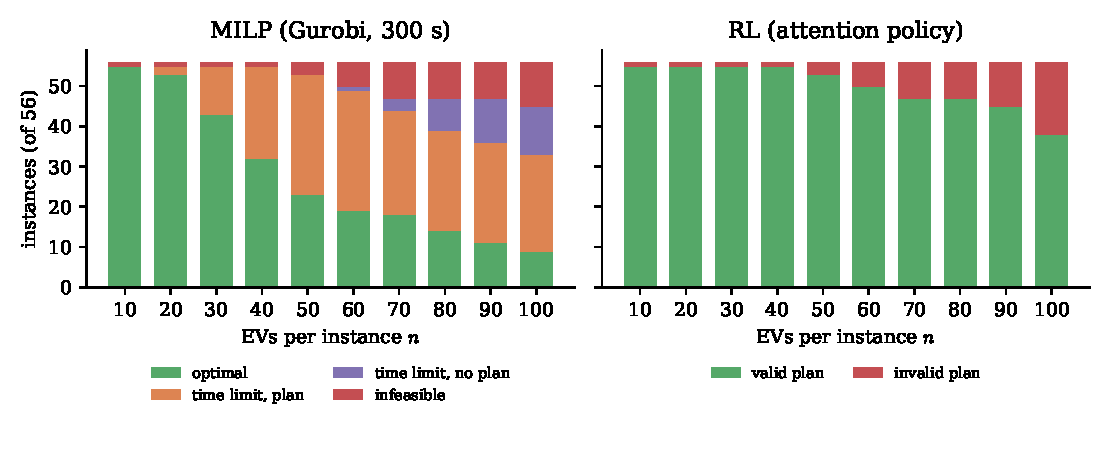
\includegraphics[width=0.95\textwidth]{figures/status_by_n.pdf}
\caption{Outcome of the 56 instances of each size for the two methods.}\end{figure}
\begin{table}[H]\centering
\small
\caption{How the 56 instances of each size ended, MILP (left) and RL (right).}\label{tab:statusn}
\begin{adjustbox}{max width=\textwidth}\begin{tabular}{lrrrrrrr}\toprule
$n$ & optimal & \shortstack{time limit\\with plan} & \shortstack{time limit\\no plan} & infeasible & \shortstack{RL\\valid} & \shortstack{RL\\invalid} & \shortstack{only RL\\valid} \\ \midrule
10 & 55 & 0 & 0 & 1 & 55 & 1 & 0 \\
20 & 53 & 2 & 0 & 1 & 55 & 1 & 0 \\
30 & 43 & 12 & 0 & 1 & 55 & 1 & 0 \\
40 & 32 & 23 & 0 & 1 & 55 & 1 & 0 \\
50 & 23 & 30 & 0 & 3 & 53 & 3 & 0 \\
60 & 19 & 30 & 1 & 6 & 50 & 6 & 1 \\
70 & 18 & 26 & 3 & 9 & 47 & 9 & 3 \\
80 & 14 & 25 & 8 & 9 & 47 & 9 & 8 \\
90 & 11 & 25 & 11 & 9 & 45 & 11 & 9 \\
100 & 9 & 24 & 12 & 11 & 38 & 18 & 5 \\
\midrule all & 277 & 197 & 35 & 51 & 500 & 60 & 26 \\
\bottomrule\end{tabular}\end{adjustbox}\end{table}

\begin{itemize}
  \item The MILP proves \MilpOptimal{} plans optimal, stops with a plan in \MilpTL{}, without one in \MilpTLnoPlan{}, and proves \MilpInfeasible{} instances infeasible. RL returns a valid plan in \RlValid{} instances.
  \item RL's \RlInvalid{} invalid plans are the \RlInvalidMilpInfeasible{} infeasible instances plus \RlInvalidMilpNoPlan{} where the MILP found no plan either; \RlInvalidShort{} of them are in the short-horizon families R1 and RC1. RL never fails where the MILP succeeds (\RlInvalidMilpValid{} such instances).
  \item In \RlOnly{} instances only RL has a plan; all were time-limit-without-plan instances of the MILP. \NeitherValid{} instances have no valid plan from either method.
\end{itemize}
\inshort{RL is valid wherever the MILP is, and in \RlOnly{} more instances; the \MilpInfeasible{} infeasible instances are beyond both.}

\subsection{How much dearer RL is}\label{sec:gap}
\begin{figure}[H]\centering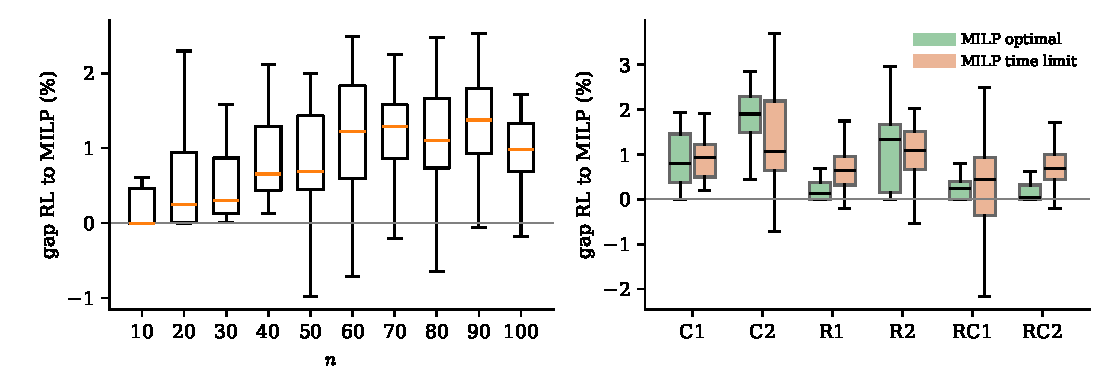
\includegraphics[width=0.95\textwidth]{figures/gap_baseline.pdf}
\caption{Gap of RL to the MILP by size (left) and by family, split by how the MILP ended (right).}\end{figure}
\begin{table}[H]\centering
\small
\caption{Gap of RL to the MILP on the instances valid for both, by size.}\label{tab:gapn}
\begin{adjustbox}{max width=\textwidth}\begin{tabular}{lrrrrrr}\toprule
$n$ & paired & mean (\%) & median (\%) & 90th pct (\%) & max (\%) & RL cheaper \\ \midrule
10 & 55 & 0.49 & 0.00 & 2.15 & 2.4 & 0 \\
20 & 55 & 0.60 & 0.24 & 1.69 & 2.8 & 0 \\
30 & 55 & 0.60 & 0.30 & 1.44 & 2.6 & 0 \\
40 & 55 & 0.81 & 0.65 & 1.76 & 3.0 & 2 \\
50 & 53 & 0.72 & 0.69 & 1.71 & 2.0 & 5 \\
60 & 49 & 1.03 & 1.23 & 2.07 & 3.7 & 6 \\
70 & 44 & 1.19 & 1.28 & 1.93 & 2.8 & 3 \\
80 & 39 & 1.17 & 1.11 & 2.26 & 4.8 & 4 \\
90 & 36 & 1.28 & 1.38 & 2.22 & 3.4 & 4 \\
100 & 33 & 1.02 & 0.99 & 1.69 & 4.8 & 4 \\
all & 474 & 0.85 & 0.76 & 2.00 & 4.8 & 28 \\
\bottomrule\end{tabular}\end{adjustbox}\end{table}

\begin{table}[H]\centering
\small
\caption{Gap of RL to the MILP by Solomon family, split by how the MILP ended.}\label{tab:gapfam}
\begin{adjustbox}{max width=\textwidth}\begin{tabular}{lrrrrrrr}\toprule
family & paired & mean (\%) & median (\%) & \shortstack{mean, MILP\\optimal (\%)} & \shortstack{mean, MILP\\time limit (\%)} & RL valid & only RL valid \\ \midrule
C1 & 89 & 0.84 & 0.84 & 0.86 & 0.78 & 90 & 1 \\
C2 & 79 & 1.66 & 1.80 & 1.79 & 1.34 & 79 & 0 \\
R1 & 75 & 0.38 & 0.31 & 0.26 & 0.53 & 89 & 14 \\
R2 & 110 & 1.16 & 1.26 & 1.12 & 1.21 & 110 & 0 \\
RC1 & 42 & 0.12 & 0.33 & 0.26 & 0.05 & 52 & 10 \\
RC2 & 79 & 0.48 & 0.46 & 0.17 & 0.68 & 80 & 1 \\
\bottomrule\end{tabular}\end{adjustbox}\end{table}

\begin{itemize}
  \item On the \BothValid{} instances valid for both, RL costs \GapMean\pct{} more on average (median \GapMedian\pct{}, 90th percentile \GapPninety\pct{}, at most \GapMax\pct{}); \RlWithinOne\pct{} of its plans are within 1\pct{} of the MILP.
  \item Against proven optima the gap is \GapOpt\pct{}; against time-limit plans \GapTL\pct{}. In \RlBetter{} instances RL is cheaper than the MILP, all of them time-limit plans; in \RlEqual{} it finds the same cost.
  \item The gap is largest in C2 and R2 (long horizons, many van decisions) and smallest in the short-horizon families R1 and RC1.
\end{itemize}
\inshort{RL is within about one per cent of the MILP on almost every instance; it beats unfinished MILP runs in \RlBetter{} instances.}

\subsection{Do the two methods take the same decisions?}\label{sec:agree}
\begin{table}[H]\centering
\small
\caption{Resource chosen for the same EV by the two methods (free-choice EVs of the paired instances).}\label{tab:agree}
\begin{adjustbox}{max width=\textwidth}\begin{tabular}{lrrrrrr}\toprule
segment & \shortstack{free-choice\\EVs} & \shortstack{both\\station} & \shortstack{MILP station\\RL van} & \shortstack{MILP van\\RL station} & \shortstack{both\\van} & same (\%) \\ \midrule
personal & 6095 & 4743 & 138 & 959 & 255 & 82.0 \\
commercial & 14125 & 13948 & 74 & 78 & 25 & 98.9 \\
all & 20220 & 18691 & 212 & 1037 & 280 & 93.8 \\
\bottomrule\end{tabular}\end{adjustbox}\end{table}

\begin{table}[H]\centering
\small
\caption{Composition of the objective and van use on the paired instances.}\label{tab:compm}
\begin{adjustbox}{max width=\textwidth}\begin{tabular}{lrrr}\toprule
term & MILP share of $Z$ (\%) & RL share of $Z$ (\%) & RL $-$ MILP (\% of MILP $Z$) \\ \midrule
$Z_1$ EV driving & 0.9 & 1.0 & +0.12 \\
$Z_2$ van driving & 2.4 & 2.3 & $-$0.08 \\
$Z_3$ van dispatch & 7.5 & 7.0 & $-$0.40 \\
$Z_4$ operator energy & 20.9 & 20.5 & $-$0.23 \\
$Z_5$ tariff & 39.3 & 38.5 & $-$0.44 \\
$Z_6$ time & 29.0 & 30.7 & +2.00 \\
vans used per instance & 2.19 & 2.08 &  \\
van seats used (\%) & 77.7 & 67.3 &  \\
van km per instance & 71.1 & 68.9 &  \\
\bottomrule\end{tabular}\end{adjustbox}\end{table}

\begin{itemize}
  \item \AgreeFree\pct{} of free-choice EVs get the same resource from both methods (\AgreeAll\pct{} of all EVs; stranded EVs always get a van). When both send an EV to a station, it is the same station in \AgreeStation\pct{} of cases.
  \item The disagreement is almost entirely about private cars: \MvanRfcsPersonal{} personal EVs get a van from the MILP but a station from RL, only \MfcsRvanPersonal{} the other way round. The methods agree on \AgreeCommercial\pct{} of commercial and \AgreePersonal\pct{} of personal free-choice EVs (Table~\ref{tab:agree}).
  \item RL dispatches about as many vans (\VansRl{} against \VansMilp{} per instance) but fills fewer seats. It saves a little dispatch cost ($Z_3$: \DZthreeRl{} points of $Z$) and pays much more in perceived time ($Z_6$: \DZsixRl{} points): the private owners it sends to stations lose the driver-free benefit.
\end{itemize}
\inshort{The methods agree on almost every commercial EV; RL's extra cost comes from the private owners it sends to stations instead of filling the van seats.}

\subsection{Who gets vans, by segment and income}
\begin{figure}[H]\centering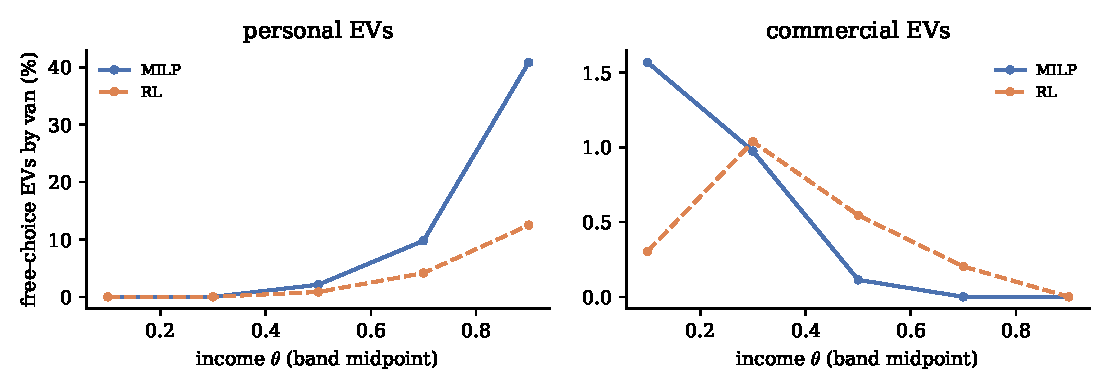
\includegraphics[width=0.9\textwidth]{figures/vanshare_methods.pdf}
\caption{Van share of free-choice EVs by income band, MILP (solid) and RL (dashed).}\end{figure}
\begin{table}[H]\centering
\small
\caption{Van share of free-choice EVs by segment and income band on the paired instances, MILP against RL (Wilson interval for the MILP share).}\label{tab:vsm}
\begin{adjustbox}{max width=\textwidth}\begin{tabular}{lrrrrr}\toprule
segment & income $\theta$ & free-choice EVs & MILP van (\%) & 95\,\% interval & RL van (\%) \\ \midrule
personal & 0.0--0.2 & 125 & 0.0 & [0.0, 3.0] & 0.0 \\
 & 0.2--0.4 & 608 & 0.0 & [0.0, 0.6] & 0.0 \\
 & 0.4--0.6 & 1181 & 2.1 & [1.4, 3.1] & 0.8 \\
 & 0.6--0.8 & 1668 & 9.8 & [8.4, 11.3] & 4.1 \\
 & 0.8--1.0 & 2513 & 40.8 & [38.9, 42.8] & 12.5 \\
commercial & 0.0--0.2 & 2297 & 1.6 & [1.1, 2.2] & 0.3 \\
 & 0.2--0.4 & 6363 & 1.0 & [0.8, 1.2] & 1.0 \\
 & 0.4--0.6 & 4398 & 0.1 & [0.0, 0.3] & 0.5 \\
 & 0.6--0.8 & 987 & 0.0 & [0.0, 0.4] & 0.2 \\
 & 0.8--1.0 & 80 & 0.0 & [0.0, 4.6] & 0.0 \\
\bottomrule\end{tabular}\end{adjustbox}\end{table}

\begin{table}[H]\centering
\small
\caption{Service per segment on the paired instances.}\label{tab:segm}
\begin{adjustbox}{max width=\textwidth}\begin{tabular}{lrrrr}\toprule
measure (per EV) & \shortstack{personal\\MILP} & \shortstack{personal\\RL} & \shortstack{commercial\\MILP} & \shortstack{commercial\\RL} \\ \midrule
mean station queue (min), station users & 0.41 & 0.38 & 1.58 & 2.53 \\
station users queueing (\%) & 2.8 & 3.0 & 9.4 & 12.8 \\
mean request to charged, downtime (min) & 60.6 & 61.0 & 64.3 & 66.3 \\
mean money paid (Rs) & 352 & 332 & 335 & 336 \\
mean perceived cost (Rs) & 662 & 691 & 582 & 590 \\
\bottomrule\end{tabular}\end{adjustbox}\end{table}

\begin{itemize}
  \item Both methods show the shape the theory predicts: private owners take vans more the richer they are (MILP: \VanPersTopMilp\pct{} in the top band), commercial drivers almost never (MILP \VanCommercialMilp\pct{}, RL \VanCommercialRl\pct{}).
  \item RL's curve for private owners has the same shape but a third of the height (\VanPersTopRl\pct{} in the top band).
  \item Commercial drivers queue longer at stations than private owners with both methods; RL's commercial queues are longer (\QueueComRl{} against \QueueComMilp{} min).
\end{itemize}
\inshort{Both methods reproduce ``segment before income''; RL under-uses vans for rich private owners.}

\subsection{Peak and off-peak: demand pressure}\label{sec:peak}
Demand pressure as defined in Section~\ref{sec:pressdef}: requests per charger during one mean charging time up to the EV's own request; low up to \PressLowCut, high above \PressHighCut.
\begin{figure}[H]\centering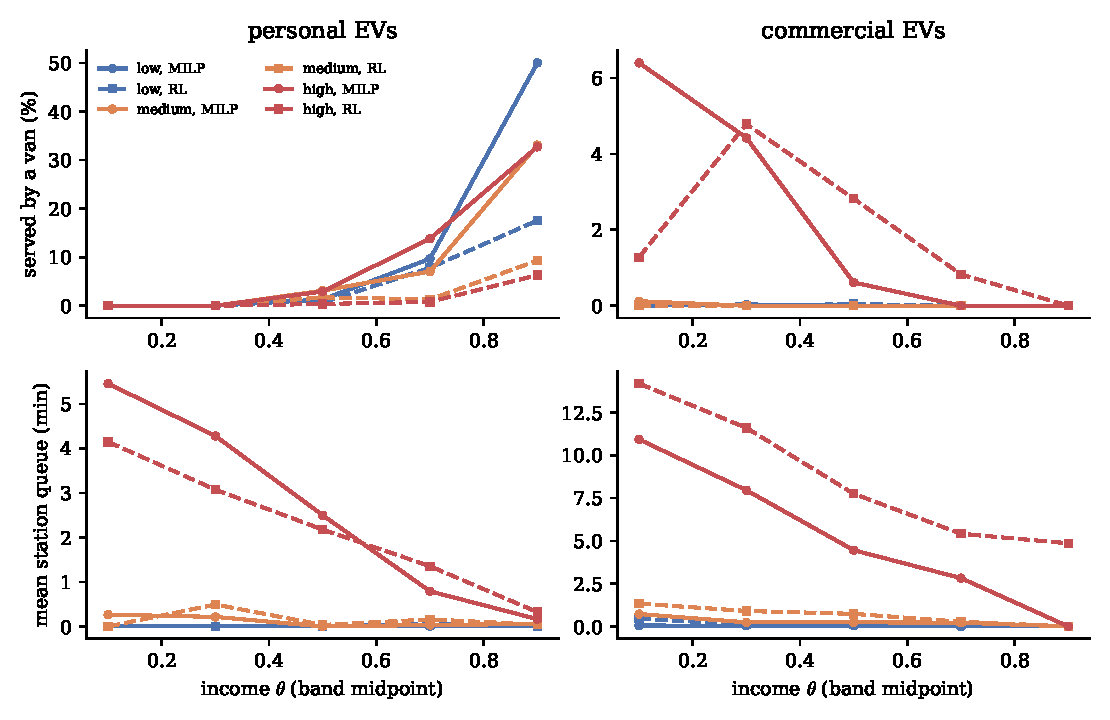
\includegraphics[width=0.92\textwidth]{figures/pressure_methods.pdf}
\caption{Van share (top) and mean station queue (bottom) by income band for low, medium and high pressure; MILP solid, RL dashed.}\end{figure}
\begin{table}[H]\centering
\small
\caption{Baseline, paired instances: van share and station queue of free-choice EVs by demand-pressure tercile and segment, MILP against RL.}\label{tab:pressm}
\begin{adjustbox}{max width=\textwidth}\begin{tabular}{lrrrrrrr}\toprule
segment & pressure & \shortstack{free-choice\\EVs} & \shortstack{MILP\\van (\%)} & \shortstack{RL\\van (\%)} & \shortstack{MILP station\\queue (min)} & \shortstack{RL station\\queue (min)} & \shortstack{MILP station users\\queueing (\%)} \\ \midrule
personal & low & 2816 & 23.4 & 9.4 & 0.00 & 0.02 & 0.0 \\
 & medium & 1914 & 17.1 & 4.8 & 0.06 & 0.12 & 1.1 \\
 & high & 1365 & 16.6 & 2.6 & 1.67 & 1.45 & 10.5 \\
commercial & low & 6664 & 0.0 & 0.0 & 0.04 & 0.16 & 0.7 \\
 & medium & 4464 & 0.0 & 0.0 & 0.33 & 0.89 & 3.8 \\
 & high & 2997 & 3.4 & 3.3 & 7.04 & 10.49 & 38.1 \\
\bottomrule\end{tabular}\end{adjustbox}\end{table}

\begin{table}[H]\centering
\scriptsize
\caption{Baseline: van share of free-choice EVs (\%, MILP / RL) by segment, pressure tercile and income band (paired instances).}\label{tab:pressband}
\begin{adjustbox}{max width=\textwidth}\begin{tabular}{llccccc}\toprule
segment & pressure & $\theta$ 0.0--0.2 & $\theta$ 0.2--0.4 & $\theta$ 0.4--0.6 & $\theta$ 0.6--0.8 & $\theta$ 0.8--1.0 \\ \midrule
personal & low & 0.0 / 0.0 & 0.0 / 0.0 & 1.3 / 0.6 & 9.7 / 7.8 & 50.0 / 17.5 \\
 & medium & 0.0 / 0.0 & 0.0 / 0.0 & 3.1 / 1.7 & 7.1 / 1.3 & 33.1 / 9.3 \\
 & high & 0.0 / 0.0 & 0.0 / 0.0 & 2.9 / 0.4 & 13.8 / 0.8 & 32.7 / 6.3 \\
commercial & low & 0.0 / 0.0 & 0.0 / 0.0 & 0.0 / 0.0 & 0.0 / 0.0 & 0.0 / 0.0 \\
 & medium & 0.1 / 0.0 & 0.0 / 0.0 & 0.0 / 0.0 & 0.0 / 0.0 & 0.0 / 0.0 \\
 & high & 6.4 / 1.3 & 4.4 / 4.8 & 0.6 / 2.8 & 0.0 / 0.8 & 0.0 / 0.0 \\
\bottomrule\end{tabular}\end{adjustbox}\end{table}

\begin{table}[H]\centering
\scriptsize
\caption{Baseline: mean station queue of free-choice station users (min, MILP / RL) by segment, pressure tercile and income band.}\label{tab:pressbandq}
\begin{adjustbox}{max width=\textwidth}\begin{tabular}{llccccc}\toprule
segment & pressure & $\theta$ 0.0--0.2 & $\theta$ 0.2--0.4 & $\theta$ 0.4--0.6 & $\theta$ 0.6--0.8 & $\theta$ 0.8--1.0 \\ \midrule
personal & low & 0.0 / 0.0 & 0.0 / 0.0 & 0.0 / 0.0 & 0.0 / 0.1 & 0.0 / 0.0 \\
 & medium & 0.3 / 0.0 & 0.2 / 0.5 & 0.0 / 0.0 & 0.0 / 0.2 & 0.1 / 0.0 \\
 & high & 5.5 / 4.1 & 4.3 / 3.1 & 2.5 / 2.2 & 0.8 / 1.4 & 0.2 / 0.3 \\
commercial & low & 0.1 / 0.4 & 0.0 / 0.1 & 0.0 / 0.1 & 0.0 / 0.1 & 0.0 / 0.0 \\
 & medium & 0.7 / 1.3 & 0.2 / 0.9 & 0.2 / 0.7 & 0.2 / 0.3 & 0.0 / 0.0 \\
 & high & 10.9 / 14.2 & 8.0 / 11.6 & 4.5 / 7.8 & 2.8 / 5.4 & 0.0 / 4.9 \\
\bottomrule\end{tabular}\end{adjustbox}\end{table}

\begin{itemize}
  \item \textbf{Queues are a peak phenomenon.} Commercial station users queue \PQueueCommercialLowMilp{} min at low and \PQueueCommercialHighMilp{} min at high pressure (MILP); at high pressure the poorest commercial drivers queue \PQueueComHighPoorMilp{} min, the richest private owners \PQueuePersHighRichMilp{} min.
  \item \textbf{Commercial EVs take vans only at peak}, as formulation 4 predicts (queues, not income, push them to vans): \PVanCommercialLowMilp\pct{} at low, \PVanCommercialHighMilp\pct{} at high pressure. \ComVanUsersHighShare\pct{} of the \ComVanUsers{} commercial van users are in the high tercile, and they are poorer than commercial station users (mean $\theta$ \ComVanUsersTheta{} against \ComFcsUsersTheta).
  \item \textbf{Private owners take vans mostly off-peak}: \PVanPersonalLowMilp\pct{} at low, \PVanPersonalHighMilp\pct{} at high pressure. At peak the seats are shared with stranded EVs and commercial EVs facing queues.
  \item \textbf{RL reproduces the peak behaviour of commercial EVs} (\PVanCommercialHighRl\pct{} at high pressure, none below) but not that of private owners: its van share falls from \PVanPersonalLowRl\pct{} to \PVanPersonalHighRl\pct{}, and its commercial queues at peak are longer (\PQueueCommercialHighRl{} min).
  \item \textbf{Caveat 1: the peak label.} Formulation 4's label (load above the instance median) calls a request tied with the start-of-period burst off-peak; \OffHighShare\pct{} of free-choice EVs are ``off-peak'' but in the high pressure tercile, and all \ComVanOffPeak{} commercial van users are labelled off-peak. The terciles are used here for that reason; with the median label the commercial share would read \PPeakVanCommercialMilp\pct{} at peak and \POffVanCommercialMilp\pct{} off-peak, which is misleading.
  \item \textbf{Caveat 2: only time-limit plans have peaks.} All \ComVanUsers{} commercial van users are in time-limit plans (\ComVanInOptimal{} in proven-optimal plans); the \ComHighNOpt{} high-pressure commercial station users of optimal plans do not queue (\ComHighQueueOpt{} min against \ComHighQueueTL{} min in time-limit plans). Congestion occurs only in the large instances the MILP does not finish, so the peak behaviour cannot be confirmed on proven optima. That RL, an independent method, finds the same commercial van share at peak supports it being a property of the model rather than of the unfinished search.
\end{itemize}
\inshort{At peak, queues push poor commercial drivers to vans and private owners lose their seats; RL reproduces the commercial part. Congestion exists only in instances the MILP does not finish, so this is confirmed by two methods but not by proofs.}

\subsection{Time}
\begin{figure}[H]\centering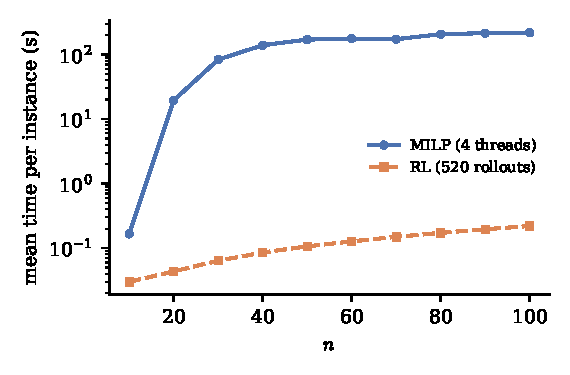
\includegraphics[width=0.5\textwidth]{figures/time_methods.pdf}
\caption{Mean time per instance (log scale).}\end{figure}
The MILP needs \MilpSolveMean{}\,s per instance on average (about \MilpCPUh{} core-hours for the 560), RL \RlSolveMean{}\,s, \SpeedUp{} times less; RL's one-off training took \RlTrainMin{} minutes on a GPU.
\inshort{RL answers in a tenth of a second; the MILP needs minutes from $n\approx40$ on.}

%=====================================================================
\section{Infrastructure utilisation}\label{sec:util}
Measured with \code{common/infra.py} on the \BothValid{} paired baseline instances. As in the MILP and RL reports, every utilisation is the mean of per-instance (or per-van) shares; a value that divides sums over instances is marked \emph{pooled}. Capacities: every gun of 22\,kW and every van of 30\,kW is available during $[0,T]$; a van has 6 seats and a 150\,kWh battery. An instance asks for \UKwhPerInst\,kWh on average.
\begin{table}[H]\centering
\small
\caption{Infrastructure utilisation on the 474 paired baseline instances (24 guns of 22\,kW, 5 vans of 30\,kW, 6 seats, 150\,kWh, over $[0,T]$). Means of per-instance (guns, energy) and per-van shares; rows marked pooled divide sums over instances.}\label{tab:utilm}
\begin{adjustbox}{max width=\textwidth}\begin{tabular}{lrrr}\toprule
measure & MILP & RL & RL $-$ MILP \\ \midrule
gun utilisation, mean over instances (\% of $G\,T$) & 12.8 & 13.3 & +0.5 \\
gun utilisation, pooled over instances (\%) & 7.2 & 7.5 & +0.3 \\
90th percentile of gun utilisation (\%) & 34.6 & 35.9 & +1.3 \\
busiest gun (\%) & 91.4 & 92.4 & +1.1 \\
idle guns per instance (of 24) & 7.0 & 6.1 & $-$0.8 \\
guns never used (\%) & 29.0 & 25.6 & $-$3.5 \\
energy delivered by vans (\% of the instance's kWh) & 20.1 & 16.9 & $-$3.2 \\
energy delivered by vans, pooled (\% of all kWh) & 19.7 & 16.5 & $-$3.2 \\
installed-capacity utilisation (\%) & 12.4 & 12.4 & $-$0.0 \\
vans dispatched per instance & 2.19 & 2.08 & $-$0.12 \\
fleet use (dispatched / $M$, \%) & 43.9 & 41.6 & $-$2.3 \\
seat use of dispatched vans (\%) & 79.0 & 69.4 & $-$9.6 \\
vans with every seat taken (\%) & 48.1 & 19.4 & $-$28.7 \\
battery drawn (\% of $B$) & 71.1 & 63.5 & $-$7.6 \\
vans drawing $>$90\,\% of $B$ (\%) & 22.2 & 14.5 & $-$7.7 \\
time on the road (\% of $T$) & 68.4 & 68.6 & +0.2 \\
time charging EVs (\% of $T$) & 24.8 & 22.0 & $-$2.8 \\
van power capacity used (\% of $P^{\mathrm M}T$) & 24.8 & 22.0 & $-$2.8 \\
on-road time spent charging (\%) & 35.4 & 31.7 & $-$3.7 \\
on-road time spent driving (\%) & 26.3 & 26.7 & +0.3 \\
on-road time idle or waiting (\%) & 38.2 & 41.6 & +3.4 \\
on-road time idle or waiting, pooled (\%) & 59.7 & 63.4 & +3.7 \\
\bottomrule\end{tabular}\end{adjustbox}\end{table}

\begin{figure}[H]\centering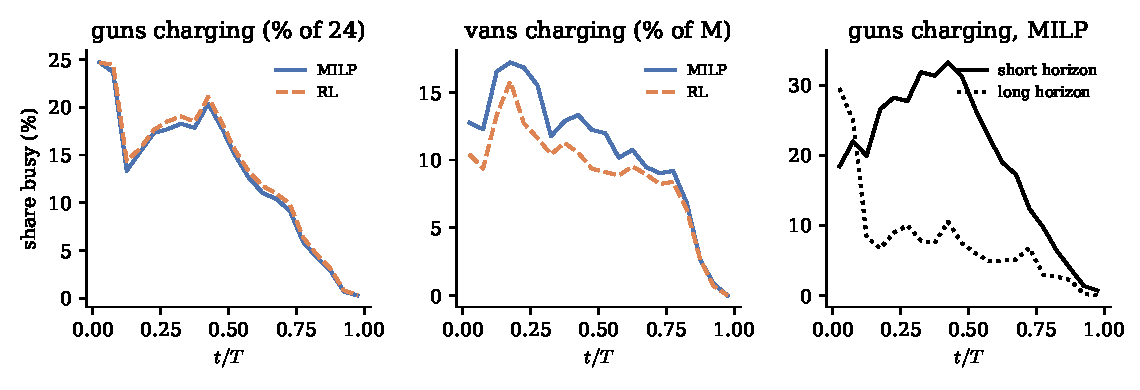
\includegraphics[width=0.98\textwidth]{figures/util_profile.pdf}
\caption{Share of guns and vans charging over the period (mean over instances): MILP solid, RL dashed; right: short against long horizons (MILP).}\end{figure}
\begin{table}[H]\centering
\small
\caption{Utilisation by family, MILP / RL (paired baseline instances; means of per-instance and per-van shares).}\label{tab:utilfam}
\begin{adjustbox}{max width=\textwidth}\begin{tabular}{lrcccccccc}\toprule
family & inst. & \shortstack{gun time\\(\%)} & \shortstack{idle guns\\(of 24)} & \shortstack{van share\\of kWh (\%)} & \shortstack{fleet\\use (\%)} & \shortstack{seats\\(\%)} & \shortstack{battery\\(\%)} & \shortstack{on the road\\(\% of $T$)} & \shortstack{installed\\capacity (\%)} \\ \midrule
C1 & 89 & 8.0 / 8.5 & 9.4 / 8.6 & 21.0 / 17.6 & 44 / 42 & 95 / 80 & 83 / 69 & 65 / 68 & 7.9 / 7.9 \\
C2 & 79 & 3.0 / 3.1 & 8.3 / 6.8 & 21.5 / 16.6 & 38 / 36 & 92 / 78 & 91 / 80 & 63 / 66 & 2.9 / 2.9 \\
R1 & 75 & 26.9 / 27.7 & 5.7 / 5.5 & 23.3 / 21.5 & 47 / 45 & 51 / 46 & 47 / 44 & 87 / 84 & 26.2 / 26.2 \\
R2 & 110 & 9.2 / 9.6 & 4.9 / 3.8 & 19.6 / 15.8 & 42 / 40 & 94 / 81 & 73 / 63 & 62 / 62 & 8.8 / 8.8 \\
RC1 & 42 & 30.0 / 31.4 & 6.3 / 6.1 & 14.1 / 11.2 & 49 / 41 & 41 / 37 & 43 / 40 & 85 / 84 & 28.1 / 28.1 \\
RC2 & 79 & 10.7 / 11.0 & 7.4 / 6.5 & 18.4 / 16.5 & 48 / 45 & 81 / 75 & 78 / 75 & 57 / 56 & 10.4 / 10.4 \\
\bottomrule\end{tabular}\end{adjustbox}\end{table}

\begin{table}[H]\centering
\small
\caption{Utilisation by instance size (paired baseline instances; means of per-instance shares).}\label{tab:utiln}
\begin{adjustbox}{max width=\textwidth}\begin{tabular}{lrrrrrrrr}\toprule
$n$ & inst. & \shortstack{gun time\\MILP (\%)} & \shortstack{gun time\\RL (\%)} & \shortstack{idle guns\\MILP} & \shortstack{van kWh\\MILP (\%)} & \shortstack{van kWh\\RL (\%)} & \shortstack{fleet use\\MILP (\%)} & \shortstack{installed cap.\\MILP (\%)} \\ \midrule
10 & 55 & 3.5 & 3.5 & 18.5 & 23.7 & 20.3 & 18 & 3.4 \\
20 & 55 & 6.9 & 7.0 & 13.6 & 22.9 & 19.7 & 24 & 6.9 \\
30 & 55 & 11.0 & 11.1 & 9.5 & 17.0 & 14.6 & 28 & 10.3 \\
40 & 55 & 15.0 & 15.5 & 6.2 & 17.1 & 14.0 & 36 & 13.9 \\
50 & 53 & 17.1 & 17.9 & 4.8 & 18.9 & 16.3 & 46 & 16.5 \\
60 & 49 & 18.2 & 19.1 & 4.1 & 20.9 & 16.9 & 56 & 17.7 \\
70 & 44 & 17.4 & 18.2 & 2.4 & 19.6 & 16.3 & 58 & 17.0 \\
80 & 39 & 14.8 & 15.6 & 1.6 & 20.4 & 16.5 & 64 & 14.5 \\
90 & 36 & 12.8 & 13.4 & 1.0 & 20.8 & 17.3 & 69 & 12.5 \\
100 & 33 & 14.5 & 15.0 & 0.3 & 19.2 & 16.6 & 69 & 14.0 \\
\bottomrule\end{tabular}\end{adjustbox}\end{table}

\begin{figure}[H]\centering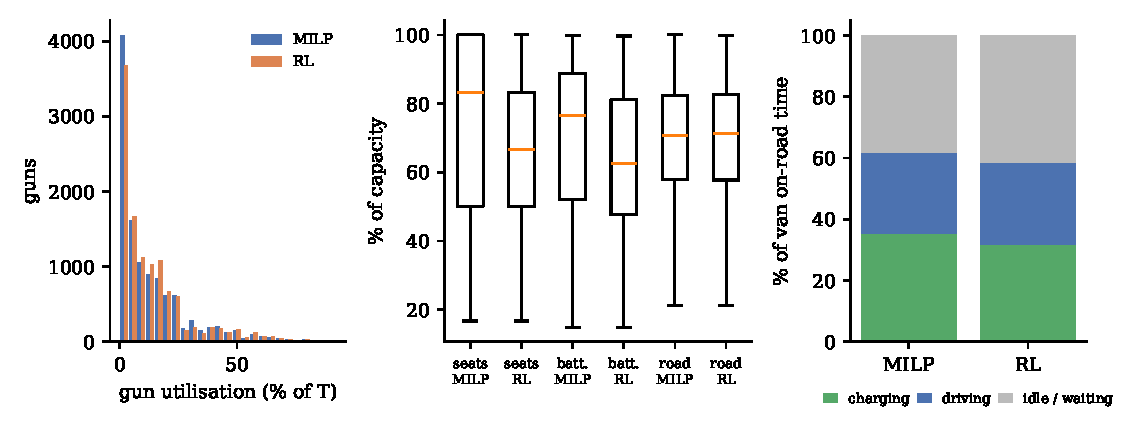
\includegraphics[width=0.98\textwidth]{figures/util_dists.pdf}
\caption{Gun utilisation of every gun (left), van seats, battery and time on the road (middle), and how vans spend their time on the road (right).}\end{figure}

\subsection{Stations and guns}
\begin{itemize}
  \item On average a gun charges during \UGunMilp\pct{} of the period (MILP; RL \UGunRl\pct; mean of per-instance shares; pooled over all instances \UGunPooledMilp\pct, because long horizons weigh more); the busiest gun of an instance reaches \UGunMaxMilp\pct{}, the 90th percentile \UGunPninetyMilp\pct. \UIdleGunShareMilp\pct{} of guns are never used (\UIdleGunsMilp{} per instance; \UIdleGunsMilpNten{} at $n=10$, \UIdleGunsMilpNhundred{} at $n=100$).
  \item The busy profile follows the demand: at most \UPeakGunsBusy\pct{} of guns charge at once, at the start of the period ($t/T\approx$ \UPeakGunsAt), when the burst of requests at $t=0$ arrives; after $0.75\,T$ only \ULateGunsBusy\pct{}.
  \item By family, the short horizons are the busiest (R1 \UGunFamRone\pct{}, RC1 \UGunFamRCone\pct) and C2 the least (\UGunFamCtwo\pct): the same demand in a much shorter period.
\end{itemize}
\inshort{Stations have far more capacity than the demand needs on average; they are scarce only in the start-of-period burst and in the short-horizon families.}

\subsection{Vans}
\begin{itemize}
  \item \UVansUsedMilp{} of the 5 vans leave per instance (fleet use \UFleetMilp\pct). A dispatched van fills \USeatMilp\pct{} of its seats (\UFullMilp\pct{} are full) and draws \UBatteryMilp\pct{} of its battery (\UBninetyMilp\pct{} draw more than 90\pct).
  \item A van is on the road \UOnRoadMilp\pct{} of the period but charges only \UChargeMilp\pct{} of it, which is also the share of its power capacity used. Of its on-road time, \UChargeVanMilp\pct{} is charging, \UDriveVanMilp\pct{} driving and \UIdleVanMilp\pct{} waiting for the next EV's request (means over vans; pooled over all vans the waiting share is \UIdleVanPooledMilp\pct, because the long-horizon vans wait longest).
  \item In the short horizons vans are on the road most of the period (R1 \UOnRoadFamRone\pct) with few seats used (R1 \USeatFamRone\pct): they run out of time; in the long horizons they fill their seats (C1 \USeatFamCone\pct).
  \item RL leaves the seats emptier (\USeatRl\pct, \UFullRl\pct{} full) and its vans carry less energy (\UVanEnergyRl\pct{} of an instance's kWh against \UVanEnergyMilp\pct).
\end{itemize}
\inshort{Seats are the van resource in use; battery, power and time are mostly spare, and over a third of a van's time on the road is spent waiting for requests.}

\subsection{The system}
\begin{itemize}
  \item Vans deliver \UVanEnergyMilp\pct{} of an instance's energy on average (RL \UVanEnergyRl\pct; pooled over all instances \UVanEnergyPooledMilp\pct), stations the rest.
  \item The installed capacity (24 guns and 5 vans over $[0,T]$) is used at \USystemMilp\pct{} on average (\USystemMilpNhundred\pct{} at $n=100$). Every EV is fully charged in every valid plan, so this number depends only on the data and the fleet, never on the method: it is the same for the MILP and RL.
\end{itemize}
\inshort{The network is sized for the burst, not for the average: about one eighth of the installed capacity is used, and how it is shared between stations and vans is the only thing a plan changes.}

\part{The experiments}
\section{First check: every variant moves the optimum the right way}\label{sec:direction}
A cost coefficient that rises (or a capacity that falls) cannot lower the exact optimum, because every plan of the baseline remains possible and none becomes cheaper. On the instances optimal in both runs this must hold exactly.
\begin{table}[H]\centering
\scriptsize
\caption{Checks of every variant. Left: the exact optimum on instances optimal in both MILP runs (direction check). Right: RL against the MILP of the same variant; last column: correlation over instances of the MILP and the retrained-RL change of $Z$.}\label{tab:direction}
\begin{adjustbox}{max width=\textwidth}\begin{tabular}{lrrrrrrrrr}\toprule
variant & \shortstack{expected\\sign} & \shortstack{optimal\\pairs} & \shortstack{mean $\Delta Z$\\optimal (\%)} & \shortstack{unchanged\\($\le$0.01\,\%)} & violations & \shortstack{RL$_{\mathrm{rt}}$ effect\\$-$ MILP effect} & \shortstack{gap to MILP\\zero-shot (\%)} & \shortstack{gap to MILP\\retrained (\%)} & \shortstack{corr.\ of\\$\Delta Z$} \\ \midrule
personal $c^{\mathrm C,1}=7.5$ & $-$ & 275 & $-$2.19 & 5 & 0 & $-$0.25 & 0.56 & 0.56 & 0.76 \\
personal $c^{\mathrm C,1}=12.5$ & $+$ & 252 & +1.95 & 12 & 0 & +0.30 & 1.22 & 1.14 & 0.75 \\
commercial $\omega^{1}=4.5$ & $-$ & 275 & $-$2.51 & 0 & 0 & +0.14 & 0.82 & 0.98 & 0.56 \\
commercial $\omega^{1}=7.5$ & $+$ & 275 & +2.50 & 0 & 0 & +0.09 & 0.83 & 0.86 & 0.49 \\
personal $\mu^{0}=1.125$ & $-$ & 273 & $-$1.30 & 0 & 0 & +0.13 & 0.92 & 0.95 & 0.43 \\
personal $\mu^{0}=1.875$ & $+$ & 276 & +1.30 & 0 & 0 & +0.03 & 0.80 & 0.84 & 0.44 \\
commercial $\mu^{0}=1.125$ & $-$ & 272 & $-$6.45 & 0 & 0 & +0.14 & 0.87 & 0.91 & 0.79 \\
commercial $\mu^{0}=1.875$ & $+$ & 275 & +6.46 & 0 & 0 & $-$0.10 & 0.80 & 0.79 & 0.82 \\
$p^{\mathrm M}=15$ & $-$ & 225 & $-$4.45 & 7 & 0 & +0.41 & 1.31 & 1.25 & 0.81 \\
$p^{\mathrm M}=35$ & $+$ & 276 & +4.07 & 7 & 0 & $-$0.19 & 0.58 & 0.63 & 0.79 \\
3 vans & $+$ & 275 & +0.00 & 275 & 0 & +0.13 & 0.91 & 0.96 & 0.00 \\
7 vans & $-$ & 273 & $-$0.00 & 273 & 0 & $-$0.01 & 0.84 & 0.81 & $-$0.17 \\
4 seats per van & $+$ & 275 & +1.30 & 108 & 0 & $-$0.20 & 0.69 & 0.65 & 0.74 \\
8 seats per van & $-$ & 263 & $-$0.16 & 188 & 0 & +0.15 & 0.86 & 0.98 & 0.23 \\
battery 200 kWh & $-$ & 274 & $-$0.04 & 240 & 0 & $-$0.07 & 0.84 & 0.77 & 0.08 \\
\bottomrule\end{tabular}\end{adjustbox}\end{table}

\begin{itemize}
  \item Over \DirPairs{} pairs of optimal plans there are \DirBad{} violations: the runs are consistent with the model.
  \item Several variants leave the optimum unchanged in many optimal pairs (column ``unchanged''): with 3 or 7 vans every optimal pair is unchanged, with the 200\,kWh battery most of them. These capacities do not bind in the instances the MILP solves to optimality.
  \item RL's gap to the MILP of the same variant stays between \GapVarMin\pct{} and \GapVarMax\pct{}, close to the baseline's \GapMean\pct{}. The correlation of the instance-level effects is high where the effect is large (E6 commercial, E1, E5 personal) and near zero where the MILP effect is zero (vans, battery).
\end{itemize}
\inshort{\DirBad{} violations in \DirPairs{} optimal pairs; the experiments measure the model, not solver noise.}

\clearpage
\section{E5: value of charging time at \texorpdfstring{$\theta=1$}{theta=1}}\label{sec:e5}
\begin{table}[H]\centering
\scriptsize
\caption{E5: every variant against its own baseline, for the three runs (paired instances; van shares and vans used: baseline $\to$ variant on the same paired instances).}\label{tab:expE5}
\begin{adjustbox}{max width=\textwidth}\begin{tabular}{llrrrrrrrrrr}\toprule
variant & method & valid & paired & \shortstack{newly valid\\/ lost} & \shortstack{mean\\$\Delta Z$ (\%)} & \shortstack{median\\$\Delta Z$ (\%)} & \shortstack{operator\\(\%)} & \shortstack{customers\\(\%)} & \shortstack{van share\\personal (\%)} & \shortstack{van share\\commercial (\%)} & vans used \\ \midrule
personal $c^{\mathrm C,1}=7.5$ & MILP & 473 & 472 & +1/$-$2 & $-$2.21 & $-$2.20 & $-$1.15 & $-$2.59 & 19.9$\to$14.0 & 0.72$\to$0.82 & 2.18$\to$2.13 \\
 & RL zero-shot & 499 & 499 & +0/$-$1 & $-$2.49 & $-$2.54 & $-$0.21 & $-$3.45 & 6.7$\to$5.5 & 0.93$\to$0.92 & 2.20$\to$2.20 \\
 & RL retrained & 500 & 499 & +1/$-$1 & $-$2.46 & $-$2.56 & $-$0.59 & $-$3.24 & 6.7$\to$3.9 & 0.93$\to$0.83 & 2.20$\to$2.19 \\
personal $c^{\mathrm C,1}=12.5$ & MILP & 473 & 472 & +1/$-$2 & +2.08 & +1.99 & +2.75 & +1.84 & 19.9$\to$29.4 & 0.73$\to$0.67 & 2.18$\to$2.37 \\
 & RL zero-shot & 502 & 500 & +2/$-$0 & +2.45 & +2.49 & +0.31 & +3.36 & 6.7$\to$8.0 & 0.94$\to$0.84 & 2.21$\to$2.23 \\
 & RL retrained & 500 & 500 & +0/$-$0 & +2.38 & +2.46 & +0.93 & +3.02 & 6.7$\to$11.7 & 0.94$\to$0.56 & 2.21$\to$2.26 \\
commercial $\omega^{1}=4.5$ & MILP & 472 & 471 & +1/$-$3 & $-$2.67 & $-$2.66 & $-$0.17 & $-$3.80 & 19.9$\to$19.6 & 0.72$\to$0.67 & 2.18$\to$2.17 \\
 & RL zero-shot & 500 & 499 & +1/$-$1 & $-$2.72 & $-$2.71 & $-$0.13 & $-$3.86 & 6.7$\to$6.5 & 0.93$\to$0.85 & 2.20$\to$2.19 \\
 & RL retrained & 500 & 499 & +1/$-$1 & $-$2.52 & $-$2.56 & +0.17 & $-$3.70 & 6.7$\to$7.6 & 0.91$\to$0.57 & 2.20$\to$2.23 \\
commercial $\omega^{1}=7.5$ & MILP & 475 & 472 & +3/$-$2 & +2.66 & +2.65 & +0.26 & +3.81 & 19.9$\to$19.6 & 0.73$\to$0.68 & 2.18$\to$2.20 \\
 & RL zero-shot & 500 & 500 & +0/$-$0 & +2.72 & +2.71 & +0.26 & +3.82 & 6.7$\to$6.9 & 0.94$\to$0.93 & 2.21$\to$2.24 \\
 & RL retrained & 499 & 499 & +0/$-$1 & +2.75 & +2.69 & +0.14 & +3.92 & 6.7$\to$7.0 & 0.91$\to$0.79 & 2.20$\to$2.22 \\
\bottomrule\end{tabular}\end{adjustbox}\end{table}

\begin{figure}[H]\centering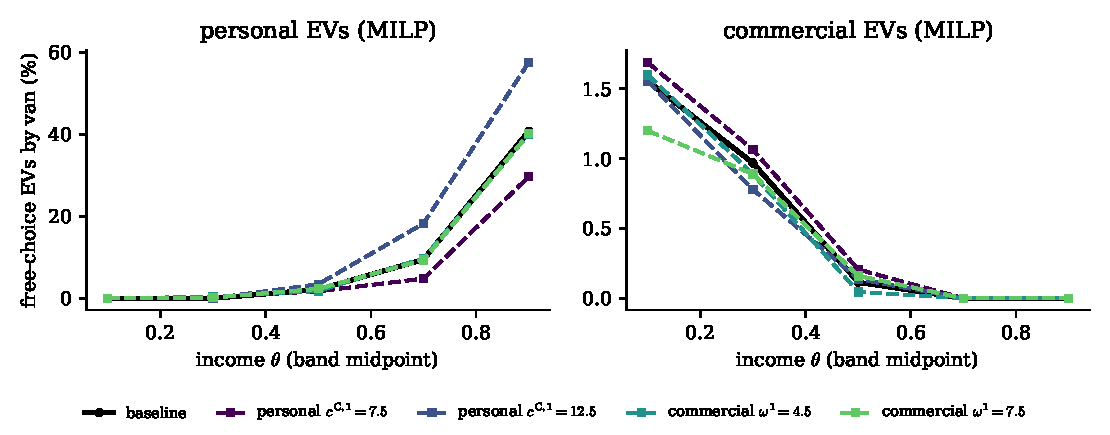
\includegraphics[width=0.92\textwidth]{figures/vanshare_E5.pdf}
\caption{E5, MILP: van share by income band, baseline and variants.}\end{figure}
\begin{table}[H]\centering
\small
\caption{E5, MILP: van share of free-choice EVs (\%) by segment and income band, on the 470 instances valid in the baseline and every variant.}\label{tab:bandE5}
\begin{adjustbox}{max width=\textwidth}\begin{tabular}{lrrrrrr}\toprule
segment & income $\theta$ & baseline & personal $c^{\mathrm C,1}=7.5$ & personal $c^{\mathrm C,1}=12.5$ & commercial $\omega^{1}=4.5$ & commercial $\omega^{1}=7.5$ \\ \midrule
personal & 0.0--0.2 & 0.0 & 0.0 & 0.0 & 0.0 & 0.0 \\
 & 0.2--0.4 & 0.0 & 0.3 & 0.0 & 0.3 & 0.2 \\
 & 0.4--0.6 & 2.1 & 1.7 & 3.4 & 1.8 & 2.3 \\
 & 0.6--0.8 & 9.5 & 4.8 & 18.2 & 9.8 & 9.3 \\
 & 0.8--1.0 & 40.7 & 29.6 & 57.5 & 40.0 & 40.1 \\
commercial & 0.0--0.2 & 1.6 & 1.7 & 1.6 & 1.6 & 1.2 \\
 & 0.2--0.4 & 1.0 & 1.1 & 0.8 & 0.9 & 0.9 \\
 & 0.4--0.6 & 0.1 & 0.2 & 0.1 & 0.0 & 0.2 \\
 & 0.6--0.8 & 0.0 & 0.0 & 0.0 & 0.0 & 0.0 \\
 & 0.8--1.0 & 0.0 & 0.0 & 0.0 & 0.0 & 0.0 \\
\bottomrule\end{tabular}\end{adjustbox}\end{table}

\begin{table}[H]\centering
\scriptsize
\caption{E5, MILP: change of the perceived cost (\%) and of the money paid (Rs) per EV, by segment and income band (all EVs of the paired instances, stranded EVs included: they always pay the van tariff).}\label{tab:eqE5}
\begin{adjustbox}{max width=\textwidth}\begin{tabular}{llrrrrrrrr}\toprule
segment & income $\theta$ & \shortstack{personal $c^{\mathrm C,1}=7.5$\\perceived (\%)} & \shortstack{paid\\(Rs)} & \shortstack{personal $c^{\mathrm C,1}=12.5$\\perceived (\%)} & \shortstack{paid\\(Rs)} & \shortstack{commercial $\omega^{1}=4.5$\\perceived (\%)} & \shortstack{paid\\(Rs)} & \shortstack{commercial $\omega^{1}=7.5$\\perceived (\%)} & \shortstack{paid\\(Rs)} \\ \midrule
personal & 0.0--0.2 & $-$2.0 & $-$1 & +2.5 & $-$1 & +0.8 & $-$1 & +1.5 & +0 \\
 & 0.2--0.4 & $-$4.9 & +1 & +5.8 & +0 & $-$0.3 & +1 & +0.7 & +1 \\
 & 0.4--0.6 & $-$8.3 & $-$1 & +8.3 & +2 & $-$0.2 & $-$1 & +0.4 & +1 \\
 & 0.6--0.8 & $-$10.3 & $-$8 & +8.2 & +15 & $-$0.3 & +0 & +0.4 & $-$1 \\
 & 0.8--1.0 & $-$8.0 & $-$18 & +0.9 & +31 & $-$0.1 & $-$1 & +0.5 & $-$1 \\
commercial & 0.0--0.2 & +0.1 & +0 & $-$0.2 & $-$0 & $-$2.7 & $-$0 & +2.0 & $-$1 \\
 & 0.2--0.4 & +0.1 & +0 & $-$0.2 & $-$0 & $-$4.7 & $-$0 & +4.6 & +0 \\
 & 0.4--0.6 & +0.2 & +0 & $-$0.0 & $-$0 & $-$7.8 & $-$0 & +7.8 & +0 \\
 & 0.6--0.8 & +0.1 & $-$0 & +0.1 & $-$0 & $-$10.2 & +0 & +10.2 & +0 \\
 & 0.8--1.0 & +1.8 & +1 & $-$1.4 & $-$1 & $-$13.7 & +0 & +14.7 & +0 \\
\bottomrule\end{tabular}\end{adjustbox}\end{table}

\begin{itemize}
  \item \textbf{Personal $c^{\mathrm C,1}$ moves the van share of private owners strongly}: \VanPBEfivePersLoMilp\pct{} $\to$ \VanPEfivePersLoMilp\pct{} at 7.5 and \VanPBEfivePersHiMilp\pct{} $\to$ \VanPEfivePersHiMilp\pct{} at 12.5 (MILP); the change happens in the two top income bands, where the threshold lies. $Z$ moves \dZEfivePersLoMilp\pct{} / \dZEfivePersHiMilp\pct{}, mostly through the private owners' perceived cost (\CcPersEfivePersLoMilp\pct{} / \CcPersEfivePersHiMilp\pct).
  \item \textbf{The commercial downtime rate $\omega^1$ moves $Z$ more} (\dZEfiveComLoMilp\pct{} / \dZEfiveComHiMilp\pct), entirely through the commercial perceived cost (\CcComEfiveComLoMilp\pct{} / \CcComEfiveComHiMilp\pct), \textbf{but not the van share}: commercial \VanCBEfiveComHiMilp\pct{} $\to$ \VanCEfiveComHiMilp\pct{} at 7.5.
  \item \textbf{The peak prediction is not confirmed} (Section~\ref{sec:e5peak}).
  \item RL reproduces the effects on $Z$ (\dZEfivePersHiRt\pct{} and \dZEfiveComHiRt\pct{} for the two high variants, retrained) and the direction of the personal van share (\VanPBEfivePersHiRt\pct{} $\to$ \VanPEfivePersHiRt\pct{}), with a smaller amplitude.
\end{itemize}

\subsection{Does a higher downtime rate push commercial EVs to vans at peak?}\label{sec:e5peak}
\begin{table}[H]\centering
\scriptsize
\caption{Every variant at low and at high demand pressure (MILP unless stated; changes against the baseline on the paired instances): van share of free-choice EVs in percentage points and mean station queue of commercial station users in minutes.}\label{tab:pressexp}
\begin{adjustbox}{max width=\textwidth}\begin{tabular}{lrrrrrrr}\toprule
variant & \shortstack{low: van\\personal} & \shortstack{low: van\\commercial} & \shortstack{low: queue\\commercial} & \shortstack{high: van\\personal} & \shortstack{high: van\\commercial} & \shortstack{high: queue\\commercial} & \shortstack{RL$_{\mathrm{rt}}$ high: van\\commercial} \\ \midrule
personal $c^{\mathrm C,1}=7.5$ & $-$5.8 & +0.00 & $-$0.00 & $-$5.3 & +0.48 & +0.23 & $-$0.51 \\
personal $c^{\mathrm C,1}=12.5$ & +10.8 & $-$0.02 & +0.01 & +5.7 & $-$0.27 & $-$0.64 & $-$1.50 \\
commercial $\omega^{1}=4.5$ & $-$0.6 & +0.00 & +0.00 & $-$0.6 & $-$0.24 & +0.29 & $-$1.34 \\
commercial $\omega^{1}=7.5$ & +0.0 & +0.00 & $-$0.00 & +0.2 & $-$0.34 & $-$0.51 & $-$0.59 \\
personal $\mu^{0}=1.125$ & +0.0 & +0.00 & $-$0.01 & +0.7 & $-$0.51 & $-$0.19 & $-$0.79 \\
personal $\mu^{0}=1.875$ & $-$1.1 & $-$0.02 & +0.00 & $-$0.2 & $-$0.07 & $-$0.06 & $-$0.33 \\
commercial $\mu^{0}=1.125$ & +0.1 & $-$0.02 & $-$0.01 & $-$0.4 & +0.00 & $-$0.43 & $-$0.58 \\
commercial $\mu^{0}=1.875$ & +0.1 & $-$0.02 & $-$0.01 & +0.2 & +0.00 & +0.18 & $-$1.18 \\
$p^{\mathrm M}=15$ & +16.9 & +0.96 & $-$0.00 & +4.7 & +0.76 & $-$0.76 & $-$0.08 \\
$p^{\mathrm M}=35$ & $-$7.0 & $-$0.02 & $-$0.00 & $-$4.2 & +0.17 & +0.23 & +0.08 \\
3 vans & $-$0.9 & +0.00 & $-$0.00 & $-$4.5 & $-$0.38 & $-$0.32 & $-$0.83 \\
7 vans & +0.9 & $-$0.02 & +0.01 & +1.0 & $-$0.03 & $-$0.12 & $-$1.02 \\
4 seats per van & $-$10.1 & +0.00 & $-$0.01 & $-$3.7 & $-$0.41 & +0.24 & $-$0.82 \\
8 seats per van & +2.6 & +0.00 & $-$0.00 & $-$0.6 & +0.41 & $-$0.29 & +0.10 \\
battery 200 kWh & $-$1.2 & +0.00 & +0.00 & $-$1.5 & $-$0.17 & $-$0.10 & $-$1.03 \\
\bottomrule\end{tabular}\end{adjustbox}\end{table}

\begin{figure}[H]\centering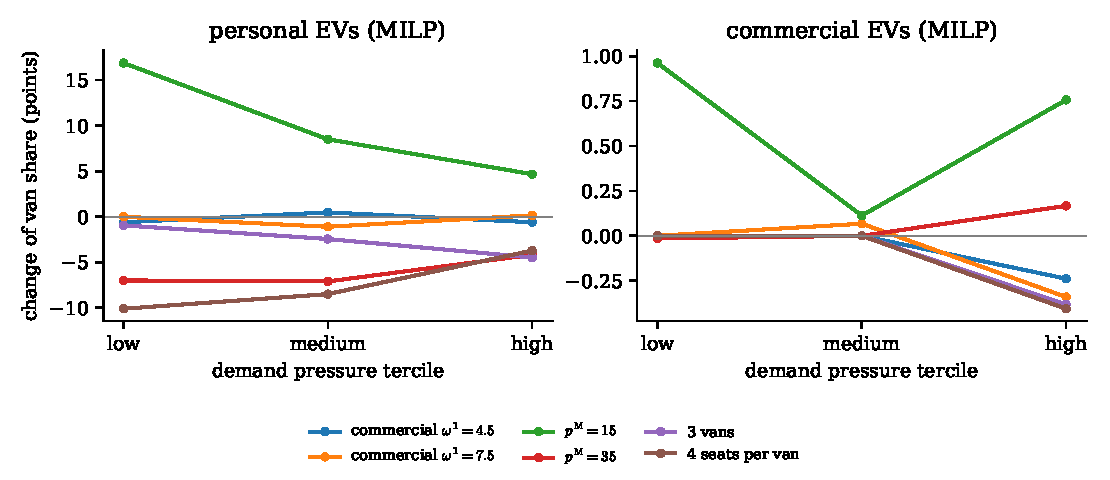
\includegraphics[width=0.92\textwidth]{figures/pressure_experiments.pdf}
\caption{Change of the van share at low, medium and high pressure for six variants (MILP).}\end{figure}
Formulation 4 predicts $\partial\Delta^{\mathrm C}_i/\partial q^{\mathrm F}_i=-(\omega+\delta)$: the larger $\omega$, the more a queued commercial EV gains from a van, so a higher $\omega^1$ should raise the commercial van share at high pressure and a lower one reduce it.
\begin{itemize}
  \item Across EVs the prediction holds in the baseline (commercial van users are at peak and queue-driven, Section~\ref{sec:peak}).
  \item Across variants it does not: at high pressure the commercial van share changes by \PredOmegaUpHigh{} points for $\omega^1=7.5$ and \PredOmegaDnHigh{} points for $\omega^1=4.5$ (MILP, baseline \PXEfiveComHiVanBCommercialHigh\pct); both are below the noise of time-limit plans and of opposite sign to the prediction for the increase. On the optimal pairs there is nothing to test: their high-pressure commercial EVs (\PredOptEfiveComHiN{}) neither queue nor use a van in either run.
  \item A likely reason: at the baseline $\omega$, the van premium ($p^{\mathrm M}-p^{\mathrm F}$ times $E$, weighted by the high $\mu$ of poor drivers) is far larger than $\pm25\pct$ of the downtime saved, so the threshold barely moves; queues push only the few commercial EVs with the longest waits.
\end{itemize}
\inshort{The private owners' value of charging time decides how many of them get vans; the commercial downtime rate changes what commercial drivers feel, not where they charge. The peak mechanism exists but is not sensitive to $\pm25\pct$ of $\omega$.}

%---------------------------------------------------------------------
\section{E6: money sensitivity at \texorpdfstring{$\theta=0$}{theta=0}}\label{sec:e6}
\begin{table}[H]\centering
\scriptsize
\caption{E6: every variant against its own baseline, for the three runs (paired instances; van shares and vans used: baseline $\to$ variant on the same paired instances).}\label{tab:expE6}
\begin{adjustbox}{max width=\textwidth}\begin{tabular}{llrrrrrrrrrr}\toprule
variant & method & valid & paired & \shortstack{newly valid\\/ lost} & \shortstack{mean\\$\Delta Z$ (\%)} & \shortstack{median\\$\Delta Z$ (\%)} & \shortstack{operator\\(\%)} & \shortstack{customers\\(\%)} & \shortstack{van share\\personal (\%)} & \shortstack{van share\\commercial (\%)} & vans used \\ \midrule
personal $\mu^{0}=1.125$ & MILP & 473 & 472 & +1/$-$2 & $-$1.35 & $-$1.29 & $-$0.01 & $-$1.96 & 19.9$\to$19.8 & 0.72$\to$0.61 & 2.18$\to$2.18 \\
 & RL zero-shot & 500 & 499 & +1/$-$1 & $-$1.28 & $-$1.23 & +0.10 & $-$1.89 & 6.7$\to$7.0 & 0.93$\to$0.86 & 2.20$\to$2.21 \\
 & RL retrained & 501 & 500 & +1/$-$0 & $-$1.22 & $-$1.19 & +0.07 & $-$1.79 & 6.7$\to$7.8 & 0.94$\to$0.73 & 2.21$\to$2.21 \\
personal $\mu^{0}=1.875$ & MILP & 475 & 473 & +2/$-$1 & +1.33 & +1.27 & $-$0.15 & +2.04 & 19.9$\to$18.9 & 0.72$\to$0.70 & 2.19$\to$2.18 \\
 & RL zero-shot & 500 & 499 & +1/$-$1 & +1.29 & +1.25 & $-$0.02 & +1.89 & 6.7$\to$6.5 & 0.93$\to$0.85 & 2.20$\to$2.21 \\
 & RL retrained & 499 & 499 & +0/$-$1 & +1.36 & +1.26 & +0.09 & +1.94 & 6.7$\to$7.3 & 0.91$\to$0.83 & 2.20$\to$2.22 \\
commercial $\mu^{0}=1.125$ & MILP & 475 & 474 & +1/$-$0 & $-$6.38 & $-$6.52 & +0.05 & $-$9.40 & 19.9$\to$19.6 & 0.73$\to$0.73 & 2.19$\to$2.20 \\
 & RL zero-shot & 499 & 499 & +0/$-$1 & $-$6.31 & $-$6.46 & +0.08 & $-$9.18 & 6.7$\to$6.8 & 0.91$\to$0.88 & 2.20$\to$2.21 \\
 & RL retrained & 500 & 500 & +0/$-$0 & $-$6.25 & $-$6.45 & $-$0.12 & $-$9.01 & 6.7$\to$7.1 & 0.94$\to$0.79 & 2.21$\to$2.19 \\
commercial $\mu^{0}=1.875$ & MILP & 475 & 473 & +2/$-$1 & +6.43 & +6.52 & +0.06 & +9.47 & 19.9$\to$19.8 & 0.72$\to$0.72 & 2.19$\to$2.19 \\
 & RL zero-shot & 500 & 499 & +1/$-$1 & +6.34 & +6.45 & +0.04 & +9.19 & 6.7$\to$6.8 & 0.93$\to$0.86 & 2.20$\to$2.21 \\
 & RL retrained & 500 & 499 & +1/$-$1 & +6.33 & +6.41 & +0.12 & +9.15 & 6.7$\to$7.8 & 0.91$\to$0.60 & 2.20$\to$2.21 \\
\bottomrule\end{tabular}\end{adjustbox}\end{table}

\begin{table}[H]\centering
\small
\caption{E6, MILP: van share of free-choice EVs (\%) by segment and income band, on the 472 instances valid in the baseline and every variant.}\label{tab:bandE6}
\begin{adjustbox}{max width=\textwidth}\begin{tabular}{lrrrrrr}\toprule
segment & income $\theta$ & baseline & personal $\mu^{0}=1.125$ & personal $\mu^{0}=1.875$ & commercial $\mu^{0}=1.125$ & commercial $\mu^{0}=1.875$ \\ \midrule
personal & 0.0--0.2 & 0.0 & 0.0 & 0.0 & 0.0 & 0.0 \\
 & 0.2--0.4 & 0.0 & 0.2 & 0.2 & 0.0 & 0.0 \\
 & 0.4--0.6 & 2.1 & 2.6 & 1.7 & 2.2 & 2.6 \\
 & 0.6--0.8 & 9.7 & 11.2 & 7.9 & 9.8 & 9.8 \\
 & 0.8--1.0 & 40.8 & 39.3 & 39.6 & 39.7 & 40.3 \\
commercial & 0.0--0.2 & 1.5 & 1.6 & 1.5 & 1.3 & 1.3 \\
 & 0.2--0.4 & 1.0 & 0.7 & 0.9 & 1.0 & 1.0 \\
 & 0.4--0.6 & 0.1 & 0.1 & 0.1 & 0.2 & 0.1 \\
 & 0.6--0.8 & 0.0 & 0.0 & 0.1 & 0.2 & 0.2 \\
 & 0.8--1.0 & 0.0 & 0.0 & 0.0 & 0.0 & 0.0 \\
\bottomrule\end{tabular}\end{adjustbox}\end{table}

\begin{figure}[H]\centering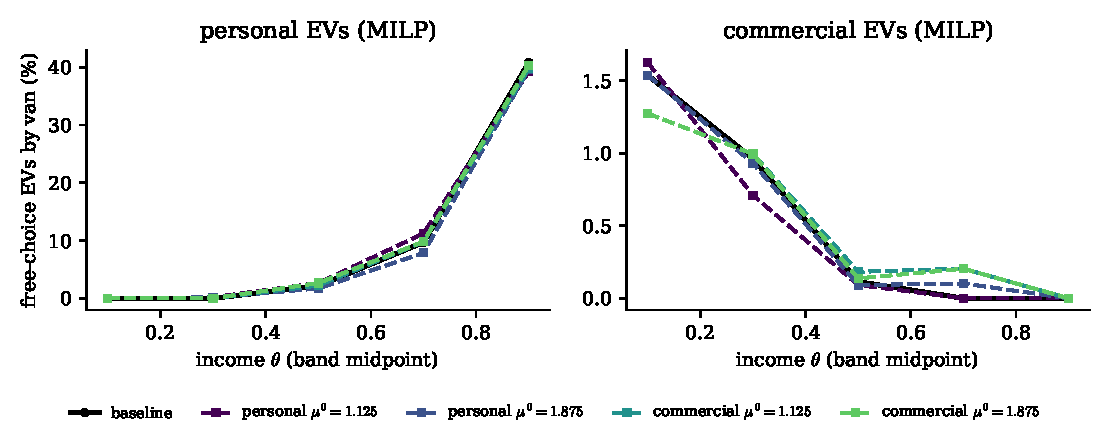
\includegraphics[width=0.92\textwidth]{figures/vanshare_E6.pdf}
\caption{E6, MILP: van share by income band, baseline and variants.}\end{figure}
\begin{table}[H]\centering
\scriptsize
\caption{E6, MILP: change of the perceived cost (\%) and of the money paid (Rs) per EV, by segment and income band (all EVs of the paired instances, stranded EVs included: they always pay the van tariff).}\label{tab:eqE6}
\begin{adjustbox}{max width=\textwidth}\begin{tabular}{llrrrrrrrr}\toprule
segment & income $\theta$ & \shortstack{personal $\mu^{0}=1.125$\\perceived (\%)} & \shortstack{paid\\(Rs)} & \shortstack{personal $\mu^{0}=1.875$\\perceived (\%)} & \shortstack{paid\\(Rs)} & \shortstack{commercial $\mu^{0}=1.125$\\perceived (\%)} & \shortstack{paid\\(Rs)} & \shortstack{commercial $\mu^{0}=1.875$\\perceived (\%)} & \shortstack{paid\\(Rs)} \\ \midrule
personal & 0.0--0.2 & $-$18.3 & $-$0 & +19.3 & $-$0 & +0.1 & $-$1 & +0.3 & $-$0 \\
 & 0.2--0.4 & $-$12.9 & +0 & +14.0 & +0 & +0.3 & +0 & +0.5 & +0 \\
 & 0.4--0.6 & $-$9.3 & +1 & +9.6 & $-$1 & +0.1 & +0 & $-$0.2 & +1 \\
 & 0.6--0.8 & $-$5.3 & +2 & +5.8 & $-$3 & +0.1 & +0 & +0.1 & $-$0 \\
 & 0.8--1.0 & $-$1.6 & $-$2 & +2.2 & $-$2 & +0.2 & $-$1 & +0.2 & $-$1 \\
commercial & 0.0--0.2 & $-$0.0 & $-$0 & $-$0.2 & $-$0 & $-$18.1 & $-$0 & +17.5 & $-$1 \\
 & 0.2--0.4 & $-$0.3 & $-$0 & $-$0.1 & +0 & $-$15.0 & +0 & +15.2 & +0 \\
 & 0.4--0.6 & $-$0.1 & $-$0 & +0.1 & +0 & $-$11.3 & +0 & +11.2 & $-$0 \\
 & 0.6--0.8 & +0.3 & +0 & +0.1 & +0 & $-$8.0 & +0 & +8.1 & +0 \\
 & 0.8--1.0 & +0.7 & +0 & $-$0.3 & $-$0 & $-$2.7 & +1 & +4.5 & +0 \\
\bottomrule\end{tabular}\end{adjustbox}\end{table}

\begin{itemize}
  \item \textbf{Commercial $\mu^0$ is the factor with the largest effect on $Z$}: \dZEsixComLoMilp\pct{} / \dZEsixComHiMilp\pct{} for $\pm25\pct$. The effect is almost all in the commercial perceived cost (\CcComEsixComLoMilp\pct{} / \CcComEsixComHiMilp\pct); the operator's cost does not move (\dOpEsixComLoMilp\pct{} / \dOpEsixComHiMilp\pct).
  \item Personal $\mu^0$ has a smaller effect (\dZEsixPersLoMilp\pct{} / \dZEsixPersHiMilp\pct), because private owners are fewer and richer.
  \item \textbf{Nobody changes resource}: the van shares stay within two points of the baseline in every band (Table~\ref{tab:bandE6}). The plan stays the same; only the rupee weights change. This is the envelope-theorem situation: the change of $Z$ equals the share of $Z$ carried by the coefficient.
  \item RL agrees almost exactly (\dZEsixComLoRt\pct{} / \dZEsixComHiRt\pct{} retrained).
\end{itemize}
\inshort{How strongly poor commercial drivers feel money is the most influential number of the model for $Z$, but it changes no decision.}

%---------------------------------------------------------------------
\section{E1: van tariff \texorpdfstring{$p^{\mathrm M}$}{pM}}\label{sec:e1}
\begin{table}[H]\centering
\scriptsize
\caption{E1: every variant against its own baseline, for the three runs (paired instances; van shares and vans used: baseline $\to$ variant on the same paired instances).}\label{tab:expE1}
\begin{adjustbox}{max width=\textwidth}\begin{tabular}{llrrrrrrrrrr}\toprule
variant & method & valid & paired & \shortstack{newly valid\\/ lost} & \shortstack{mean\\$\Delta Z$ (\%)} & \shortstack{median\\$\Delta Z$ (\%)} & \shortstack{operator\\(\%)} & \shortstack{customers\\(\%)} & \shortstack{van share\\personal (\%)} & \shortstack{van share\\commercial (\%)} & vans used \\ \midrule
$p^{\mathrm M}=15$ & MILP & 471 & 470 & +1/$-$4 & $-$4.19 & $-$4.14 & +3.69 & $-$7.80 & 19.8$\to$31.4 & 0.73$\to$1.38 & 2.17$\to$2.40 \\
 & RL zero-shot & 500 & 499 & +1/$-$1 & $-$3.74 & $-$3.56 & +0.45 & $-$5.66 & 6.7$\to$8.4 & 0.91$\to$1.02 & 2.20$\to$2.22 \\
 & RL retrained & 499 & 499 & +0/$-$1 & $-$3.78 & $-$3.61 & +1.04 & $-$5.97 & 6.7$\to$11.3 & 0.91$\to$1.03 & 2.20$\to$2.26 \\
$p^{\mathrm M}=35$ & MILP & 477 & 474 & +3/$-$0 & +3.91 & +3.88 & $-$1.39 & +6.53 & 19.9$\to$13.5 & 0.73$\to$0.76 & 2.19$\to$2.12 \\
 & RL zero-shot & 499 & 498 & +1/$-$2 & +3.64 & +3.52 & $-$0.36 & +5.49 & 6.7$\to$5.1 & 0.90$\to$0.75 & 2.20$\to$2.18 \\
 & RL retrained & 500 & 499 & +1/$-$1 & +3.73 & +3.57 & $-$0.76 & +5.80 & 6.7$\to$1.1 & 0.91$\to$0.92 & 2.20$\to$2.18 \\
\bottomrule\end{tabular}\end{adjustbox}\end{table}

\begin{figure}[H]\centering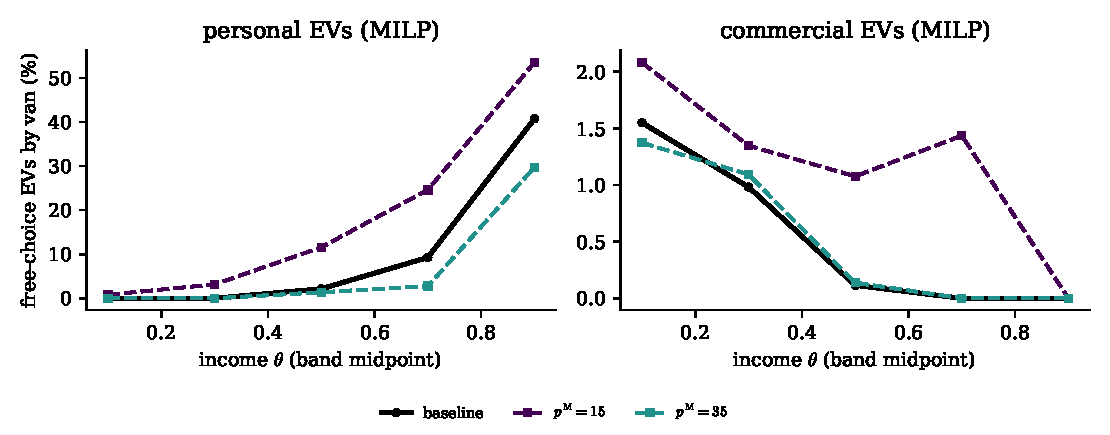
\includegraphics[width=0.92\textwidth]{figures/vanshare_E1.pdf}
\caption{E1, MILP: van share by income band, baseline and variants.}\end{figure}
\begin{table}[H]\centering
\small
\caption{E1, MILP: van share of free-choice EVs (\%) by segment and income band, on the 470 instances valid in the baseline and every variant.}\label{tab:bandE1}
\begin{adjustbox}{max width=\textwidth}\begin{tabular}{lrrrr}\toprule
segment & income $\theta$ & baseline & $p^{\mathrm M}=15$ & $p^{\mathrm M}=35$ \\ \midrule
personal & 0.0--0.2 & 0.0 & 0.8 & 0.0 \\
 & 0.2--0.4 & 0.0 & 3.2 & 0.0 \\
 & 0.4--0.6 & 2.1 & 11.6 & 1.4 \\
 & 0.6--0.8 & 9.3 & 24.6 & 2.8 \\
 & 0.8--1.0 & 40.7 & 53.5 & 29.7 \\
commercial & 0.0--0.2 & 1.6 & 2.1 & 1.4 \\
 & 0.2--0.4 & 1.0 & 1.3 & 1.1 \\
 & 0.4--0.6 & 0.1 & 1.1 & 0.1 \\
 & 0.6--0.8 & 0.0 & 1.4 & 0.0 \\
 & 0.8--1.0 & 0.0 & 0.0 & 0.0 \\
\bottomrule\end{tabular}\end{adjustbox}\end{table}

\begin{table}[H]\centering
\scriptsize
\caption{E1, MILP: change of the perceived cost (\%) and of the money paid (Rs) per EV, by segment and income band (all EVs of the paired instances, stranded EVs included: they always pay the van tariff).}\label{tab:eqE1}
\begin{adjustbox}{max width=\textwidth}\begin{tabular}{llrrrr}\toprule
segment & income $\theta$ & \shortstack{$p^{\mathrm M}=15$\\perceived (\%)} & \shortstack{paid\\(Rs)} & \shortstack{$p^{\mathrm M}=35$\\perceived (\%)} & \shortstack{paid\\(Rs)} \\ \midrule
personal & 0.0--0.2 & +0.1 & $-$0 & +1.7 & +0 \\
 & 0.2--0.4 & $-$5.6 & $-$30 & +5.5 & +30 \\
 & 0.4--0.6 & $-$7.8 & $-$36 & +5.4 & +32 \\
 & 0.6--0.8 & $-$10.6 & $-$39 & +4.5 & +17 \\
 & 0.8--1.0 & $-$15.4 & $-$88 & +10.1 & +49 \\
commercial & 0.0--0.2 & $-$5.0 & $-$21 & +4.5 & +20 \\
 & 0.2--0.4 & $-$6.9 & $-$35 & +7.0 & +35 \\
 & 0.4--0.6 & $-$5.8 & $-$31 & +5.7 & +31 \\
 & 0.6--0.8 & $-$5.9 & $-$39 & +6.5 & +40 \\
 & 0.8--1.0 & $-$0.1 & $-$0 & +0.7 & +1 \\
\bottomrule\end{tabular}\end{adjustbox}\end{table}

\begin{itemize}
  \item \textbf{Who gets vans.} Without a premium ($p^{\mathrm M}=15$) the van share of private owners rises from \VanPBEonePMLoMilp\pct{} to \VanPEonePMLoMilp\pct{} (top band \VanPersTopBEonePMLo\pct{} $\to$ \VanPersTopEonePMLo\pct) and reaches the middle bands; commercial drivers move little (\VanCBEonePMLoMilp\pct{} $\to$ \VanCEonePMLoMilp\pct). At $p^{\mathrm M}=35$ the private share falls to \VanPEonePMHiMilp\pct.
  \item \textbf{At what cost.} $p^{\mathrm M}=15$: $Z$ \dZEonePMLoMilp\pct, the customers \dCuEonePMLoMilp\pct, the operator \dOpEonePMLoMilp\pct{} (more vans: \VansBEonePMLoMilp{} $\to$ \VansEonePMLoMilp{} per instance). $p^{\mathrm M}=35$: $Z$ \dZEonePMHiMilp\pct, the operator \dOpEonePMHiMilp\pct.
  \item \textbf{Equity} (Table~\ref{tab:eqE1}, all EVs including the stranded, who must take the van). The richest private owners gain most from cheaper vans (perceived cost \CcPersTopEonePMLo\pct) and lose most from dearer ones (\CcPersTopEonePMHi\pct). Commercial drivers gain or lose a similar share in every band below the top (poorest band \CcComLowEonePMLo\pct{} / \CcComLowEonePMHi\pct): almost all of it is paid by \emph{stranded} commercial EVs, who have no station in range and pay the van tariff whatever it is. The tariff is therefore also a charge on the customers with no choice.
  \item \textbf{Peak and off-peak} (Table~\ref{tab:pressexp}): the extra van seats of $p^{\mathrm M}=15$ go mostly to private owners at low pressure (\PXEonePMLoVanPersonalLow{} points, against \PXEonePMLoVanPersonalHigh{} at high pressure); at peak the seats are already taken.
  \item RL measures the same change of $Z$ (\dZEonePMLoRt\pct{} / \dZEonePMHiRt\pct) and the same direction of the private van share (\VanPBEonePMLoRt\pct{} $\to$ \VanPEonePMLoRt\pct{} retrained, \VanPEonePMLoZs\pct{} zero-shot): retraining makes RL's response much stronger.
\end{itemize}
\inshort{The van tariff is the operator's lever on who gets vans: removing the premium helps rich private owners most, costs the operator more and lowers the total cost; for commercial drivers it acts mainly through the stranded EVs, who pay it without choice.}

\clearpage
\section{E2: van fleet and seats}\label{sec:e2}
\begin{table}[H]\centering
\scriptsize
\caption{E2: every variant against its own baseline, for the three runs (paired instances; van shares and vans used: baseline $\to$ variant on the same paired instances).}\label{tab:expE2}
\begin{adjustbox}{max width=\textwidth}\begin{tabular}{llrrrrrrrrrr}\toprule
variant & method & valid & paired & \shortstack{newly valid\\/ lost} & \shortstack{mean\\$\Delta Z$ (\%)} & \shortstack{median\\$\Delta Z$ (\%)} & \shortstack{operator\\(\%)} & \shortstack{customers\\(\%)} & \shortstack{van share\\personal (\%)} & \shortstack{van share\\commercial (\%)} & vans used \\ \midrule
3 vans & MILP & 441 & 441 & +0/$-$33 & $-$0.04 & +0.00 & $-$0.53 & +0.19 & 19.4$\to$17.4 & 0.17$\to$0.11 & 2.02$\to$1.96 \\
 & RL zero-shot & 465 & 465 & +0/$-$35 & +0.02 & +0.00 & $-$0.27 & +0.15 & 6.4$\to$5.7 & 0.31$\to$0.23 & 2.03$\to$2.00 \\
 & RL retrained & 466 & 466 & +0/$-$34 & +0.09 & +0.00 & $-$0.12 & +0.18 & 6.4$\to$5.9 & 0.39$\to$0.23 & 2.03$\to$2.02 \\
7 vans & MILP & 487 & 474 & +13/$-$0 & +0.02 & +0.00 & +0.22 & $-$0.05 & 19.9$\to$20.5 & 0.73$\to$0.71 & 2.19$\to$2.22 \\
 & RL zero-shot & 506 & 500 & +6/$-$0 & +0.04 & +0.00 & +0.13 & +0.02 & 6.7$\to$6.7 & 0.94$\to$1.01 & 2.21$\to$2.23 \\
 & RL retrained & 506 & 500 & +6/$-$0 & +0.00 & +0.00 & +0.06 & $-$0.00 & 6.7$\to$7.0 & 0.94$\to$0.68 & 2.21$\to$2.23 \\
4 seats per van & MILP & 471 & 467 & +4/$-$7 & +1.08 & +0.80 & +3.03 & +0.26 & 19.8$\to$11.6 & 0.33$\to$0.25 & 2.15$\to$2.48 \\
 & RL zero-shot & 493 & 493 & +0/$-$7 & +0.91 & +0.19 & +3.87 & $-$0.35 & 6.7$\to$5.8 & 0.46$\to$0.37 & 2.17$\to$2.54 \\
 & RL retrained & 494 & 494 & +0/$-$6 & +0.88 & +0.34 & +4.04 & $-$0.46 & 6.8$\to$7.3 & 0.52$\to$0.33 & 2.18$\to$2.55 \\
8 seats per van & MILP & 471 & 471 & +0/$-$3 & $-$0.08 & +0.00 & $-$0.28 & +0.06 & 19.8$\to$21.6 & 0.73$\to$0.82 & 2.18$\to$2.13 \\
 & RL zero-shot & 500 & 499 & +1/$-$1 & $-$0.08 & +0.00 & $-$0.61 & +0.16 & 6.7$\to$6.6 & 0.93$\to$0.92 & 2.20$\to$2.13 \\
 & RL retrained & 499 & 499 & +0/$-$1 & +0.07 & +0.01 & $-$0.31 & +0.25 & 6.7$\to$7.2 & 0.91$\to$0.94 & 2.20$\to$2.16 \\
\bottomrule\end{tabular}\end{adjustbox}\end{table}

\begin{table}[H]\centering
\small
\caption{E2, MILP: mean $\Delta Z$ (\%) by family on paired instances; in brackets the instances newly valid / no longer valid.}\label{tab:e2fam}
\begin{adjustbox}{max width=\textwidth}\begin{tabular}{lrrrrrr}\toprule
variant & C1 & C2 & R1 & R2 & RC1 & RC2 \\ \midrule
3 vans & +0.03 (0/2) & $-$0.09 (0/3) & +0.05 (0/11) & $-$0.04 (0/4) & $-$0.22 (0/12) & $-$0.08 (0/1) \\
7 vans & $-$0.02 (1/0) & +0.06 (1/0) & $-$0.03 (6/0) & +0.07 (0/0) & $-$0.09 (4/0) & +0.06 (1/0) \\
4 seats per van & +1.90 (0/1) & +1.06 (0/1) & $-$0.16 (2/0) & +2.11 (0/4) & +0.12 (2/1) & +0.50 (0/0) \\
8 seats per van & $-$0.16 (0/0) & $-$0.05 (0/0) & +0.03 (0/1) & $-$0.23 (0/0) & $-$0.04 (0/2) & +0.06 (0/0) \\
\bottomrule\end{tabular}\end{adjustbox}\end{table}

\begin{table}[H]\centering
\small
\caption{E2, MILP: van share of free-choice EVs (\%) by segment and income band, on the 441 instances valid in the baseline and every variant.}\label{tab:bandE2}
\begin{adjustbox}{max width=\textwidth}\begin{tabular}{lrrrrrr}\toprule
segment & income $\theta$ & baseline & 3 vans & 7 vans & 4 seats per van & 8 seats per van \\ \midrule
personal & 0.0--0.2 & 0.0 & 0.0 & 0.0 & 0.0 & 0.0 \\
 & 0.2--0.4 & 0.0 & 0.0 & 0.0 & 0.2 & 0.0 \\
 & 0.4--0.6 & 1.3 & 0.9 & 1.2 & 0.5 & 1.4 \\
 & 0.6--0.8 & 8.2 & 7.6 & 9.0 & 4.3 & 10.0 \\
 & 0.8--1.0 & 40.4 & 36.1 & 40.8 & 22.7 & 43.8 \\
commercial & 0.0--0.2 & 0.6 & 0.3 & 0.6 & 0.5 & 0.7 \\
 & 0.2--0.4 & 0.2 & 0.1 & 0.2 & 0.1 & 0.2 \\
 & 0.4--0.6 & 0.0 & 0.0 & 0.0 & 0.0 & 0.1 \\
 & 0.6--0.8 & 0.0 & 0.0 & 0.0 & 0.0 & 0.1 \\
 & 0.8--1.0 & 0.0 & 0.0 & 0.0 & 0.0 & 0.0 \\
\bottomrule\end{tabular}\end{adjustbox}\end{table}

\begin{table}[H]\centering
\small
\caption{Which van resource is closest to its limit (every dispatched van of the valid MILP plans; tightest = largest used share of seats, battery and time $T$).}\label{tab:vanlim}
\begin{adjustbox}{max width=\textwidth}\begin{tabular}{lrrrrrrrr}\toprule
run (MILP) & vans & \shortstack{full\\(\%)} & \shortstack{battery\\$>$90\,\% (\%)} & \shortstack{mean kWh\\drawn} & \shortstack{max kWh\\drawn} & \shortstack{tightest:\\seats (\%)} & \shortstack{tightest:\\battery (\%)} & \shortstack{tightest:\\time (\%)} \\ \midrule
baseline (5 vans, 6 seats, 150 kWh) & 1040 & 48.1 & 22.2 & 106.6 & 149.7 & 60.4 & 10.1 & 29.5 \\
3 vans & 866 & 55.1 & 26.4 & 109.7 & 149.9 & 66.5 & 10.2 & 23.3 \\
7 vans & 1052 & 47.2 & 22.4 & 106.2 & 150.0 & 59.1 & 10.2 & 30.7 \\
4 seats & 1159 & 75.5 & 0.0 & 83.9 & 133.4 & 80.1 & 0.0 & 19.9 \\
8 seats & 1005 & 4.9 & 37.6 & 111.0 & 150.0 & 8.1 & 59.4 & 32.5 \\
battery 200 kWh & 1011 & 52.4 & 0.1 & 108.1 & 180.8 & 69.8 & 0.0 & 30.2 \\
\bottomrule\end{tabular}\end{adjustbox}\end{table}

\begin{figure}[H]\centering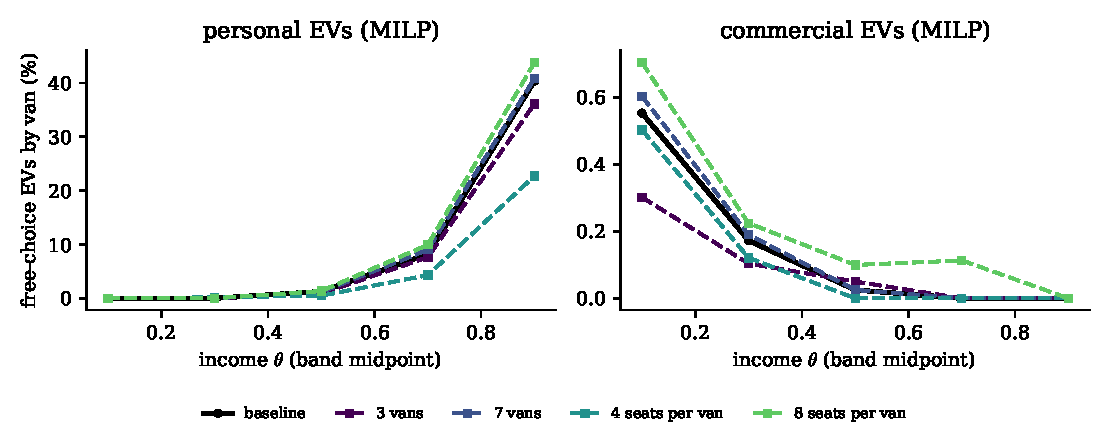
\includegraphics[width=0.92\textwidth]{figures/vanshare_E2.pdf}
\caption{E2, MILP: van share by income band, baseline and variants.}\end{figure}
\begin{itemize}
  \item \textbf{Vans decide feasibility, not cost.} With 3 vans \LostEtwoVansLoMilp{} instances lose their plan, with 7 vans \NewEtwoVansHiMilp{} gain one; most are in the short-horizon families R1 and RC1 (Table~\ref{tab:e2fam}), where vans run out of time. Where a plan exists, $Z$ hardly moves (\dZEtwoVansLoMilp\pct{} / \dZEtwoVansHiMilp\pct), and every optimal pair is unchanged.
  \item \textbf{Seats decide cost.} 4 seats per van raise $Z$ by \dZEtwoSeatsLoMilp\pct{}, all of it the operator's (\dOpEtwoSeatsLoMilp\pct): more vans leave (\VansBEtwoSeatsLoMilp{} $\to$ \VansEtwoSeatsLoMilp) and the seats of each are almost all taken (\SeatsBEtwoSeatsLoMilp\pct{} $\to$ \SeatsEtwoSeatsLoMilp\pct). The private van share falls to \VanPEtwoSeatsLoMilp\pct, most of it at low pressure (\PXEtwoSeatsLoVanPersonalLow{} points).
  \item \textbf{8 seats are idle}: $Z$ \dZEtwoSeatsHiMilp\pct, seats used \SeatsBEtwoSeatsHiMilp\pct{} $\to$ \SeatsEtwoSeatsHiMilp\pct. With 8 seats the battery becomes the tightest resource of most vans (Table~\ref{tab:vanlim}).
  \item \textbf{At peak}, fewer vans cost the private owners their seats (Table~\ref{tab:pressexp}: 3 vans, high pressure); commercial drivers lose little because they have few seats to lose.
  \item RL reproduces the losses of feasibility (\LostEtwoVansLoRt{} instances lost with 3 vans, \NewEtwoVansHiRt{} gained with 7) and the cost of 4 seats (\dZEtwoSeatsLoRt\pct), but not the drop of the private van share with 4 seats.
\end{itemize}
\inshort{Another van pays off only where it makes an instance feasible (R1, RC1); another seat pays off everywhere vans fill up; beyond 6 seats the extra seats are idle.}

%---------------------------------------------------------------------
\section{E8: van battery}\label{sec:e8}
\begin{table}[H]\centering
\scriptsize
\caption{E8: every variant against its own baseline, for the three runs (paired instances; van shares and vans used: baseline $\to$ variant on the same paired instances).}\label{tab:expE8}
\begin{adjustbox}{max width=\textwidth}\begin{tabular}{llrrrrrrrrrr}\toprule
variant & method & valid & paired & \shortstack{newly valid\\/ lost} & \shortstack{mean\\$\Delta Z$ (\%)} & \shortstack{median\\$\Delta Z$ (\%)} & \shortstack{operator\\(\%)} & \shortstack{customers\\(\%)} & \shortstack{van share\\personal (\%)} & \shortstack{van share\\commercial (\%)} & vans used \\ \midrule
battery 200 kWh & MILP & 476 & 473 & +3/$-$1 & $-$0.01 & +0.00 & $-$0.40 & +0.19 & 19.9$\to$18.5 & 0.72$\to$0.70 & 2.19$\to$2.14 \\
 & RL zero-shot & 501 & 500 & +1/$-$0 & $-$0.02 & +0.00 & $-$0.17 & +0.05 & 6.7$\to$6.5 & 0.94$\to$0.89 & 2.21$\to$2.19 \\
 & RL retrained & 500 & 499 & +1/$-$1 & $-$0.07 & +0.00 & $-$0.06 & $-$0.07 & 6.7$\to$8.2 & 0.91$\to$0.65 & 2.20$\to$2.18 \\
\bottomrule\end{tabular}\end{adjustbox}\end{table}

\begin{itemize}
  \item With 200\,kWh $Z$ changes by \dZEeightBatHiMilp\pct{} on average (\dZEeightBatHiRt\pct{} for \Rt), \EeightDecision{} the decision threshold of 1\pct{}. Of the \DirNEeightBatHi{} optimal pairs, \EeightOptChanged{} change at all.
  \item In the baseline \VanBninetyBase\pct{} of vans draw more than 90\pct{} of their battery, but the battery is the tightest resource for only \VanBattTightBase\pct{} of them (seats \VanSeatTightBase\pct, time \VanTimeTightBase\pct). With 200\,kWh it is tightest for \VanBattTightEeight\pct.
  \item \textbf{Decision: van recharging need not be modelled} at 6 seats. If the seats were raised to 8, the battery would become the main limit (Table~\ref{tab:vanlim}) and the question would have to be asked again.
\end{itemize}
\inshort{A larger battery changes nothing that matters: drop recharging, unless the seats per van grow.}

%=====================================================================
\section{E9: station capacity (RL only)}\label{sec:e9}
No MILP run exists for E9: the numbers are those of the retrained RL model against the baseline RL run, without a gap to the MILP or a direction check. Utilisation uses the variant's guns and power.
\begin{table}[H]\centering
\scriptsize
\caption{E9 (RL only): every variant against the baseline RL run (paired instances; van shares, vans used and the mean station queue of commercial EVs: baseline $\to$ variant).}\label{tab:expE9}
\begin{adjustbox}{max width=\textwidth}\begin{tabular}{llrrrrrrrrrrr}\toprule
variant & run & valid & paired & \shortstack{newly valid\\/ lost} & \shortstack{mean\\$\Delta Z$ (\%)} & \shortstack{median\\$\Delta Z$ (\%)} & \shortstack{operator\\(\%)} & \shortstack{customers\\(\%)} & \shortstack{van share\\personal (\%)} & \shortstack{van share\\commercial (\%)} & vans used & \shortstack{queue\\commercial (min)} \\ \midrule
1 gun per station & RL retrained & 432 & 432 & +0/$-$68 & +4.76 & +2.22 & +5.40 & +4.56 & 6.2$\to$16.7 & 0.04$\to$1.83 & 1.92$\to$2.29 & 1.18$\to$3.48 \\
4 guns per station & RL retrained & 509 & 500 & +9/$-$0 & $-$2.21 & $-$0.57 & $-$0.90 & $-$2.72 & 6.7$\to$5.3 & 0.94$\to$0.01 & 2.21$\to$2.13 & 2.50$\to$0.53 \\
11 kW per gun & RL retrained & 398 & 398 & +0/$-$102 & +20.13 & +19.04 & +25.61 & +18.42 & 6.3$\to$58.7 & 0.15$\to$2.27 & 1.93$\to$3.25 & 1.25$\to$0.77 \\
44 kW per gun & RL retrained & 532 & 500 & +32/$-$0 & $-$12.30 & $-$11.79 & $-$1.54 & $-$16.97 & 6.7$\to$0.0 & 0.94$\to$0.01 & 2.21$\to$2.12 & 2.50$\to$2.32 \\
\bottomrule\end{tabular}\end{adjustbox}\end{table}

\begin{table}[H]\centering
\small
\caption{E9, retrained RL: van share of free-choice EVs (\%) by segment and income band, on the 393 instances valid in the baseline and every variant.}\label{tab:bandE9}
\begin{adjustbox}{max width=\textwidth}\begin{tabular}{lrrrrrr}\toprule
segment & income $\theta$ & baseline RL & 1 gun per station & 4 guns per station & 11 kW per gun & 44 kW per gun \\ \midrule
personal & 0.0--0.2 & 0.0 & 0.0 & 0.0 & 5.4 & 0.0 \\
 & 0.2--0.4 & 0.0 & 2.2 & 0.0 & 5.7 & 0.0 \\
 & 0.4--0.6 & 0.0 & 4.7 & 0.0 & 29.4 & 0.0 \\
 & 0.6--0.8 & 4.6 & 14.3 & 4.1 & 58.9 & 0.0 \\
 & 0.8--1.0 & 12.1 & 27.0 & 10.6 & 88.1 & 0.0 \\
commercial & 0.0--0.2 & 0.0 & 1.4 & 0.0 & 2.6 & 0.0 \\
 & 0.2--0.4 & 0.1 & 2.4 & 0.0 & 1.9 & 0.0 \\
 & 0.4--0.6 & 0.0 & 1.2 & 0.0 & 1.8 & 0.0 \\
 & 0.6--0.8 & 0.0 & 0.8 & 0.0 & 1.5 & 0.0 \\
 & 0.8--1.0 & 0.0 & 0.0 & 0.0 & 1.3 & 0.0 \\
\bottomrule\end{tabular}\end{adjustbox}\end{table}

\begin{itemize}
  \item \textbf{Guns per station.} Halving the guns (12 instead of 24) raises $Z$ by \dZEnineGunsLoRt\pct{} (median \dZmedEnineGunsLoRt\pct; operator \dOpEnineGunsLoRt\pct, customers \dCuEnineGunsLoRt\pct) and makes \LostEnineGunsLoRt{} instances infeasible for RL, mostly R1 (\LostFamEnineGunsLoRone) and RC1 (\LostFamEnineGunsLoRCone). The commercial station queue grows from \QComBEnineGunsLoRt{} to \QComEnineGunsLoRt{} min and vans take over: private cars \VanPBEnineGunsLoRt\pct{} $\to$ \VanPEnineGunsLoRt\pct, commercial \VanCBEnineGunsLoRt\pct{} $\to$ \VanCEnineGunsLoRt\pct. Doubling the guns changes $Z$ by \dZEnineGunsHiRt\pct, makes \NewEnineGunsHiRt{} instances feasible and almost removes queues (\QComBEnineGunsHiRt{} $\to$ \QComEnineGunsHiRt{} min).
  \item \textbf{Power per gun.} 11\,kW doubles every station session: $Z$ \dZEninePowLoRt\pct{} (operator \dOpEninePowLoRt\pct), \LostEninePowLoRt{} instances lost, and vans become the main resource for private owners (\VanPBEninePowLoRt\pct{} $\to$ \VanPEninePowLoRt\pct; vans used \VansBEninePowLoRt{} $\to$ \VansEninePowLoRt). 44\,kW changes $Z$ by \dZEninePowHiRt\pct, almost all of it the customers' charging time (\dCuEninePowHiRt\pct), gains \NewEninePowHiRt{} instances, and private van use falls to \VanPEninePowHiRt\pct.
  \item \textbf{Peak} (Table~\ref{tab:pressrl}): with 1 gun per station the extra van use is at high pressure (private \PXEnineGunsLoVanPersonalHigh, commercial \PXEnineGunsLoVanCommercialHigh{} points), where the commercial queue grows from \PXEnineGunsLoQBHigh{} to \PXEnineGunsLoQHigh{} min: the queue-driven switch of commercial EVs to vans that E5 could not show appears clearly once station capacity is cut.
  \item \textbf{Utilisation} (Table~\ref{tab:utilrl}): with 12 guns a gun is busy \UXEnineGunsLoGunRt\pct{} of the period (baseline \UXBEnineGunsLoGunRt\pct); with 11\,kW \UXEninePowLoGunRt\pct, and the vans carry \UXEninePowLoVanEnergyRt\pct{} of the energy (baseline \UXBEninePowLoVanEnergyRt\pct). With 48 guns \UXEnineGunsHiIdleGunsRt{} guns per instance stay idle.
\end{itemize}
\inshort{Station power matters far more than the number of guns: halving the power raises the cost by a fifth and moves private owners to vans; halving the guns costs a few per cent but creates peak queues that push commercial drivers to vans. Cutting either loses many short-horizon instances.}

\section{E10: charging demand (RL only)}\label{sec:e10}
No MILP run exists for E10. Energy per EV is scaled by 0.75 or 1.25; this changes every charging time, so the pressure window changes too, but the baseline labels are kept.
\begin{table}[H]\centering
\scriptsize
\caption{E10 (RL only): every variant against the baseline RL run (paired instances; van shares, vans used and the mean station queue of commercial EVs: baseline $\to$ variant).}\label{tab:expE10}
\begin{adjustbox}{max width=\textwidth}\begin{tabular}{llrrrrrrrrrrr}\toprule
variant & run & valid & paired & \shortstack{newly valid\\/ lost} & \shortstack{mean\\$\Delta Z$ (\%)} & \shortstack{median\\$\Delta Z$ (\%)} & \shortstack{operator\\(\%)} & \shortstack{customers\\(\%)} & \shortstack{van share\\personal (\%)} & \shortstack{van share\\commercial (\%)} & vans used & \shortstack{queue\\commercial (min)} \\ \midrule
energy per EV $\times0.75$ & RL retrained & 539 & 500 & +39/$-$0 & $-$21.82 & $-$21.79 & $-$18.59 & $-$23.35 & 6.7$\to$6.1 & 0.94$\to$0.12 & 2.21$\to$2.00 & 2.50$\to$2.48 \\
energy per EV $\times1.25$ & RL retrained & 421 & 421 & +0/$-$79 & +22.19 & +21.96 & +19.33 & +23.57 & 6.3$\to$5.5 & 0.40$\to$0.77 & 1.99$\to$2.19 & 1.60$\to$1.57 \\
\bottomrule\end{tabular}\end{adjustbox}\end{table}

\begin{table}[H]\centering
\small
\caption{E10, retrained RL: van share of free-choice EVs (\%) by segment and income band, on the 421 instances valid in the baseline and every variant.}\label{tab:bandE10}
\begin{adjustbox}{max width=\textwidth}\begin{tabular}{lrrrr}\toprule
segment & income $\theta$ & baseline RL & energy per EV $\times0.75$ & energy per EV $\times1.25$ \\ \midrule
personal & 0.0--0.2 & 0.0 & 0.0 & 0.0 \\
 & 0.2--0.4 & 0.0 & 0.0 & 0.6 \\
 & 0.4--0.6 & 0.0 & 0.2 & 0.8 \\
 & 0.6--0.8 & 4.6 & 5.2 & 3.7 \\
 & 0.8--1.0 & 12.0 & 11.6 & 10.1 \\
commercial & 0.0--0.2 & 0.2 & 0.0 & 0.5 \\
 & 0.2--0.4 & 0.5 & 0.0 & 0.9 \\
 & 0.4--0.6 & 0.4 & 0.0 & 0.8 \\
 & 0.6--0.8 & 0.1 & 0.1 & 0.6 \\
 & 0.8--1.0 & 0.0 & 0.0 & 0.0 \\
\bottomrule\end{tabular}\end{adjustbox}\end{table}

\begin{table}[H]\centering
\small
\caption{E9 and E10, retrained RL: mean $\Delta Z$ (\%) by family on paired instances; in brackets the instances newly valid / no longer valid.}\label{tab:rlfam}
\begin{adjustbox}{max width=\textwidth}\begin{tabular}{lrrrrrr}\toprule
variant & C1 & C2 & R1 & R2 & RC1 & RC2 \\ \midrule
1 gun per station & +3.16 (0/4) & +3.62 (0/4) & +6.44 (0/28) & +4.29 (0/7) & +11.48 (0/22) & +4.35 (0/3) \\
4 guns per station & $-$1.34 (0/0) & $-$1.59 (1/0) & $-$2.97 (2/0) & $-$1.67 (0/0) & $-$5.88 (6/0) & $-$1.33 (0/0) \\
11 kW per gun & +19.71 (0/3) & +18.64 (0/3) & +24.89 (0/45) & +18.90 (0/4) & +47.83 (0/44) & +18.15 (0/3) \\
44 kW per gun & $-$12.39 (0/0) & $-$13.39 (1/0) & $-$12.21 (4/0) & $-$11.35 (0/0) & $-$15.97 (27/0) & $-$10.13 (0/0) \\
energy per EV $\times0.75$ & $-$22.05 (0/0) & $-$21.96 (1/0) & $-$21.94 (10/0) & $-$21.13 (0/0) & $-$22.54 (28/0) & $-$21.75 (0/0) \\
energy per EV $\times1.25$ & +22.22 (0/2) & +22.05 (0/1) & +23.32 (0/34) & +21.51 (0/2) & +25.13 (0/39) & +21.95 (0/1) \\
\bottomrule\end{tabular}\end{adjustbox}\end{table}

\begin{table}[H]\centering
\scriptsize
\caption{E9 and E10, retrained RL, at low and high demand pressure (baseline pressure labels): change of the van share of free-choice EVs (points) and mean station queue of commercial station users, baseline $\to$ variant.}\label{tab:pressrl}
\begin{adjustbox}{max width=\textwidth}\begin{tabular}{lrrcrrc}\toprule
variant & \shortstack{low: van\\personal} & \shortstack{low: van\\commercial} & \shortstack{low: queue\\commercial (min)} & \shortstack{high: van\\personal} & \shortstack{high: van\\commercial} & \shortstack{high: queue\\commercial (min)} \\ \midrule
1 gun per station & +5.8 & +0.0 & 0.15$\to$0.63 & +29.5 & +11.6 & 8.12$\to$14.53 \\
4 guns per station & $-$0.6 & $-$0.0 & 0.18$\to$0.02 & $-$3.0 & $-$3.6 & 11.76$\to$2.65 \\
11 kW per gun & +55.0 & +1.1 & 0.14$\to$0.44 & +46.5 & +9.1 & 9.31$\to$4.15 \\
44 kW per gun & $-$9.4 & $-$0.0 & 0.18$\to$0.13 & $-$4.4 & $-$3.6 & 11.76$\to$9.72 \\
energy per EV $\times0.75$ & $-$0.1 & $-$0.0 & 0.18$\to$0.13 & $-$1.4 & $-$3.2 & 11.76$\to$11.11 \\
energy per EV $\times1.25$ & $-$2.4 & $-$0.0 & 0.14$\to$0.27 & +3.7 & +2.1 & 10.31$\to$9.09 \\
\bottomrule\end{tabular}\end{adjustbox}\end{table}

\begin{table}[H]\centering
\scriptsize
\caption{E9 and E10: utilisation, baseline RL $\to$ variant, with the variant's capacities (guns per station, kW per gun, energy per EV); means of per-instance and per-van shares, paired instances.}\label{tab:utilrl}
\begin{adjustbox}{max width=\textwidth}\begin{tabular}{llccccccc}\toprule
variant & run & \shortstack{gun\\util. (\%)} & \shortstack{idle guns\\per inst.} & \shortstack{van share\\of kWh (\%)} & \shortstack{fleet\\use (\%)} & \shortstack{seats\\(\%)} & \shortstack{battery\\(\%)} & \shortstack{installed\\capacity (\%)} \\ \midrule
1 gun per station & RL retrained & 11.2$\to$21.0 & 6.7$\to$2.0 & 16.7$\to$19.9 & 38$\to$46 & 71$\to$72 & 64$\to$68 & 10.4$\to$17.0 \\
4 guns per station & RL retrained & 15.8$\to$8.0 & 5.8$\to$18.5 & 16.9$\to$16.3 & 44$\to$43 & 68$\to$67 & 62$\to$61 & 14.7$\to$8.3 \\
11 kW per gun & RL retrained & 9.3$\to$15.5 & 6.8$\to$7.4 & 17.1$\to$31.7 & 39$\to$65 & 74$\to$80 & 67$\to$76 & 8.8$\to$14.4 \\
44 kW per gun & RL retrained & 15.8$\to$8.1 & 5.8$\to$6.8 & 16.9$\to$14.5 & 44$\to$42 & 68$\to$61 & 62$\to$56 & 14.7$\to$8.3 \\
energy per EV $\times0.75$ & RL retrained & 15.8$\to$12.0 & 5.8$\to$6.3 & 16.9$\to$16.6 & 44$\to$40 & 68$\to$72 & 62$\to$51 & 14.7$\to$11.0 \\
energy per EV $\times1.25$ & RL retrained & 10.6$\to$13.2 & 6.4$\to$6.9 & 17.2$\to$16.9 & 40$\to$44 & 73$\to$66 & 66$\to$74 & 9.9$\to$12.4 \\
\bottomrule\end{tabular}\end{adjustbox}\end{table}

\begin{itemize}
  \item \textbf{$Z$ moves almost in proportion to the energy}: \dZEtenDemLoRt\pct{} at $\times0.75$ and \dZEtenDemHiRt\pct{} at $\times1.25$ (elasticity \ElastEnergyRl), operator and customers alike (\dOpEtenDemHiRt\pct{} / \dCuEtenDemHiRt\pct{} at $\times1.25$): energy, tariffs and charging time all scale with $E$.
  \item \textbf{Feasibility}: $\times1.25$ loses \LostEtenDemHiRt{} instances (R1 \LostFamEtenDemHiRone, RC1 \LostFamEtenDemHiRCone): in the 230--240-minute horizons the longer sessions no longer fit. $\times0.75$ makes \NewEtenDemLoRt{} instances feasible.
  \item \textbf{Who gets vans} changes little: private van share \VanPBEtenDemHiRt\pct{} $\to$ \VanPEtenDemHiRt\pct{} at $\times1.25$; vans used \VansBEtenDemHiRt{} $\to$ \VansEtenDemHiRt.
  \item \textbf{Utilisation}: at $\times1.25$ a gun is busy \UXEtenDemHiGunRt\pct{} of the period (baseline \UXBEtenDemHiGunRt\pct) and the installed capacity is used at \UXEtenDemHiSystemRt\pct{} (baseline \UXBEtenDemHiSystemRt\pct).
\end{itemize}
\inshort{Energy per EV scales the whole problem: the cost moves almost one for one, the short horizons lose feasibility, but the allocation between stations and vans hardly changes.}

\section{All experiments side by side}\label{sec:synth}
\begin{figure}[H]\centering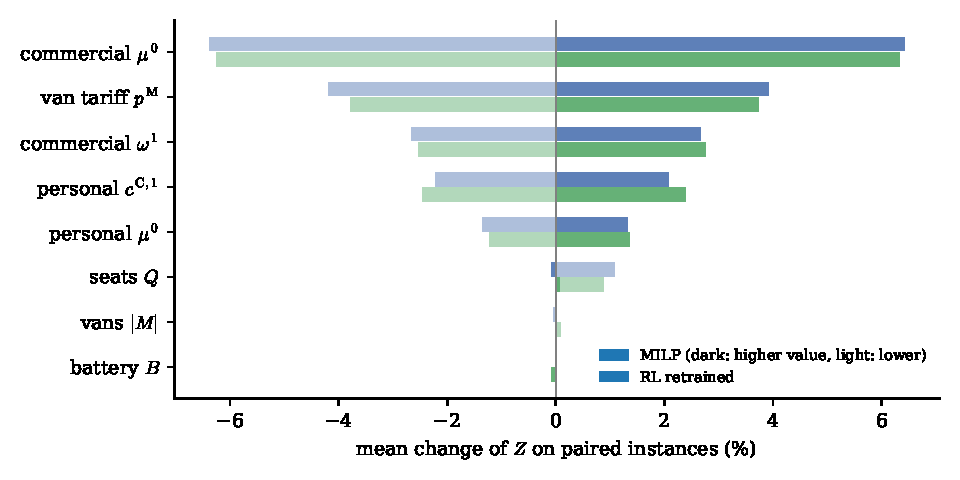
\includegraphics[width=0.8\textwidth]{figures/tornado.pdf}
\caption{Mean change of $Z$ for every variant, MILP and retrained RL.}\end{figure}
\begin{table}[H]\centering
\scriptsize
\caption{All factors sorted by their largest effect on $Z$ (mean $\Delta Z$ over paired instances). Elasticity: \% change of $Z$ per \% change of the factor (between the low and high variant; for the battery the high variant alone). Van-share changes in percentage points (MILP).}\label{tab:tornado}
\begin{adjustbox}{max width=\textwidth}\begin{tabular}{lrrrrrrrr}\toprule
factor & \shortstack{MILP\\low (\%)} & \shortstack{MILP\\high (\%)} & \shortstack{RL$_{\mathrm{rt}}$\\low (\%)} & \shortstack{RL$_{\mathrm{rt}}$\\high (\%)} & \shortstack{swing\\(points)} & \shortstack{elasticity\\of $Z$} & \shortstack{$\Delta$ van share\\personal, low} & \shortstack{$\Delta$ van share\\personal, high} \\ \midrule
commercial $\mu^{0}$ & $-$6.38 & +6.43 & $-$6.25 & +6.33 & 12.81 & +0.256 & $-$0.3 & $-$0.1 \\
van tariff $p^{\mathrm M}$ & $-$4.19 & +3.91 & $-$3.78 & +3.73 & 8.10 & +0.101 & +11.6 & $-$6.4 \\
commercial $\omega^{1}$ & $-$2.67 & +2.66 & $-$2.52 & +2.75 & 5.33 & +0.107 & $-$0.3 & $-$0.3 \\
personal $c^{\mathrm C,1}$ & $-$2.21 & +2.08 & $-$2.46 & +2.38 & 4.29 & +0.086 & $-$5.9 & +9.5 \\
personal $\mu^{0}$ & $-$1.35 & +1.33 & $-$1.22 & +1.36 & 2.68 & +0.054 & $-$0.1 & $-$1.0 \\
seats $Q$ & +1.08 & $-$0.08 & +0.88 & +0.07 & 1.16 & $-$0.017 & $-$8.3 & +1.7 \\
vans $|M|$ & $-$0.04 & +0.02 & +0.09 & +0.00 & 0.06 & +0.001 & $-$2.0 & +0.6 \\
battery $B$ & -- & $-$0.01 & -- & $-$0.07 & 0.01 & $-$0.000 & -- & $-$1.4 \\
\bottomrule\end{tabular}\end{adjustbox}\end{table}

\begin{itemize}
  \item \textbf{What moves $Z$}: \TopFactor{} (swing \TopSwing{} points), then the van tariff, the commercial downtime rate and the private owners' value of charging time. All four are customer parameters that are placeholders or only partly calibrated.
  \item \textbf{What moves decisions}: only the van tariff, the private owners' value of charging time and the seats per van change the van share by several points. The money sensitivities and the commercial downtime rate change $Z$ without changing who is served where.
  \item \textbf{What does not matter}: the number of vans (except for feasibility) and the battery.
\end{itemize}
\inshort{To make the results credible, measure the money sensitivity and downtime rate of commercial drivers and the private owners' value of station time; to steer who gets vans, use the tariff and the seats.}

\subsection{All ten experiments, measured with RL}\label{sec:allrl}
Only retrained RL was run on every experiment. Measured with it, the factors rank as follows ($^{\dagger}$: RL-only).
\begin{table}[H]\centering
\scriptsize
\caption{All eleven factors of the ten experiments, measured with retrained RL (the only method run on every experiment), sorted by their largest effect on $Z$. $^{\dagger}$: RL-only experiment, no MILP run. Elasticity: \% change of $Z$ per \% change of the factor between the low and high variant.}\label{tab:tornadorl}
\begin{adjustbox}{max width=\textwidth}\begin{tabular}{lcrrrrc}\toprule
factor & \shortstack{change of the\\factor, low / high (\%)} & \shortstack{RL$_{\mathrm{rt}}$\\low (\%)} & \shortstack{RL$_{\mathrm{rt}}$\\high (\%)} & \shortstack{swing\\(points)} & \shortstack{elasticity\\of $Z$} & \shortstack{MILP low / high\\(\%)} \\ \midrule
energy per EV$^{\dagger}$ & $-$25 / +25 & $-$21.82 & +22.19 & 44.01 & +0.880 & RL only \\
kW per gun$^{\dagger}$ & $-$50 / +100 & +20.13 & $-$12.30 & 32.42 & $-$0.216 & RL only \\
commercial $\mu^{0}$ & $-$25 / +25 & $-$6.25 & +6.33 & 12.58 & +0.252 & $-$6.38 / +6.43 \\
guns per station$^{\dagger}$ & $-$50 / +100 & +4.76 & $-$2.21 & 6.98 & $-$0.047 & RL only \\
van tariff $p^{\mathrm M}$ & $-$40 / +40 & $-$3.78 & +3.73 & 7.50 & +0.094 & $-$4.19 / +3.91 \\
commercial $\omega^{1}$ & $-$25 / +25 & $-$2.52 & +2.75 & 5.27 & +0.105 & $-$2.67 / +2.66 \\
personal $c^{\mathrm C,1}$ & $-$25 / +25 & $-$2.46 & +2.38 & 4.84 & +0.097 & $-$2.21 / +2.08 \\
personal $\mu^{0}$ & $-$25 / +25 & $-$1.22 & +1.36 & 2.58 & +0.052 & $-$1.35 / +1.33 \\
seats $Q$ & $-$33 / +33 & +0.88 & +0.07 & 0.81 & $-$0.012 & +1.08 / $-$0.08 \\
vans $|M|$ & $-$40 / +40 & +0.09 & +0.00 & 0.08 & $-$0.001 & $-$0.04 / +0.02 \\
battery $B$ & -- / +33 & -- & $-$0.07 & 0.07 & $-$0.002 & -- / $-$0.01 \\
\bottomrule\end{tabular}\end{adjustbox}\end{table}

\begin{figure}[H]\centering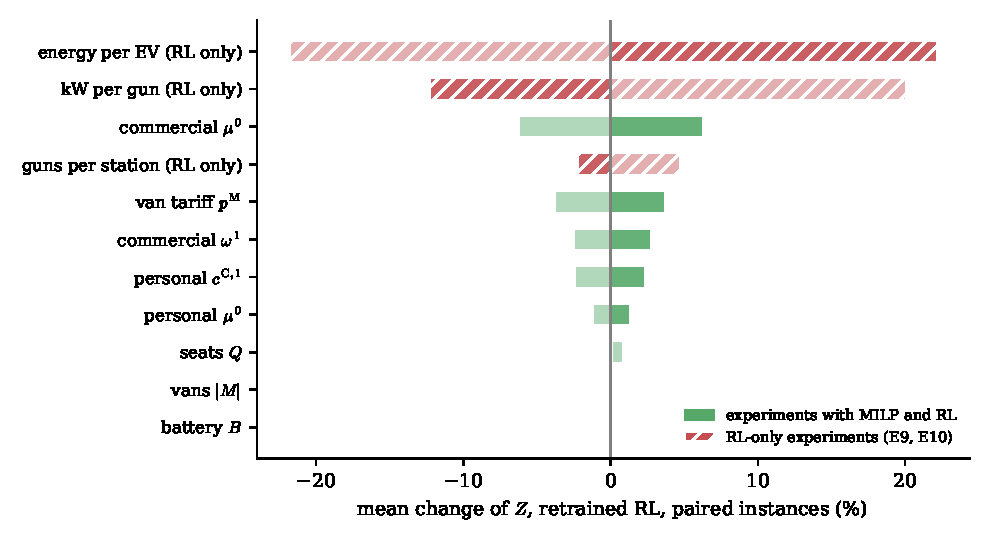
\includegraphics[width=0.78\textwidth]{figures/tornado_rl.pdf}
\caption{Mean change of $Z$ for every variant of the ten experiments, retrained RL (light: lower value, dark: higher value; hatched: RL-only experiments).}\end{figure}
\begin{itemize}
  \item The strongest factor of all is \TopFactorRl{} (swing \TopSwingRl{} points); station power ranks \RankPowerRl{} and guns per station \RankGunsRl{} of \NFactorsAll.
  \item The RL-only factors (E9, E10) cannot be checked against the MILP: their size rests on RL alone, whose effects on $Z$ were within about \EffDiffRtMean{} points of the MILP's on the other experiments.
\end{itemize}
\inshort{Energy per EV and station power move the cost far more than any customer parameter; the commercial money sensitivity comes next, ahead of the number of guns.}

\subsection{Utilisation across experiments}\label{sec:utilexp}
\begin{table}[H]\centering
\scriptsize
\caption{Utilisation of every variant against its own baseline on its paired instances (MILP and retrained RL; capacities $M$, $Q$, $B$ of the variant; arrows: baseline $\to$ variant).}\label{tab:utilexp}
\begin{adjustbox}{max width=\textwidth}\begin{tabular}{llrrcccccr}\toprule
variant & method & \shortstack{$\Delta$ gun time\\(pts)} & \shortstack{$\Delta$ van share\\of kWh (pts)} & \shortstack{fleet use\\(\% of $M$)} & \shortstack{seats\\(\% of $Q$)} & \shortstack{battery\\(\% of $B$)} & \shortstack{on the road\\(\% of $T$)} & \shortstack{van power\\used (\%)} & \shortstack{$\Delta$ installed\\capacity (pts)} \\ \midrule
personal $c^{\mathrm C,1}=7.5$ & MILP & +0.24 & $-$1.87 & 44$\to$43 & 79$\to$76 & 71$\to$68 & 68$\to$66 & 24.5$\to$23.1 & $-$0.00 \\
 & RL retrained & +0.12 & $-$1.11 & 44$\to$44 & 68$\to$65 & 62$\to$60 & 71$\to$69 & 24.7$\to$24.0 & $-$0.00 \\
personal $c^{\mathrm C,1}=12.5$ & MILP & $-$0.34 & +2.26 & 44$\to$47 & 79$\to$81 & 71$\to$74 & 68$\to$69 & 24.5$\to$25.0 & $-$0.00 \\
 & RL retrained & $-$0.23 & +1.23 & 44$\to$45 & 68$\to$71 & 62$\to$65 & 71$\to$72 & 24.8$\to$26.1 & +0.00 \\
commercial $\omega^{1}=4.5$ & MILP & +0.01 & $-$0.07 & 44$\to$43 & 79$\to$79 & 71$\to$71 & 68$\to$68 & 24.4$\to$24.5 & $-$0.00 \\
 & RL retrained & $-$0.06 & $-$0.03 & 44$\to$45 & 68$\to$67 & 62$\to$62 & 71$\to$71 & 24.7$\to$24.9 & +0.00 \\
commercial $\omega^{1}=7.5$ & MILP & +0.03 & $-$0.04 & 44$\to$44 & 79$\to$78 & 71$\to$70 & 68$\to$67 & 24.5$\to$24.0 & $-$0.00 \\
 & RL retrained & $-$0.03 & +0.04 & 44$\to$44 & 68$\to$68 & 62$\to$62 & 71$\to$71 & 24.7$\to$24.8 & $-$0.00 \\
personal $\mu^{0}=1.125$ & MILP & +0.01 & +0.00 & 44$\to$44 & 79$\to$79 & 71$\to$71 & 68$\to$69 & 24.5$\to$24.6 & $-$0.00 \\
 & RL retrained & $-$0.08 & +0.26 & 44$\to$44 & 68$\to$69 & 62$\to$63 & 71$\to$71 & 24.8$\to$25.5 & +0.00 \\
personal $\mu^{0}=1.875$ & MILP & +0.04 & $-$0.33 & 44$\to$44 & 79$\to$78 & 71$\to$71 & 68$\to$68 & 24.6$\to$24.4 & $-$0.00 \\
 & RL retrained & $-$0.04 & +0.04 & 44$\to$44 & 68$\to$68 & 62$\to$62 & 71$\to$71 & 24.7$\to$24.9 & +0.00 \\
commercial $\mu^{0}=1.125$ & MILP & +0.02 & $-$0.06 & 44$\to$44 & 79$\to$78 & 71$\to$71 & 68$\to$68 & 24.8$\to$24.6 & $-$0.00 \\
 & RL retrained & $-$0.01 & +0.03 & 44$\to$44 & 68$\to$68 & 62$\to$63 & 71$\to$71 & 24.8$\to$25.1 & +0.00 \\
commercial $\mu^{0}=1.875$ & MILP & +0.02 & $-$0.05 & 44$\to$44 & 79$\to$79 & 71$\to$71 & 68$\to$68 & 24.6$\to$24.4 & $-$0.00 \\
 & RL retrained & $-$0.06 & +0.08 & 44$\to$44 & 68$\to$68 & 62$\to$62 & 71$\to$71 & 24.7$\to$25.0 & +0.00 \\
$p^{\mathrm M}=15$ & MILP & $-$0.41 & +3.76 & 43$\to$48 & 79$\to$84 & 71$\to$77 & 68$\to$70 & 24.2$\to$24.9 & $-$0.00 \\
 & RL retrained & $-$0.24 & +1.45 & 44$\to$45 & 68$\to$71 & 62$\to$66 & 71$\to$72 & 24.7$\to$26.0 & +0.00 \\
$p^{\mathrm M}=35$ & MILP & +0.28 & $-$2.14 & 44$\to$42 & 79$\to$75 & 71$\to$67 & 68$\to$66 & 24.8$\to$23.3 & $-$0.00 \\
 & RL retrained & +0.22 & $-$1.72 & 44$\to$44 & 68$\to$63 & 62$\to$58 & 71$\to$66 & 24.7$\to$23.2 & $-$0.00 \\
3 vans & MILP & +0.09 & $-$0.36 & 40$\to$65 & 81$\to$82 & 73$\to$73 & 67$\to$68 & 22.3$\to$22.3 & +1.03 \\
 & RL retrained & +0.07 & $-$0.17 & 41$\to$67 & 69$\to$69 & 63$\to$63 & 69$\to$69 & 21.6$\to$21.1 & +1.17 \\
7 vans & MILP & $-$0.03 & +0.08 & 44$\to$32 & 79$\to$79 & 71$\to$71 & 68$\to$68 & 24.8$\to$24.7 & $-$1.01 \\
 & RL retrained & $-$0.07 & $-$0.02 & 44$\to$32 & 68$\to$67 & 62$\to$62 & 71$\to$71 & 24.8$\to$25.1 & $-$1.20 \\
4 seats per van & MILP & +0.20 & $-$1.33 & 43$\to$50 & 79$\to$91 & 71$\to$56 & 69$\to$62 & 24.8$\to$20.1 & $-$0.00 \\
 & RL retrained & $-$0.05 & +0.22 & 44$\to$51 & 67$\to$86 & 62$\to$53 & 71$\to$65 & 24.8$\to$21.5 & +0.00 \\
8 seats per van & MILP & $-$0.01 & +0.20 & 44$\to$43 & 79$\to$62 & 71$\to$74 & 68$\to$69 & 24.4$\to$24.9 & +0.00 \\
 & RL retrained & $-$0.07 & +0.03 & 44$\to$43 & 68$\to$52 & 62$\to$64 & 71$\to$71 & 24.7$\to$25.7 & $-$0.00 \\
battery 200 kWh & MILP & +0.05 & $-$0.13 & 44$\to$43 & 79$\to$79 & 71$\to$54 & 68$\to$68 & 24.6$\to$24.8 & $-$0.00 \\
 & RL retrained & $-$0.07 & +0.29 & 44$\to$44 & 68$\to$69 & 62$\to$48 & 71$\to$71 & 24.7$\to$25.5 & +0.00 \\
\bottomrule\end{tabular}\end{adjustbox}\end{table}

\begin{figure}[H]\centering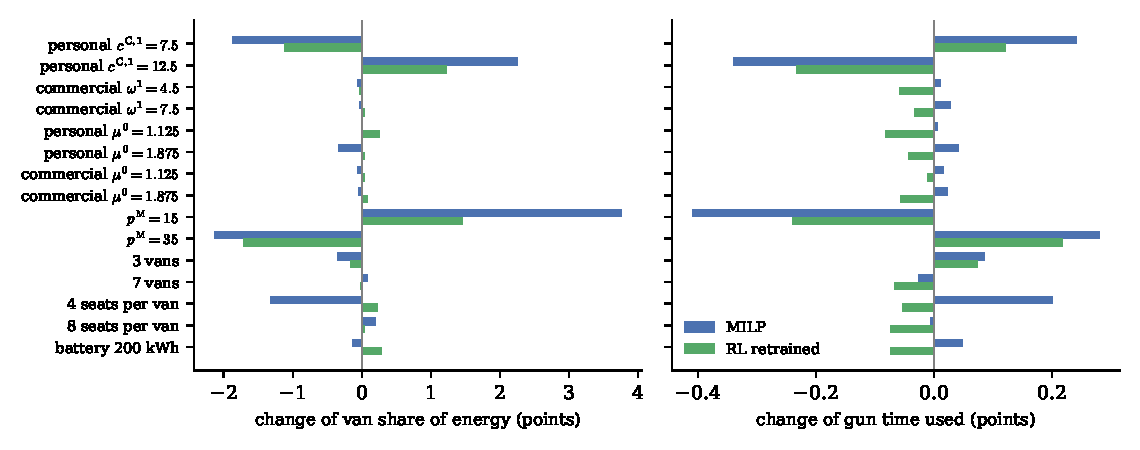
\includegraphics[width=0.98\textwidth]{figures/util_experiments.pdf}
\caption{Change of the van share of energy and of the gun time used for every variant, MILP and retrained RL.}\end{figure}
\begin{itemize}
  \item \textbf{E2 vans: the extra capacity is not used.} With 7 vans the fleet use falls from \UXBEtwoVansHiFleetMilp\pct{} to \UXEtwoVansHiFleetMilp\pct{}: the same number of vans leave (\UXBEtwoVansHiVansUsedMilp{} $\to$ \UXEtwoVansHiVansUsedMilp) and the van share of energy changes by \UXKwhEtwoVansHi{} points. With 3 vans the fleet use rises to \UXEtwoVansLoFleetMilp\pct; on the instances that stay feasible nothing else changes.
  \item \textbf{E2 seats: extra seats stay empty, fewer seats are filled.} With 8 seats the seat use falls from \UXBEtwoSeatsHiSeatMilp\pct{} to \UXEtwoSeatsHiSeatMilp\pct{} and the battery use rises (\UXBEtwoSeatsHiBatteryMilp\pct{} $\to$ \UXEtwoSeatsHiBatteryMilp\pct); with 4 seats the seats are \UXEtwoSeatsLoSeatMilp\pct{} used and the van share of energy changes by \UXKwhEtwoSeatsLo{} points.
  \item \textbf{E8: with 200\,kWh} the battery use falls from \UXBEeightBatHiBatteryMilp\pct{} to \UXEeightBatHiBatteryMilp\pct{} of $B$, and \UXEeightBatHiBninetyMilp\pct{} of vans draw more than 90\pct; nothing else moves.
  \item \textbf{E1 shifts energy between stations and vans}: $p^{\mathrm M}=15$ moves \UXKwhEonePMLo{} points of the energy to vans (fleet use \UXBEonePMLoFleetMilp\pct{} $\to$ \UXEonePMLoFleetMilp\pct, seats \UXBEonePMLoSeatMilp\pct{} $\to$ \UXEonePMLoSeatMilp\pct), $p^{\mathrm M}=35$ \UXKwhEonePMHi{} points.
  \item \textbf{E5 personal} moves energy the same way (\UXDEfivePersHiVanEnergyMilp{} points at $c^{\mathrm C,1}=12.5$); \textbf{E5 commercial and E6} move it by less than half a point.
  \item The installed-capacity utilisation changes only when the fleet changes ($M=3$: \UXDEtwoVansLoSystemMilp{} points); the guns' time used changes by less than half a point in every variant.
  \item RL moves utilisation in the same direction as the MILP where the MILP effect is large (E1, E5 personal), with a smaller amplitude for the van share of energy; with 4 seats it does not shift energy from vans to stations as the MILP does.
\end{itemize}
\inshort{None of the variants makes the infrastructure scarce: more vans or seats stay idle, a bigger battery stays partly empty; only the van tariff and the private value of charging time move a few points of energy between stations and vans.}

\subsection{Can RL replace the MILP for experiments?}\label{sec:rlexp}
\begin{figure}[H]\centering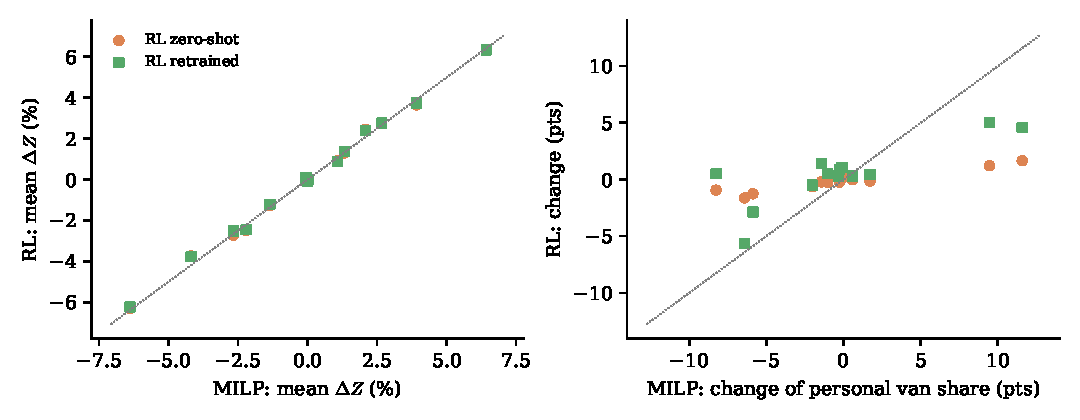
\includegraphics[width=0.92\textwidth]{figures/effects_methods.pdf}
\caption{Effect of every variant measured by RL against the MILP: change of $Z$ (left) and of the private van share (right).}\end{figure}
\begin{table}[H]\centering
\small
\caption{The 15 retrained RL models and the gap of both RL runs to the MILP of the same variant.}\label{tab:retrain}
\begin{adjustbox}{max width=\textwidth}\begin{tabular}{lrrrrr}\toprule
model trained on & minutes (GPU) & best epoch & \shortstack{validation cost\\RL / greedy} & \shortstack{gap to MILP\\zero-shot (\%)} & \shortstack{gap to MILP\\retrained (\%)} \\ \midrule
personal $c^{\mathrm C,1}=7.5$ & 38 & 201 & 0.970 & 0.56 & 0.56 \\
personal $c^{\mathrm C,1}=12.5$ & 39 & 200 & 0.969 & 1.22 & 1.14 \\
commercial $\omega^{1}=4.5$ & 40 & 145 & 0.971 & 0.82 & 0.98 \\
commercial $\omega^{1}=7.5$ & 39 & 148 & 0.967 & 0.83 & 0.86 \\
personal $\mu^{0}=1.125$ & 39 & 188 & 0.969 & 0.92 & 0.95 \\
personal $\mu^{0}=1.875$ & 40 & 180 & 0.969 & 0.80 & 0.84 \\
commercial $\mu^{0}=1.125$ & 39 & 183 & 0.968 & 0.87 & 0.91 \\
commercial $\mu^{0}=1.875$ & 38 & 200 & 0.971 & 0.80 & 0.79 \\
$p^{\mathrm M}=15$ & 39 & 186 & 0.967 & 1.31 & 1.25 \\
$p^{\mathrm M}=35$ & 40 & 148 & 0.972 & 0.58 & 0.63 \\
3 vans & 38 & 186 & 0.958 & 0.91 & 0.96 \\
7 vans & 38 & 181 & 0.965 & 0.84 & 0.81 \\
4 seats per van & 40 & 188 & 0.971 & 0.69 & 0.65 \\
8 seats per van & 38 & 162 & 0.970 & 0.86 & 0.98 \\
battery 200 kWh & 39 & 197 & 0.969 & 0.84 & 0.77 \\
baseline model & 39 & 180 & 0.969 &  &  \\
\bottomrule\end{tabular}\end{adjustbox}\end{table}

\begin{itemize}
  \item \textbf{Effects on $Z$}: the mean effect of a variant differs from the MILP's by \EffDiffRtMean{} points on average (at most \EffDiffRtMax) for retrained RL and \EffDiffZsMean{} (at most \EffDiffZsMax) zero-shot; the sign agrees in \SignAgreeRt{} (retrained) and \SignAgreeZs{} (zero-shot) of \NVariants{} variants, the exceptions being variants whose MILP effect is about zero.
  \item \textbf{Effects on decisions}: of the \VanEffBig{} variants that move the MILP's private van share by more than half a point, RL moves it the same way in \VanEffSignAgree{}, with about \VanEffRatio{} of the amplitude.
  \item \textbf{Retraining} (\RetrainMinMean{} minutes per variant, \RetrainMinTotal{} GPU-hours in total) does not lower the gap to the MILP on average (\GapZsAll\pct{} zero-shot, \GapRtAll\pct{} retrained; better in \RtBetterCount{} of \NVariants), but it makes the van shares respond more strongly (E1).
\end{itemize}
\inshort{RL, even zero-shot, measures how $Z$ reacts to an assumption almost as the MILP does; for how decisions react it gets the direction right but about half the size.}

%=====================================================================
\section{Robustness and caveats}
\begin{itemize}
  \item \textbf{Time-limit plans.} Effects below about 0.1 points are within the noise of unfinished MILP runs; the direction check settles their sign only on optimal pairs.
  \item \textbf{Congestion only in unfinished instances.} All queues and commercial van use at peak are in time-limit plans; peak results rest on two independent methods, not on proofs.
  \item \textbf{Peak label.} The median label of formulation 4 counts the start-of-period burst as off-peak; the pooled pressure terciles should be used (and \code{share\_van\_peak\_\%} in \code{runs.csv} read with care).
  \item \textbf{One factor at a time}; interactions (cheaper vans and more seats) are not tested.
  \item \textbf{One RL training per model} and one seed; the RL numbers carry the spread of training.
  \item \textbf{E9 and E10 are RL only}: no MILP run (no gap, no direction check) and no zero-shot run; RL's validity losses there may include instances that are feasible but that RL fails to solve.
  \item \textbf{Placeholders}: apart from the segment share and incomes, the customer parameters are reasoned values; the experiments show how much each matters, not its true value.
\end{itemize}

%=====================================================================
\section{Summary of findings and recommendations}
\begin{enumerate}
  \item The job is sound: \DirBad{} direction violations in \DirPairs{} optimal pairs; RL and MILP agree on feasibility except where only RL finds a plan.
  \item RL is \GapMean\pct{} dearer and \SpeedUp{} times faster; it takes the same decision for \AgreeFree\pct{} of free-choice EVs but gives too few vans to rich private owners.
  \item At peak, queues push poor commercial drivers to vans and take seats from private owners; RL reproduces the commercial part. The effect lives only in instances the MILP does not finish, and $\pm25\pct$ of the downtime rate does not change it.
  \item $Z$ depends most on the commercial money sensitivity $\mu^0$, then on the van tariff, the commercial downtime rate and the private value of charging time: measure these first.
  \item The van tariff and the private value of charging time decide who gets vans; a tariff equal to the station's helps rich private owners most and costs the operator more.
  \item More vans make short-horizon instances feasible; more seats lower the cost up to 6; the battery does not matter, so van recharging can be left out.
  \item For screening assumptions RL is good enough (effects on $Z$ within about \EffDiffRtMean{} points); for who gets vans, use the MILP.
  \item Among physical inputs (RL only), energy per EV and station power dominate: $\pm$25\pct{} energy moves $Z$ by \dZEtenDemLoRt\pct{} / \dZEtenDemHiRt\pct, half the station power by \dZEninePowLoRt\pct; cutting station capacity or adding energy loses short-horizon instances.
  \item The infrastructure is far from its limits (a gun busy \UGunMilp\pct{} of the period, installed capacity \USystemMilp\pct{} used, vans waiting \UIdleVanMilp\pct{} of their road time); only the van seats are nearly full, and no variant of E1--E8 makes guns, vans or batteries scarce; only cutting station capacity (E9) does.
\end{enumerate}

\vspace{6pt}
{\footnotesize Generated from \code{2026-11-22\_formulation\_4/*/results/*/runs.csv}, \code{plan.csv}, the RL \code{train\_meta.json} files and the formulation-4 data by \code{make\_results\_report.py}, \code{peak\_analysis.py}, \code{infra\_analysis.py} and \code{rl\_only\_analysis.py} in this folder, with the shared definitions of \code{../common/infra.py}.}

\end{document}
